\clearpage
\newpage
\subsection{Comparing AI Feedback Against Alternative Measures of Diversity}\label{main:alt_feedback}

\begin{table}[t]
\caption{\textbf{QDAIF outperforms QD with embedding feedback (QDEF) according to human evaluation in human QD score and quality, when the difference is in feedback type for each base method.}. The mean of Human QD score and quality are computed for the set of each method/run. The differences between the two evaluators for QD score and Quality are shown. Agreement between human and AI feedback on diversity labels given is slightly higher across QDAIF results compared to QDEF results, as well as on agreement between two annotators.}
\label{table:ef_vs_aif}
\centering
\scriptsize
\begin{tabular}{@{}lcccccc@{}}
\toprule
\textbf{Method} &
\makecell[c]{\textbf{Human}\\\textbf{QD score}} & 
\makecell[c]{\textbf{QD score}\\\textbf{range}} &
\makecell[c]{\textbf{Quality}\\\textbf{rating}} &
\makecell[c]{\textbf{Quality}\\\textbf{range}}  & 
\makecell[c]{\textbf{Human-AI}\\\textbf{agreement}} & 
\makecell[c]{\textbf{Human}\\\textbf{agreement}}  \\
\midrule
        QDEF, LMX, Zero-Shot Init  & 0.242 & 0.050 & 1.300 & 0.600 & 0.500 & 0.400  \\ 
        QDEF, LMX, Seeded Init  & 0.308 & 0.050 & 1.700 & 0.600 & 0.600 & 0.600  \\ 
        QDEF, LMX-Replace, Zero-Shot Init  & 0.417 & 0.233 & 2.100 & 1.000 & 0.800 & 0.600  \\ 
        QDEF, LMX-Replace, Seeded Init  & 0.500 & 0.200 & 2.300 & 1.000 & 0.800 & 1.000  \\ 
        QDAIF, LMX, Zero-Shot Init  & 0.350 & 0.300 & 1.700 & 1.400 & 0.800 & 1.000  \\ 
        QDAIF, LMX, Seeded Init  & 0.617 & 0.167 & 3.200 & 1.200 & 1.000 & 1.000  \\ 
        QDAIF, LMX-Replace, Zero-Shot Init  & 0.833 & 0.267 & 4.300 & 1.000 & 0.600 & 0.600  \\ 
        QDAIF, LMX-Replace, Seeded Init & 0.739 & 0.078 & 3.700 & 0.600 & 0.700 & 0.800 \\ 
\bottomrule
\end{tabular}
\end{table}

To understand the effect of fuzzy evaluation tools as a component of our QD setup, we tested the use of an alternative method of feedback compared to our default method (AI feedback) in the MAP-Elites pipeline: semantic embedding feedback \citep{reimers2019sentence}. For this method, we used a 13B embedding model\footnote[1]{\url{https://aleph-alpha.com/luminous\%2Dexplore\%2Da\%2Dmodel\%2Dfor\%2Dworld\%2Dclass\%2Dsemantic\%2Drepresentation/}}, based on the architecture described in \citet{sgpt}, with an asymmetric search setup to measure the distance between a generated text (document embedding) and a query embedding for a desired measure (e.g. "This is a positive opinion"). To compute a diversity measure that can be defined on an axis, we first get the cosine distances between the document embedding and each of two opposing attribute query embeddings. From this, we can measure how close the document embedding is to one attribute compared to the other, and obtain a single diversity measure normalized in the range [0, 1]. We use the same method for quality feedback, with a query that aims to measure the relevance of generated texts to a specific domain. The cosine similarity is used here as a quality score, with negative values being clipped to 0. Additional setup details are shown in \cref{app:ef_setup_lmx}. Since the subjective quality of the resulting elites (of creative texts) is more informative of the method's potential in further applications for practical synthetic data generation, We conducted a human study in addition to the reporting of QD score stats as part of our results.

We display performance statistics from our runs (QD Score) as well as human evaluation scores on elite samples in \cref{table:ef_vs_aif}. We observe from our human study that using AI feedback as the evaluator instead of semantic embedding feedback for every variation of the QD run setup potentially leads to subjectively better generations. This is likely due to more prominent reward hacking \citep{skalse2022defining,lehman2019surprising} occurring in runs using embedding feedback, where the highest quality score texts end up being very similar to the query "An opinion piece about eating vegetables and plant-based foods", while not optimizing for the subjective quality of texts in different bins. Qualitative analysis of human-evaluated sets of texts from QD with embedding feedback is shown in \crefrange{app:table_eval_opinions_ef_near_seeded}{app:table_eval_opinions_ef_replace_zero}. Furthermore, agreement between human and AI feedback on text diversity labels was slightly higher across QDAIF sets compared to QD with embedding feedback (QDEF) sets. Overall, AI feedback outperforms the alternative measure of semantic embedding feedback, by guiding the generation of texts that are more preferred by humans, and by serving as a better evaluator for quality and diversity measures than embedding feedback.

\clearpage
\newpage
\subsection{On Scaling LMs for Mutation}\label{app:scaling_discussion}
Previous work has consistently shown that LMs demonstrate improved capabilities in various task-based benchmarks at larger scales \citep{kaplan2020scaling,chowdhery2022palm,chung2022scaling}. This applies to performance in solving tasks through in-context learning, which LMX is based on. Prior work in LMX \citep{meyerson2023language} has found that a relationship between model scaling and performance of mutations can be observed when evolving binary strings in a search domain. Interestingly, experiments in LMX as well as ELM \citep{lehman2022evolution} observed that in some cases, emerging capabilities in mutation ability appear for reasonably small LMs, but may not scale with a clear trend.

Firstly, we show the QD score performance between runs in \cref{app:fig_scaling}. The standard error in the score across 5 seeds is also shown. We observed that the QD score from the 70B runs converged to a lower point compared to the 13B and 30B runs, which have comparable scores. This highlights a trend between model size and QD score that is not directly proportional. Although suggestive trends are not seen here, a study based on subjective feedback is still necessary for a deeper understanding of the performance of each experiment.

We observed from the human feedback evaluation a trend in the quality ratings, with average quality scores from each experiment set of: 3.43 (13B), 3.60 (30B), and 4.03 (70B). The quality score increases with an increase in model size used, with a higher jump in score for generated stories from the 70B runs.

In terms of the agreement on the genres of evaluated stories between AI feedback and human feedback, we observed the following percentage rates in the following sets: 80.0\% (13B), 73.3\% (30B), and 73.3\% (70B). There is a slight decrease in agreement for texts from the 30B and 70B runs. We found that evaluators differed more frequently in their labels on stories deemed as "neutral" or "romance" according to AI feedback, suggesting that the use of the prompt pool in combination with larger models might lead to generated texts with misaligned AI evaluations on the genre. Still, these agreement rates indicate a good alignment between AI and human feedback.

\begin{figure}[!t]
    \centering
    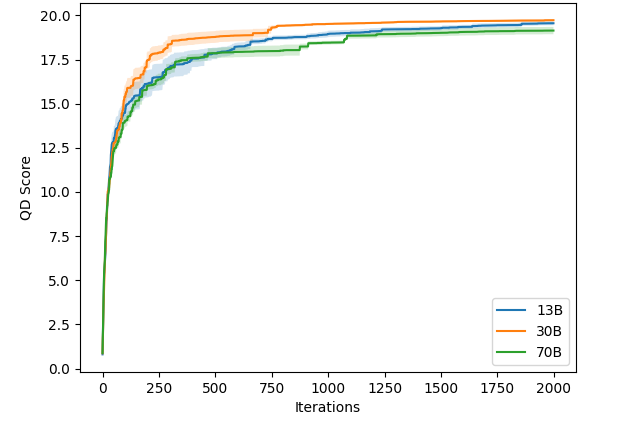
\includegraphics[height=0.5\textwidth]{main_figures/extensions/model_size.png}
    \caption{\textbf{QD score plots for different LMX model sizes on the Stories - Genre domain}. There is no clear trend in scaling model size with QD score.}
    \label{app:fig_scaling}
\end{figure}

\clearpage
\newpage
\subsection{On Few-Shot AI Feedback Prompting}\label{app:few_shot_aif_discussion}
Instruction-following LMs are typically trained to align the model towards generating better answers to zero-shot prompts \citep{wei2021finetuned,ouyang2022training}. However, few-shot prompting with exemplars was shown to be effective in some aspects with instruction-tuned LMs, especially towards understanding task structure and improving robustness to prompting variations \citep{wei2021finetuned}.

In terms of the average human-evaluated quality, we see a drop in subjective quality for the set of stories from 2-shot AI feedback runs (3.10) in comparison to zero-shot AI feedback runs (3.43). We observed for the other sets that this score increases for the 4-shot set (3.93) and the 8-shot set (4.03). Furthermore, we see that this trend is mostly consistent when we consider the scores for each bin category. This suggests an improvement in QDAIF's ability to discover texts that are perceived to be of higher quality according to human feedback when we use a higher number of in-context examples during AI feedback evaluation.

In terms of the agreement between AI feedback and human feedback, we see a drop in average agreement for ratings that were given to stories in the few-shot feedback experiment sets, with 50.0\% (2-shot), 66.7\% (4-shot), and 56.7\% (8-shot) agreement on sets, compared to 80.0\% for zero-shot (default). The level of disagreement occurs more frequently on stories evaluated to have the romance genre. Additionally, evaluators labeled samples from the few-shot sets as "horror" or "neutral" more frequently than "romance", while the proportion of labels given to samples from the zero-shot set was more uniform.

The performance may vary due to the ordering of in-context examples in our few-shot prompts (in \cref{app:few_shot_feedback_details}, as shown in \citet{lu2021fantastically}. Furthermore, the nature and wording of input-output exemplars/tasks could also influence the performance, in addition to some variation due to the nature of subjective evaluation.

\subsection{On the Initialization Method for QDAIF}\label{app:init_method_discussion}
\begin{figure}[!t]
    \centering
    \hspace*{-1.5cm}
    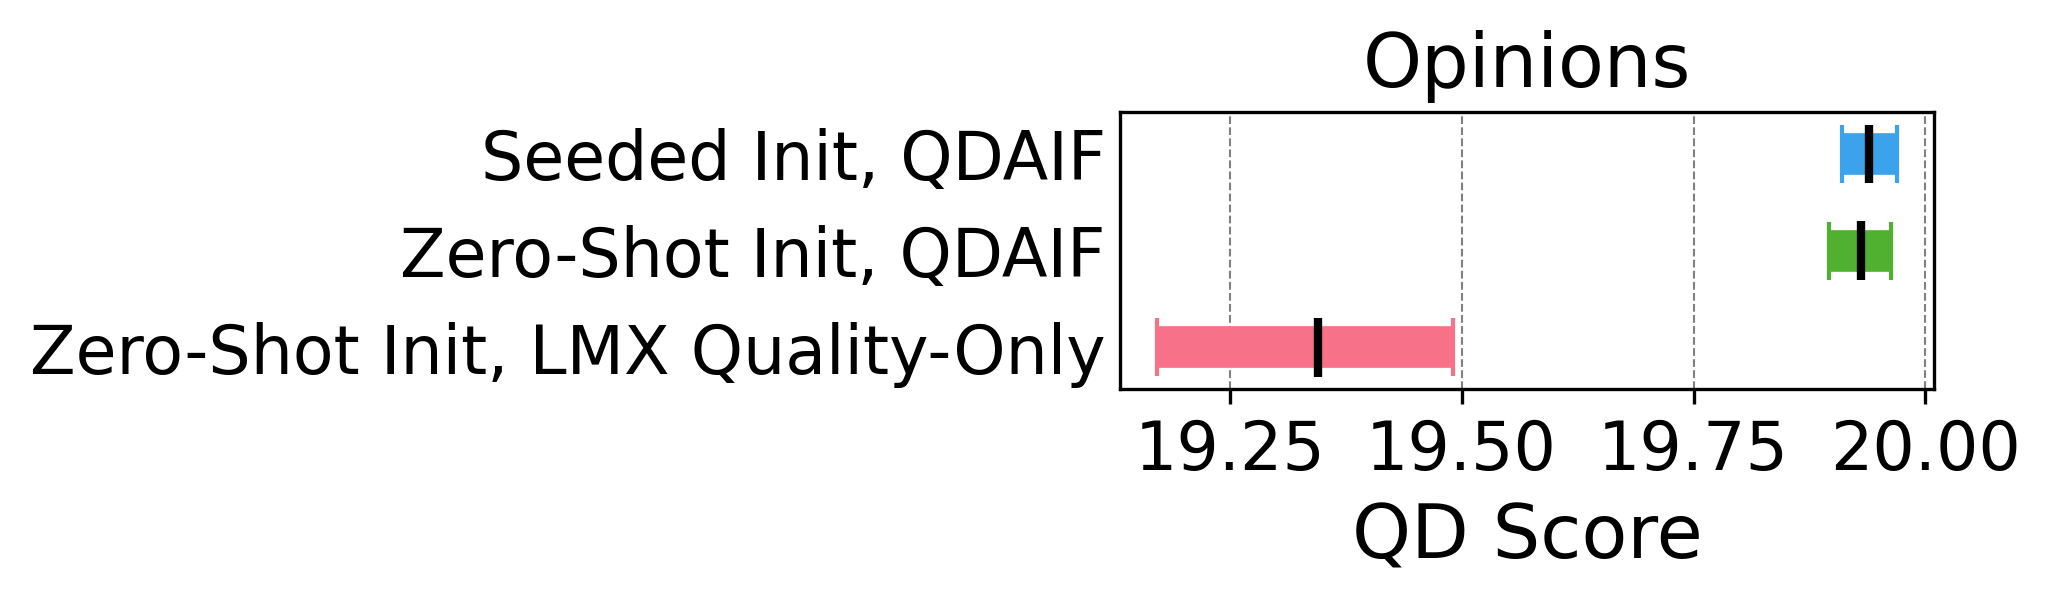
\includegraphics[height=0.08\textheight]{main_figures/perf_bars/seed_vs_zero_opinions.png}
    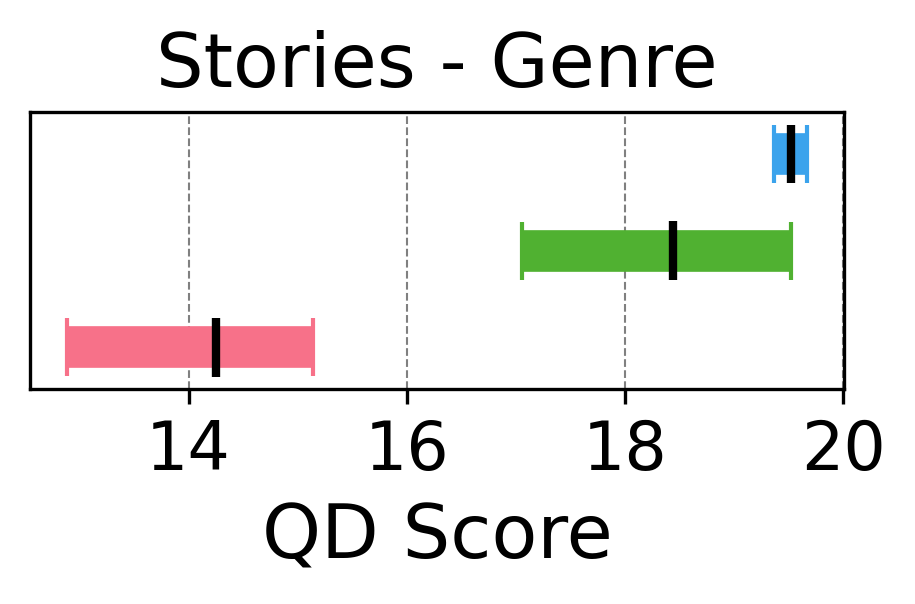
\includegraphics[height=0.08\textheight]{main_figures/perf_bars/seed_vs_zero_stories_genre.png}
    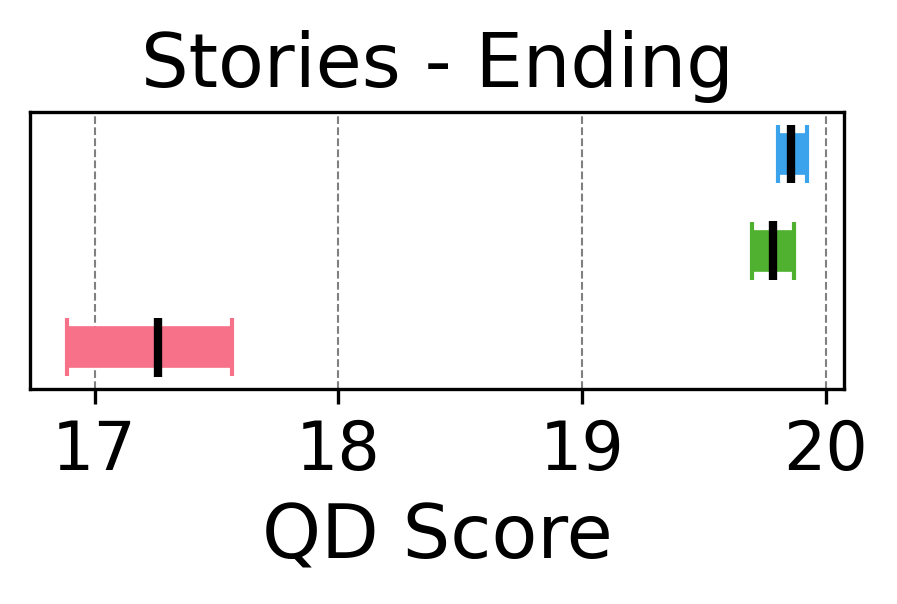
\includegraphics[height=0.08\textheight]{main_figures/perf_bars/seed_vs_zero_stories_ending.png}
    \vspace{-0.45cm}
    \caption{\textbf{QD score Performance between Seeded Init and Zero-Shot}. Performance stats with mean, interquartile mean (IQM) and bootstrapped 95\% CI, across 5 random seed runs. Seeded Init is potentially better, but within the CI of Zero-Shot Init. In the Stories - Genre domain, the CI of Zero-Shot Init runs is much wider, indicating significant variation in performance for different random seeds.}
    \label{fig:seed_vs_zero_init_perf}
\end{figure}

Recent results from LMX demonstrated successful optimization when the search was initialized by evolving a set of pre-existing seed examples (e.g. examples of equations, quotes, text-to-image prompts, code) \citep{meyerson2023language}. At the same time, previous applications of QD methods demonstrated successful search outcomes when using random initialization in different domains, such as in robotics, and latent space illumination of generative models \citep{cully2015robots, fontaine2021differentiable,bhatt2022deep}.

We compared the performance between QDAIF with \qdaifinitseed{} against \qdaifinitzero{} and a baseline method \basefour{} initialized with \qdaifinitzero. From \cref{fig:seed_vs_zero_init_perf}, we can see that there is potential improvement in QD score when using \qdaifinitseed{} compared to \qdaifinitzero, but the difference may not be significant. However, the difference is clear on the lower performance of \basefour{} with \qdaifinitzero. This suggests that \qdaifinitzero{} is viable for QDAIF. Still, we need to analyze the effect of the initialization on qualitative samples of elite texts. We also compared the effects of initialization on subjective quality-diversity of texts (see \cref{table:mean_human_eval_qdaif}). Sets of texts discovered by \qdaifinitseed{} within single runs were found to be subjectively higher-quality and more diverse compared to sets from \qdaifinitzero{} (0.772 vs. 0.383 subjective QD score). This suggests potential reward hacking (described for RL problems in \citet{skalse2022defining,lehman2019surprising} during the search with \qdaifinitzero{} runs, where potentially out-of-distribution texts can evolve to optimize the AI feedback quality score of solutions, but lead to subjectively low-quality texts across bins.

\subsection{On the Mechanisms of Mutation for QDAIF}\label{app:mutation_method_discussion}
\begin{table}[!t]
\caption{Mean stats, human eval scores, QDAIF methods. LMX-Replace outperforms LMX when using Zero-Shot Init.}
\vspace{0.4cm}
\label{table:mean_human_eval_qdaif}
\centering
\small
\begin{tabular}{lcccc}
\toprule
\textbf{Method} &
\textbf{QD score} & \textbf{Quality} & \textbf{H-AI agreement} & \textbf{H agreement }  \\
\midrule
LMX w/ Zero-Shot Init & 0.383 & 2.233 & 0.600 & 0.600  \\
LMX-Replace w/ Zero-Shot Init & 0.540 & 2.800 & 0.700 & 0.800  \\
\midrule
LMX w/ Seeded Init & 0.772 & 3.900 & 0.833 & 0.800  \\
LMX-Replace w/ Seeded Init & 0.763 & 3.800 & 0.800 & 0.800 \\
\bottomrule
\end{tabular}
\end{table}


Prior work on ELM highlights the versatility of LMs in applying a variety of potential mutation methods, such as in the form of git diffs, or prompting to directly evolve text/code \cite{lehman2022evolution}. However, studying the potential effects of different LM-based mutation operators on population-level evolvability (focused on future creative potential \cite{lehman2016critical}) remains a challenge. Towards understanding the potential of different mutation methods in terms of population-level evolvability of niches, we compare LMX(-Near) (default) (as tested in \cite{meyerson2023language}) against LMX-Replace in terms of resulting generated texts across different runs.

To observe the impact of different mutation methods on the dynamics of the population during search (along with the impact on performance), we implemented and tested an additional method called LMX-Replace. This method evolves few-shot prompts using a larger pool of prompt candidates than that of LMX(-Near) and carries out a slower mutation process by modifying only one few-shot prompt example (instead of all examples) during search iterations. We give a detailed comparison between the methods in \cref{app:lmx_method}.

We observed an improvement to the resulting generated text sets from runs using LMX-Replace in comparison to LMX for the \qdaifinitzero{} case, according to human evaluation results highlighted in \cref{table:mean_human_eval_qdaif}. We see that the subjective QD score and the quality rating from human evaluators were higher on average across the tested domains (and improvements within domain-by-domain comparisons also, highlighted in \cref{app:table_human_eval_baselines_vs_aif}). Given that it may not be desirable to constrain the search with \qdaifnearseed, LMX-Replace can act as an alternative mutation method to steer the dynamics of population search towards subjectively improved outputs.

The introduction of an archive depth was used for the creation and maintenance of a prompt pool for LMX-Replace (cf. \cref{app:qdaif_lmx}). Future works could explore the usage of depth in MAP-Elites archives for domains where uncertainty (or subjectivity) influences the evaluation of solutions, as was previously studied in \citet{flageat2020fast,flageat2023uncertain}.

\clearpage
\newpage
\subsection{On Coverage and Best Quality Solutions across Domains}\label{app:coverage_best_solution_discussion}
\cref{app:fig:qd_vs_non_qd_coverage} shows performance plots measuring the coverage of the archive (i.e. how many bins in the search space are filled with at least one solution). \cref{app:fig:qd_vs_non_qd_max_fitness} shows performance plots measuring the quality score of the best solution found across the whole search (existing in one of the defined bins).

QDAIF often discovers the best overall solutions during search that have higher quality scores than the best overall solutions found from other methods. This is likely enabled by the goal-switching mechanism of QD approaches \citep{mouret2015illuminating,gaier2019quality}. Overall, QDAIF can jointly optimize the quality and diversity of solutions, outperforming other methods in most comparisons, and highlighting contributions to successful gains in QD score.

\begin{figure}[ht]
    \centering
    \hspace*{-0.8cm}
    
\includegraphics[height=0.08\textheight]{main_figures/perf_bars/qd_vs_non_qd_opinions_cov.png}
    
\includegraphics[height=0.08\textheight]{main_figures/perf_bars/qd_vs_non_qd_story_genre_cov.png}
    
\includegraphics[height=0.08\textheight]{main_figures/perf_bars/qd_vs_non_qd_story_ending_cov.png}
    
\includegraphics[height=0.08\textheight]{main_figures/perf_bars/qd_vs_non_qd_story_genre_ending_cov.png}
    \vspace{-0.45cm}
    \caption{\textbf{QDAIF significantly outperforms baselines in the percentage of available bins covered by solutions in all domains}. Coverage stats with mean bootstrapped 95\% CI, across 5 random seed runs. The maximum possible coverage is 1. In some cases, methods achieve maximum coverage across all runs. The advantage of QD approaches is shown in their ability to discover more solutions that cover a wider search space, in addition to finding high-quality solutions (cf. \cref{app:fig:qd_vs_non_qd_max_fitness}).}
    \label{app:fig:qd_vs_non_qd_coverage}
\end{figure}

\begin{figure}[ht]
    \centering
    \hspace*{-0.8cm}
    
\includegraphics[height=0.08\textheight]{main_figures/perf_bars/qd_vs_non_qd_opinions_max.png}
    
\includegraphics[height=0.08\textheight]{main_figures/perf_bars/qd_vs_non_qd_story_genre_max.png}
    
\includegraphics[height=0.08\textheight]{main_figures/perf_bars/qd_vs_non_qd_story_ending_max.png}
    
\includegraphics[height=0.08\textheight]{main_figures/perf_bars/qd_vs_non_qd_story_genre_ending_max.png}
    \vspace{-0.45cm}
    \caption{\textbf{QDAIF and \basefour{} both optimize for the quality of the best solution found overall}. Best solution quality stats with mean bootstrapped 95\% CI, across 5 random seed runs. The maximum possible quality score is 1. QDAIF is more often able to achieve a higher score than \basefour{} in \textbf{Opinions} and \textbf{Stories - Ending}, while also outperforming in terms of coverage (cf. \cref{app:fig:qd_vs_non_qd_coverage}). In the 2D Stories - Genre and Ending domain, \basefour{} finds a solution with higher best quality more often than QDAIF, while still lagging in coverage. It is likely that QDAIF can find the best solutions with higher maximum quality more often in some domains because of the maintenance of diverse elite solutions that enable more possibilities to maximize the objective function, especially when the search begins to focus on refining existing solutions instead of covering unfilled bins \citep{gaier2019quality}. To save on compute, we reuse the generated (iterations of) texts from the baselines to compute independent stats comparisons as they do not use diversity measures during a search, unlike QDAIF which depends also on the defined diversity axes to conduct a successful search. We can compute independent QD score stats for baselines using the same 5 reruns, but in the \textbf{Stories} domains, the best solution quality remains the same.}
    \label{app:fig:qd_vs_non_qd_max_fitness}
\end{figure}

\clearpage
\newpage
\subsection{On Comparisons between QDAIF and Diversity-Seeking Baselines}\label{app:diversity_baselines}
We compared QDAIF against explicit diversity-seeking baseline methods. One baseline, \basefive, is based on n-gram-based filtering with ROUGE-L similarity \citep{lin2004rouge}, as done in Self-Instruct \citet{wang2022self}. They followed a similar approach of maintaining a few-shot prompt pool to generate diverse solutions (with diversity maintained by adding generated texts to a prompt pool if different enough to other existing solutions based on n-gram matching), in their case, for the generation of diverse instruction prompts towards the creation of a diverse, high-quality synthetic instruction tuning dataset. Another baseline is based on Novelty Search (NS) \citep{lehman2011abandoning}, a diversity-seeking algorithm that was proven to be more sample efficient than single-objective approaches (the diversity-only equivalent of \basefour, which only optimizes for solution quality) in discovering desired solutions to problems with many local optima, and also studied in prior works introducing the QD illumination problem (i.e. improving QD score \citep{pugh2016quality}). Unlike \basefive, NS aims to encourage diversity within an arbitrarily defined space of diversity. To make NS comparable with QDAIF, we introduce Novelty Search through AI Feedback (NSAIF) as the method that seeks diversity in domains where diversity is defined by AI feedback axes. We denote this baseline as \basesix. As with all methods, these baselines are initialized with the prompt pool specified in \cref{app:seed_pools}. We describe the baseline implementations in more detail in \cref{app:diversity_baselines_setup}, including variants of these baselines with quality AI feedback (QAIF) filters as a minimum criterion for diversity search \citep{lehman2010revising}.

\textbf{Results.} \cref{app:fig:extended_baselines_qd_score} shows QD score performance plots comparing QDAIF against diversity-seeking baselines, baselines that also aim for quality and diversity in solutions, and other baselines. QDAIF consistently outperforms diversity-seeking baselines across domains in addition to other baselines not focused on improving desired diversity in solutions. Yet, \basesix{} tends to outperform other baselines that are not focused on improving solution diversity. On the \textbf{Stories - Genre and Ending} domain, \basesix{} significantly outperforms many methods, even \basefour, which carries out single objective quality optimization (and successfully does so compared to other baselines, by maximizing the best solution quality alongside QDAIF, cf. \cref{app:fig:extended_baselines_max_fitness}). This indicates that maintaining diversity in solutions is important for QD score performance in such domains (and improves search space coverage, cf. \cref{app:fig:extended_baselines_coverage}). Furthermore, maintaining desired diversity, such as qualitative measures of diversity, is necessary for a method to improve QD score during search. \basefive{} achieves low QD scores, and is within range of being the worst method for improving best solution quality (cf. \cref{app:fig:extended_baselines_max_fitness}), in spite of the higher coverage achieved across domains compared to several baselines (cf. \cref{app:fig:extended_baselines_coverage}). However, the performance for this baseline improves significantly with the introduction of the quality filter via QAIF. This indicates that maintaining high-quality solutions (not just diversity) is important. Still, adding the quality filter on top of \basesix{} only helped more often compared to the default variant of NSAIF on the \textbf{Stories - Genre and Ending} domain, and shows no improvement on other domains. QDAIF (based on MAP-Elites) reliably improves QD score in tested domains and does so with higher sample efficiency (cf. \cref{app:fig:extended_baselines_line_div_only} and \cref{app:fig:extended_baselines_line_div_with_qaif}). Results comparing QDAIF to additional diversity-seeking baselines (including ones with quality filters) highlight performance gains from our proposed QDAIF method, as well as the importance of seeking both quality and diversity.

\begin{figure}[ht]
    \centering
    % \hspace*{-0.8cm}
    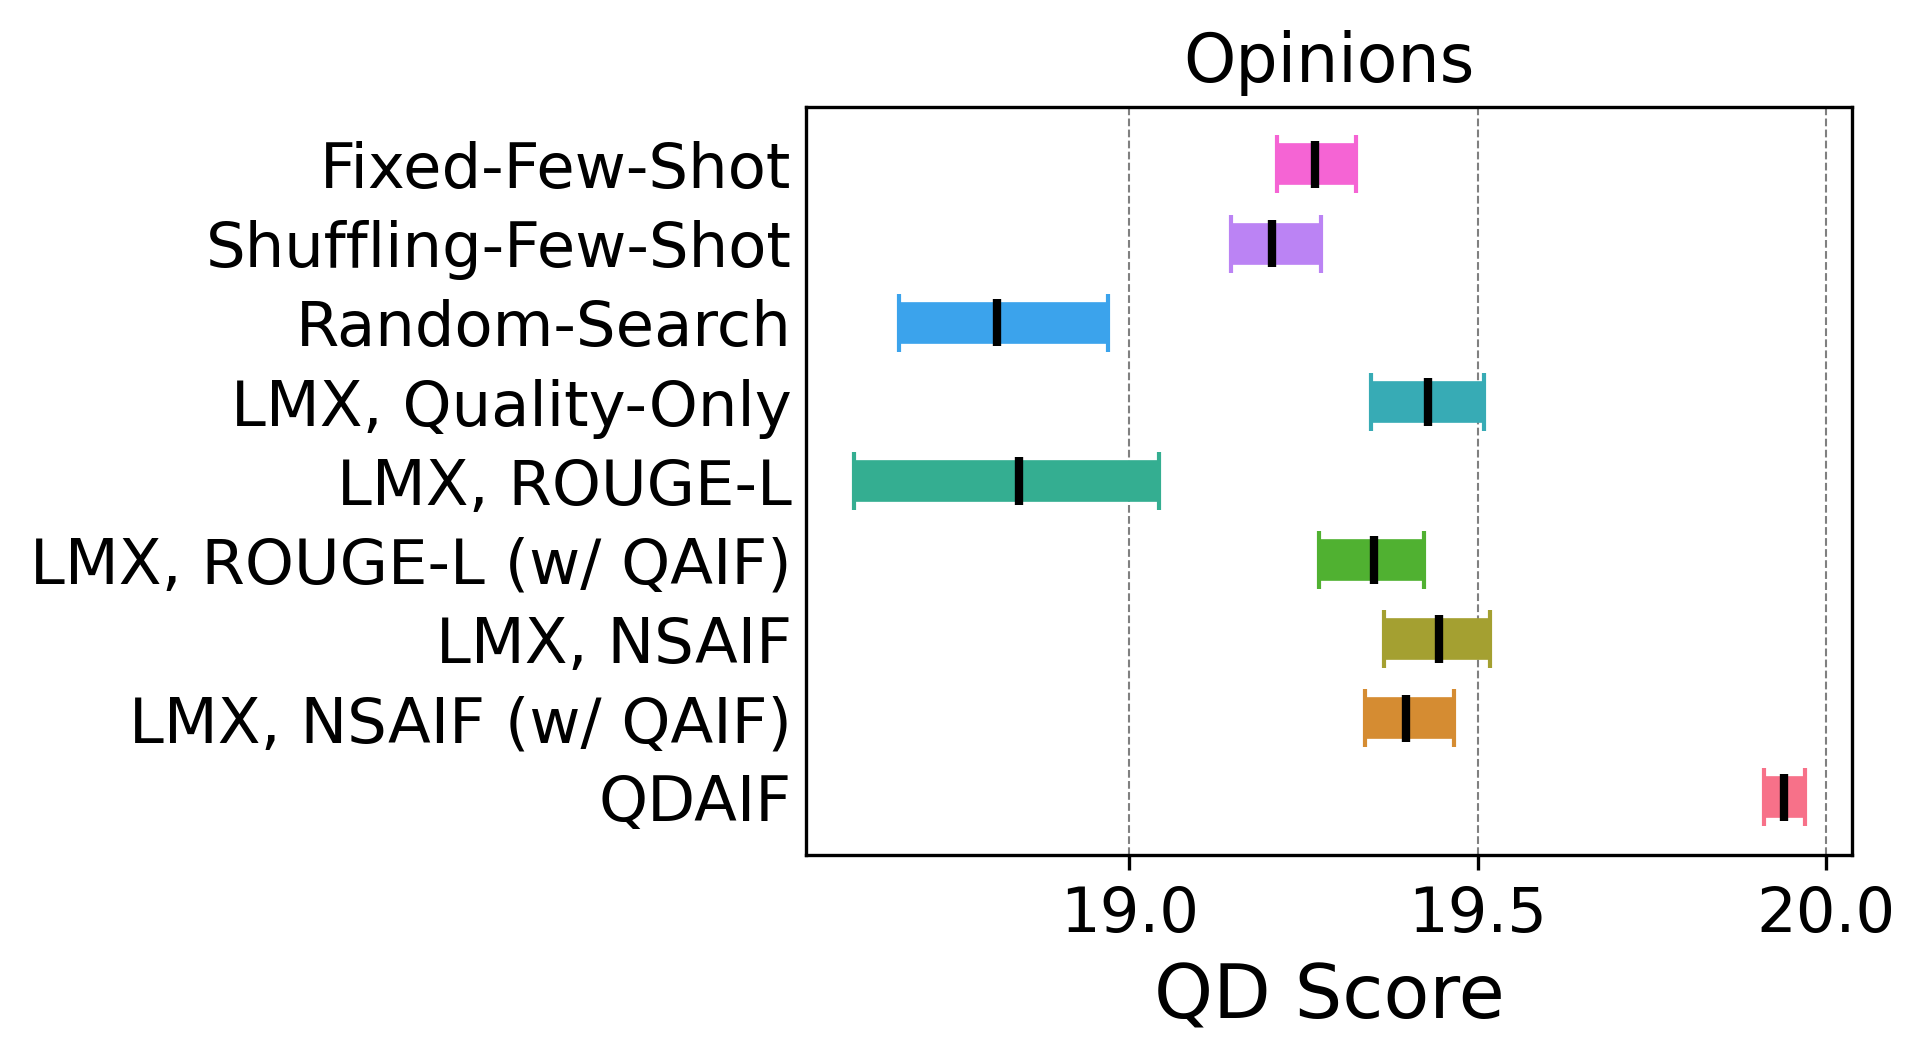
\includegraphics[height=0.119\textheight]{main_figures/extensions/extended_baselines_perf/qd_vs_non_qd_opinions.png}
    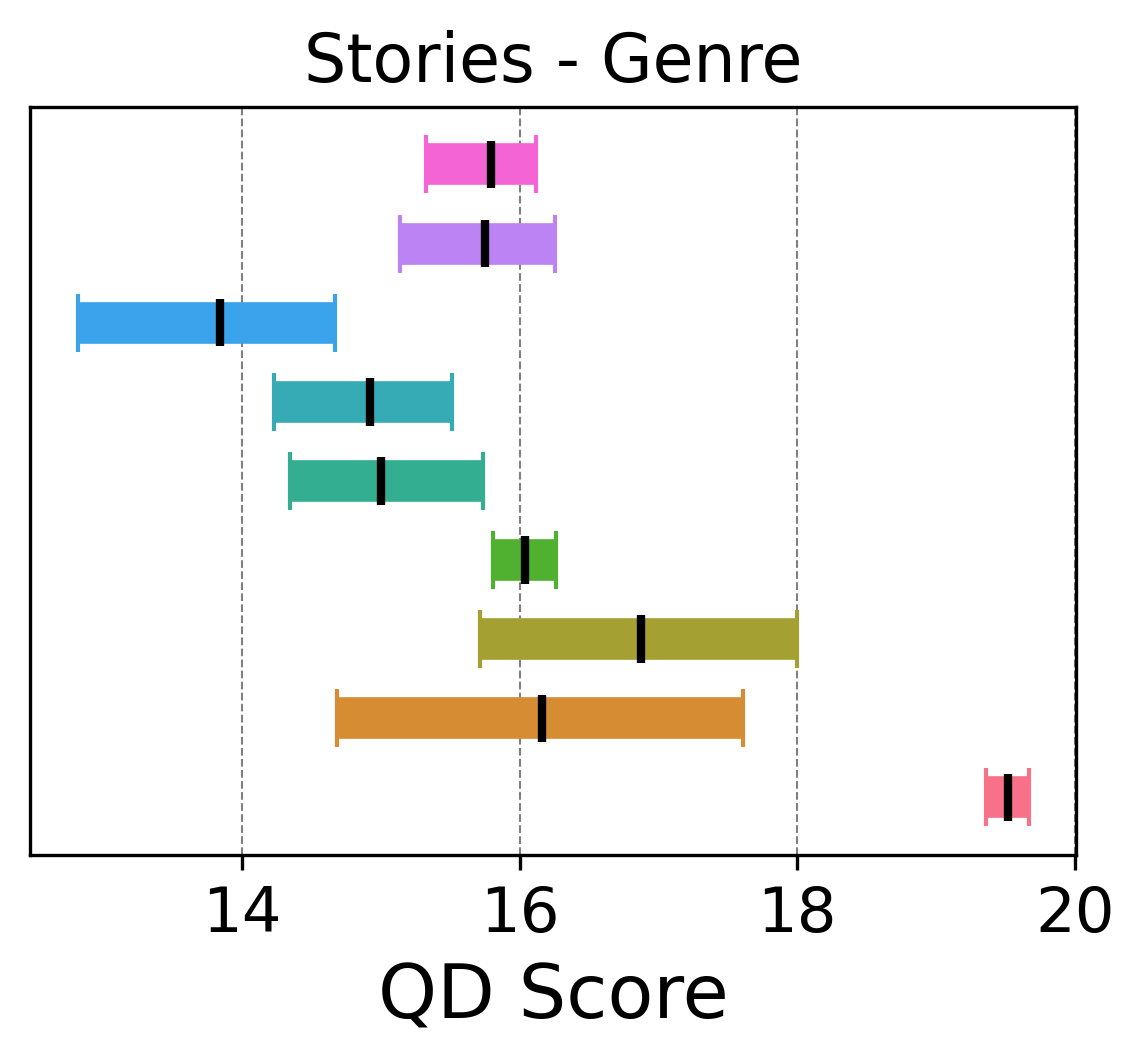
\includegraphics[height=0.119\textheight]{main_figures/extensions/extended_baselines_perf/qd_vs_non_qd_story_genre.png}
    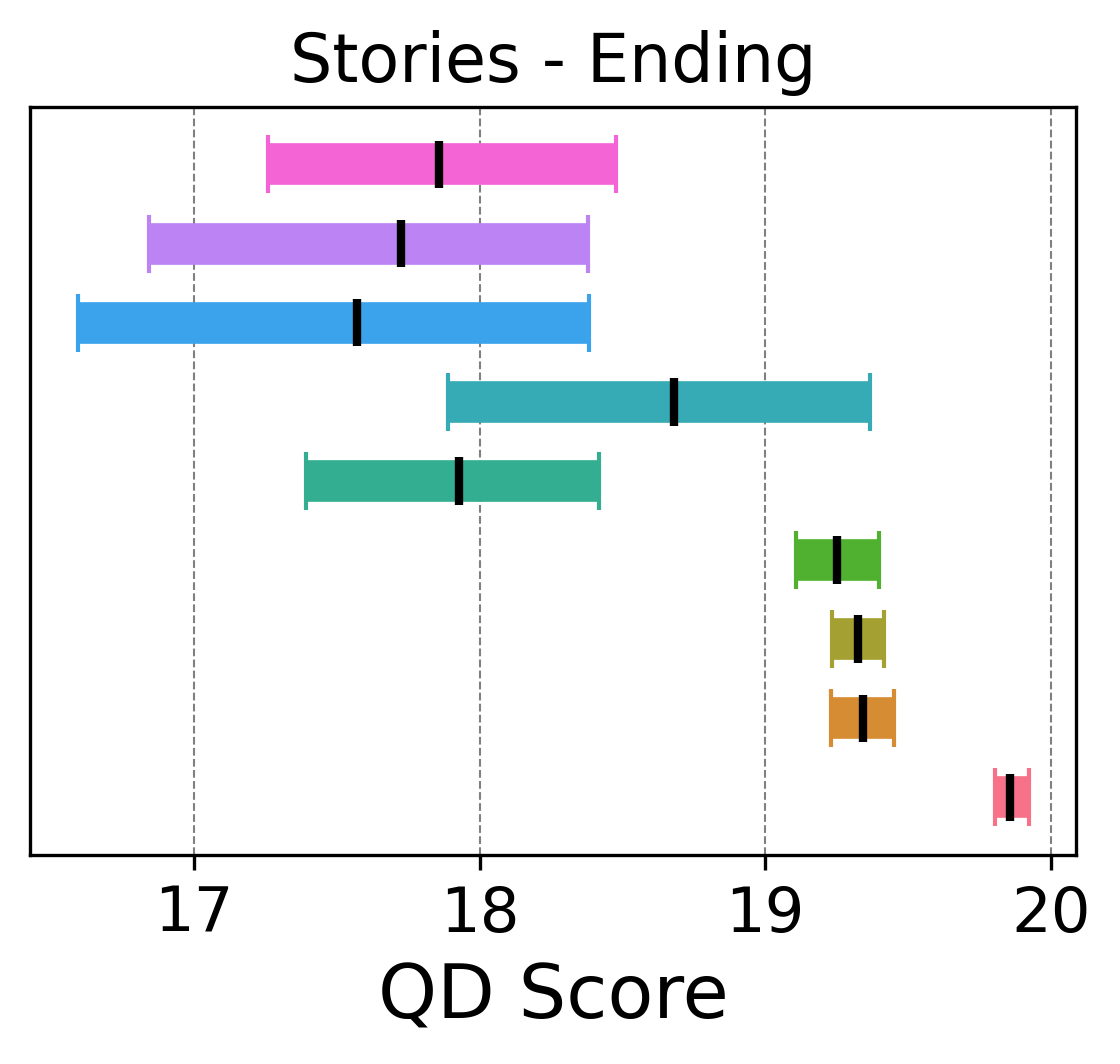
\includegraphics[height=0.119\textheight]{main_figures/extensions/extended_baselines_perf/qd_vs_non_qd_story_ending.png}
    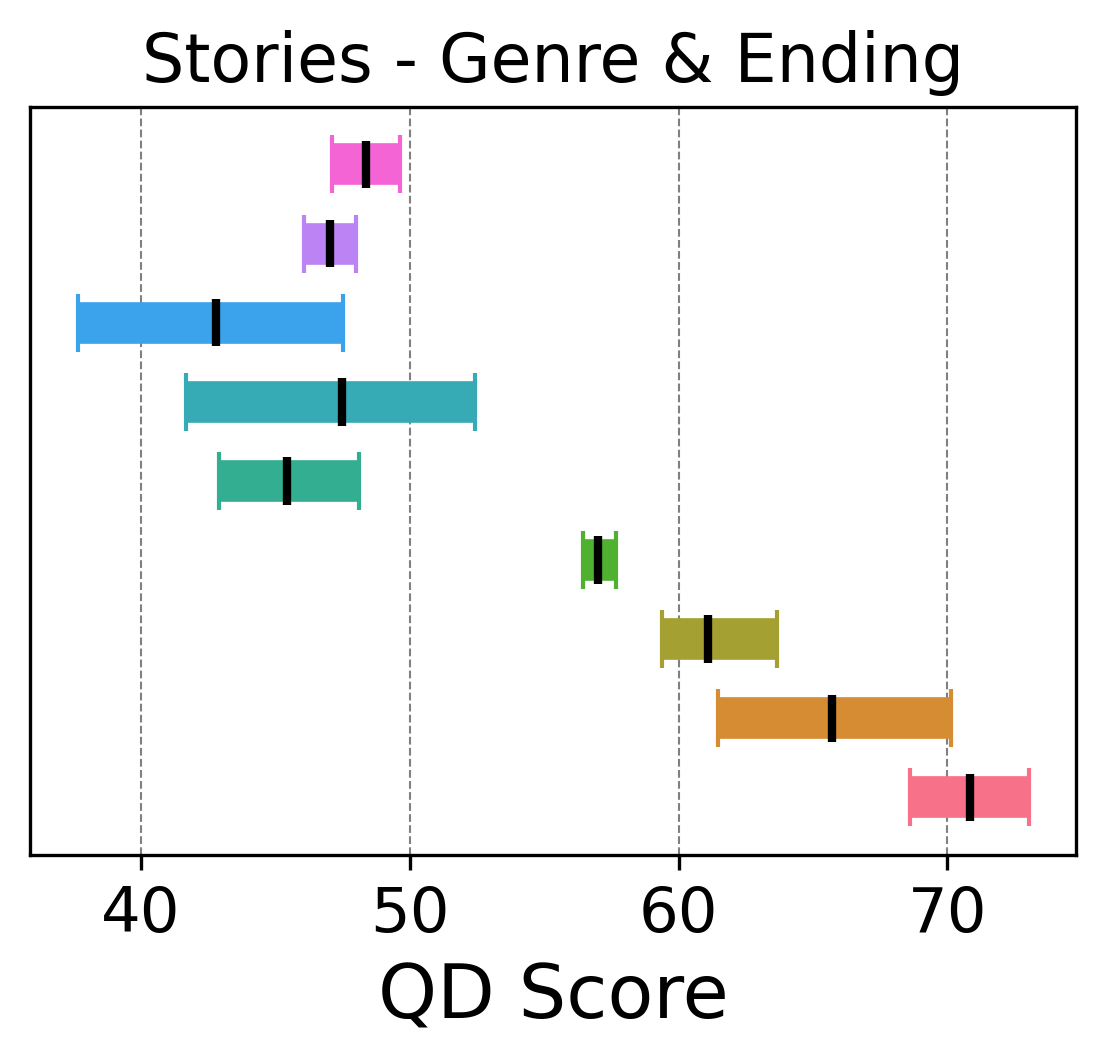
\includegraphics[height=0.119\textheight]{main_figures/extensions/extended_baselines_perf/qd_vs_non_qd_story_genre_ending.png}
    \vspace{-0.45cm}
    \caption{\textbf{QDAIF outperforms (diversity-seeking) baselines across domains in QD score and maintains high-performance across all domains}. Performance stats with mean bootstrapped 95\% CI, across 5 random seed runs. The maximum possible QD score is 20 (100 for 2D archive (4th plot)). The best-performing baseline in the \textbf{Stories - Genre and Ending} domain, \basesixq, does not consistently outperform other baselines in other domains, and has wide performance variability in two domains. Compared to \basefour, all the diversity-seeking baselines using NSAIF or ROUGE-L filtering (except \basefive) significantly outperform this baseline approach that optimizes for a single quality score objective.}
    \label{app:fig:extended_baselines_qd_score}
\end{figure}

\begin{figure}[ht]
    \centering
    % \hspace*{-0.8cm}
    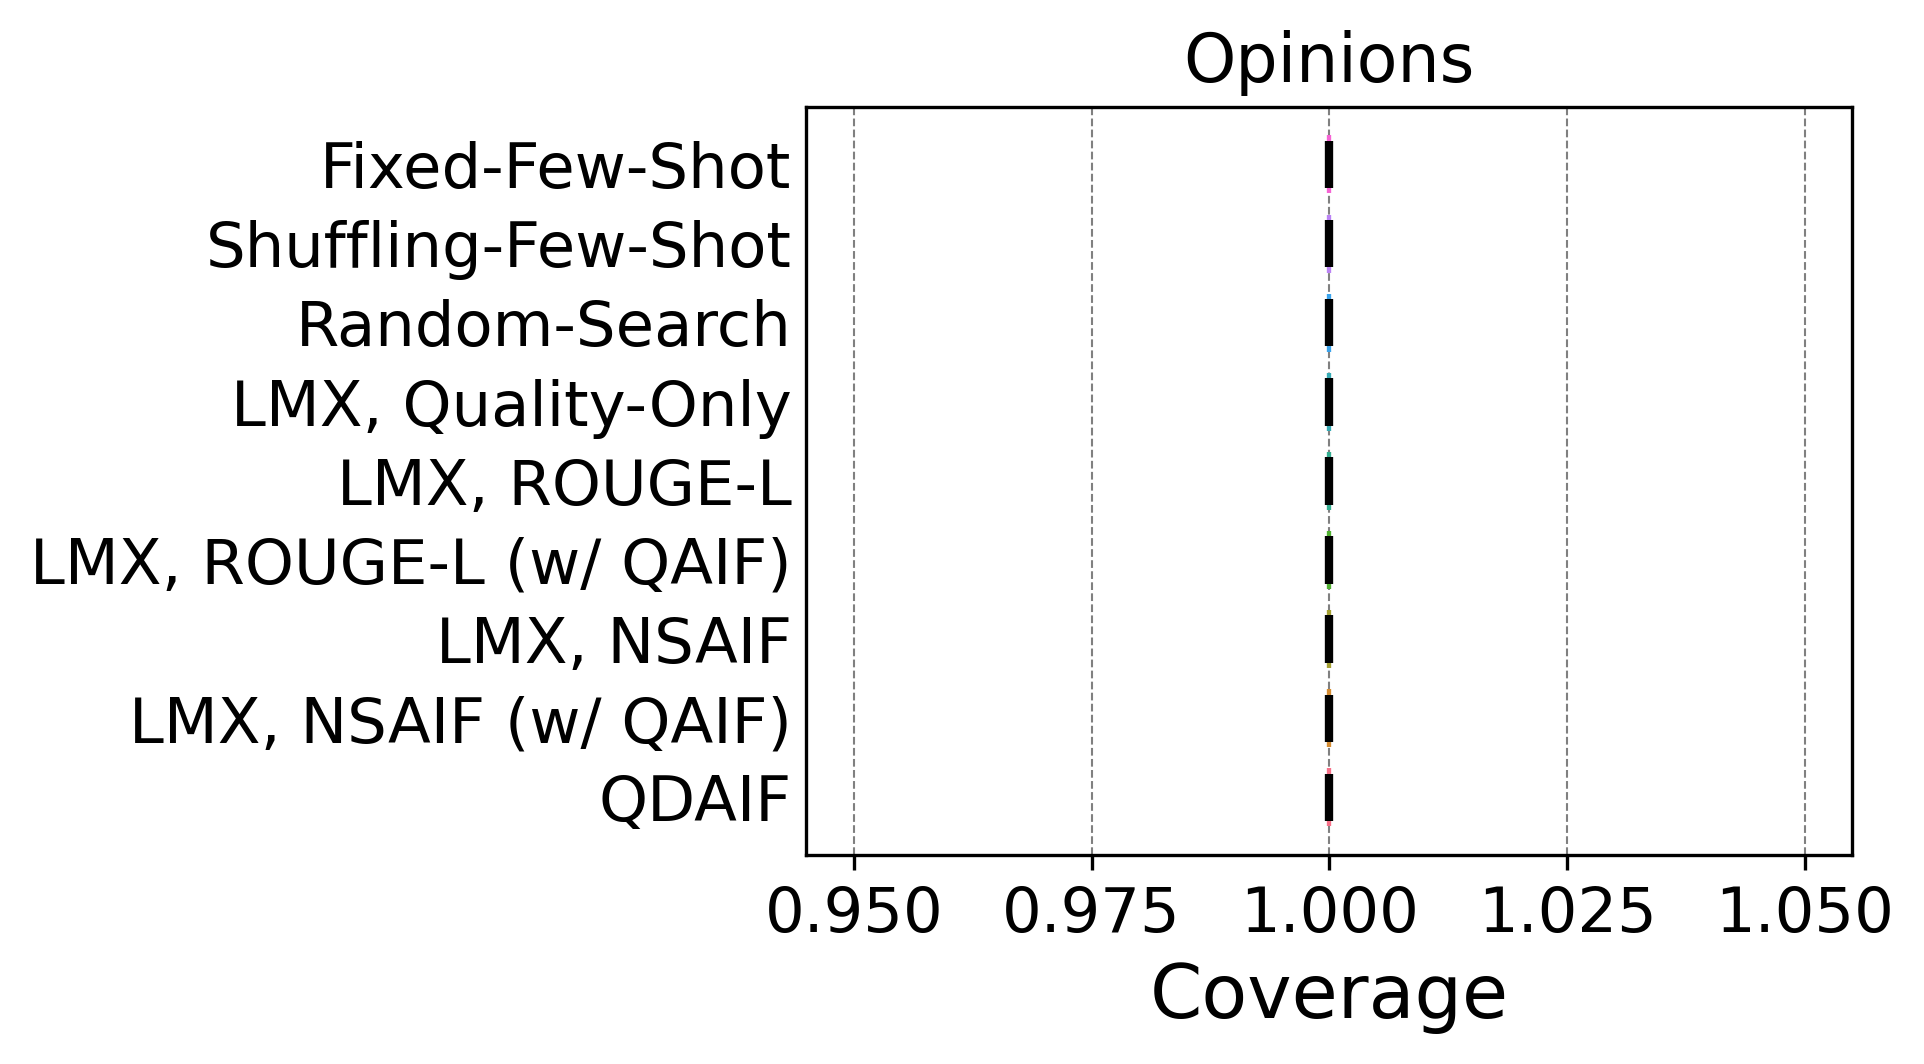
\includegraphics[height=0.119\textheight]{main_figures/extensions/extended_baselines_perf/qd_vs_non_qd_opinions_cov.png}
    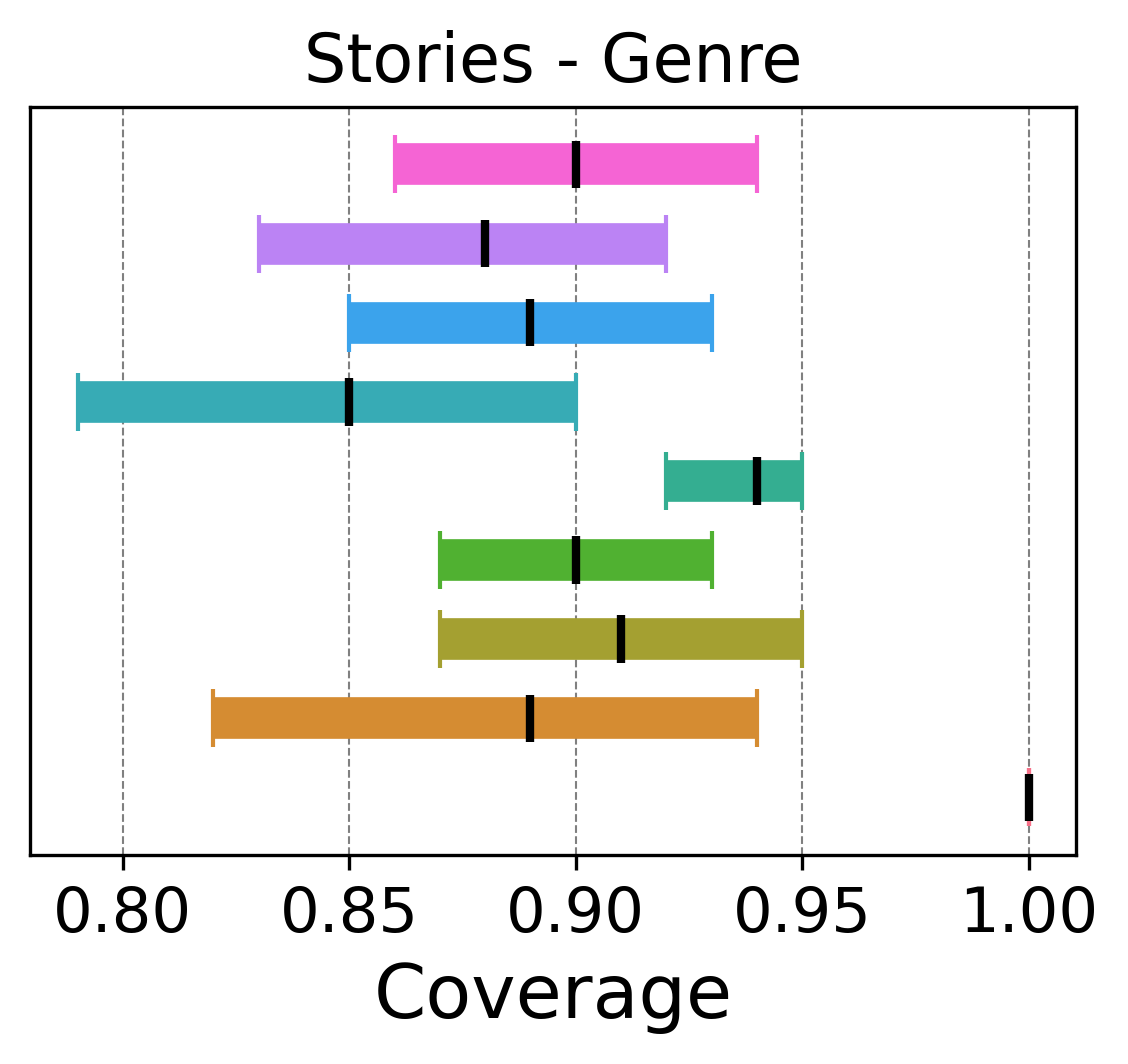
\includegraphics[height=0.119\textheight]{main_figures/extensions/extended_baselines_perf/qd_vs_non_qd_story_genre_cov.png}
    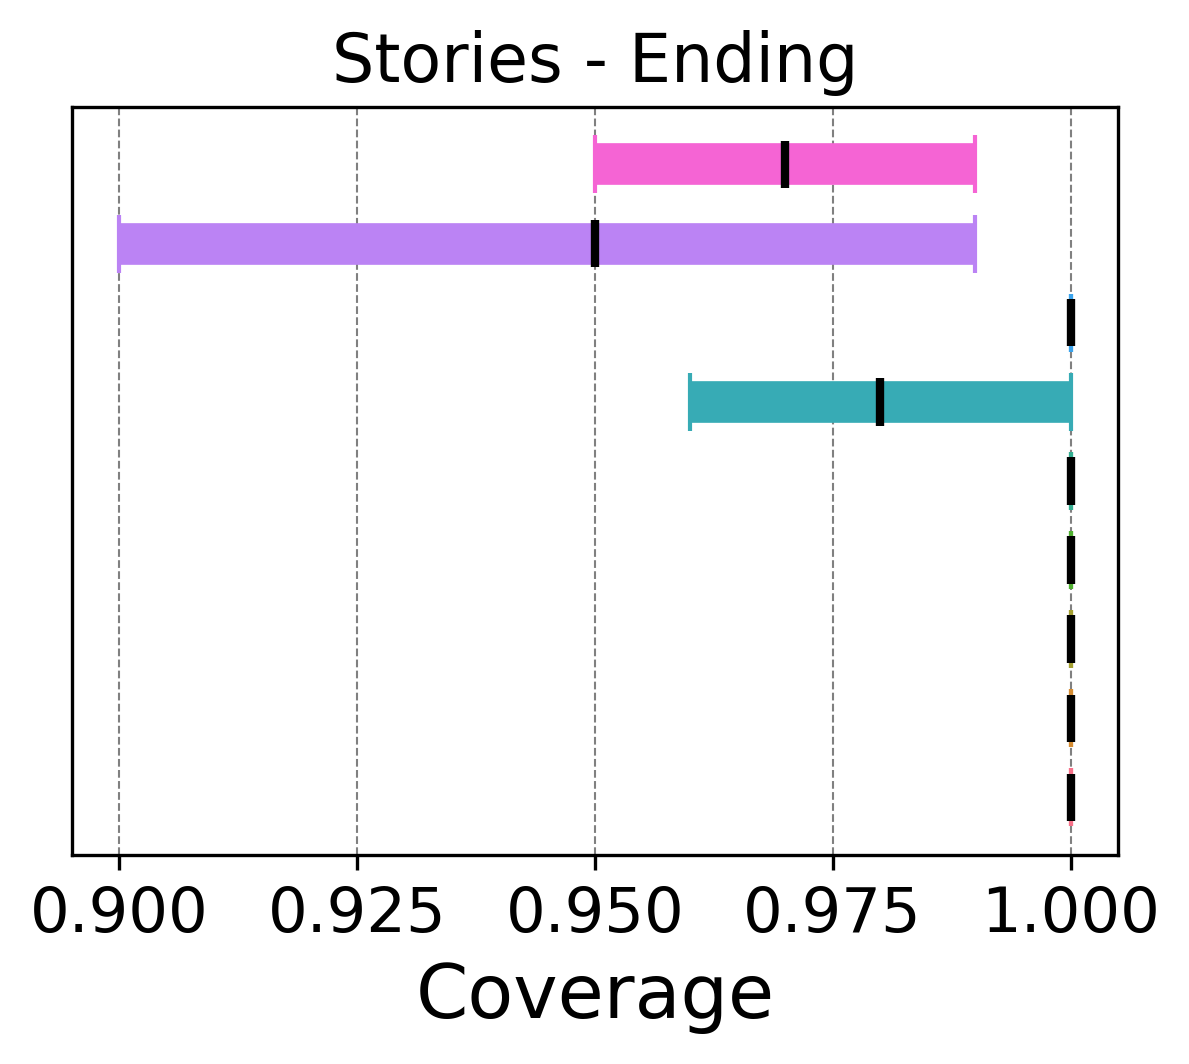
\includegraphics[height=0.119\textheight]{main_figures/extensions/extended_baselines_perf/qd_vs_non_qd_story_ending_cov.png}
    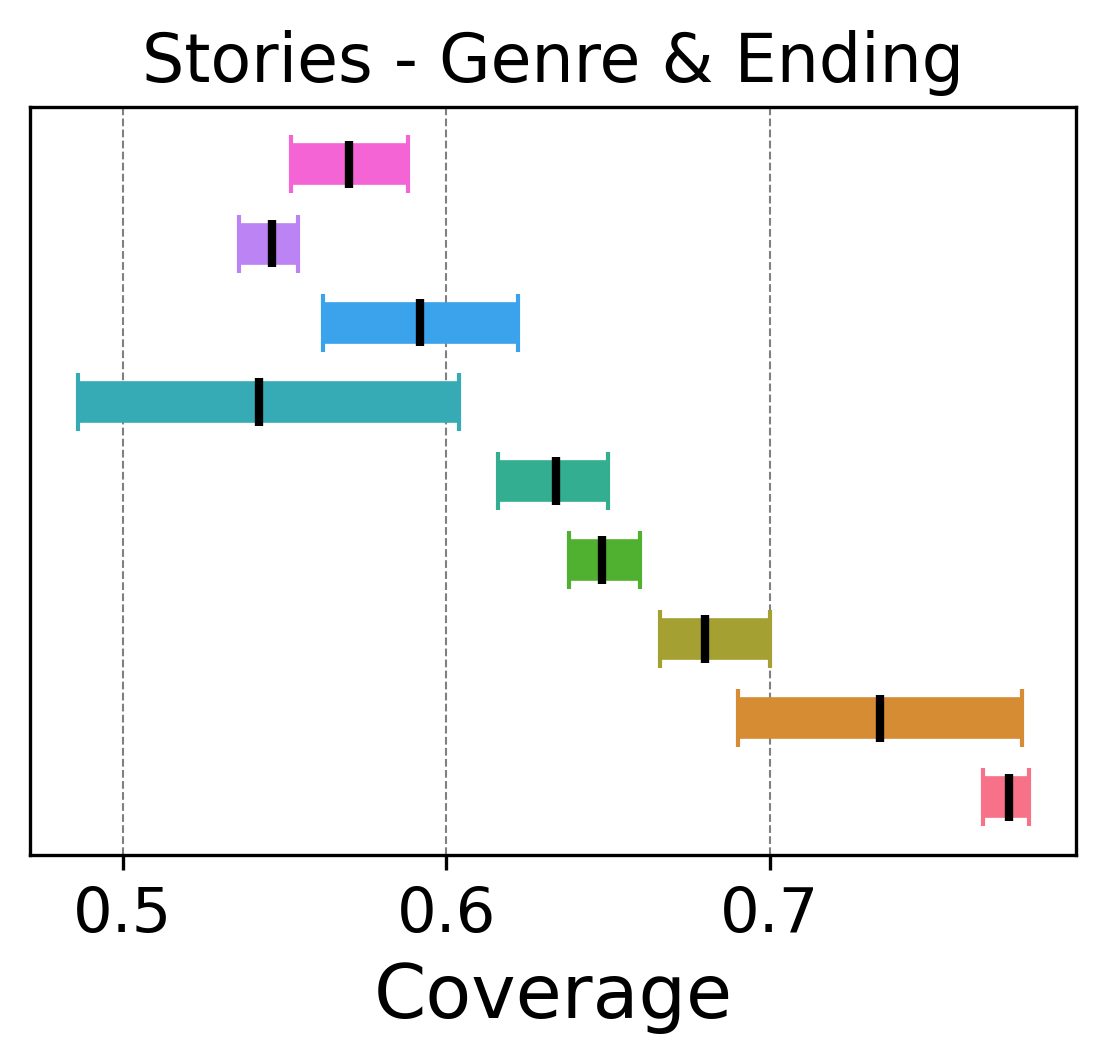
\includegraphics[height=0.119\textheight]{main_figures/extensions/extended_baselines_perf/qd_vs_non_qd_story_genre_ending_cov.png}
    \vspace{-0.9cm}
    \caption{\textbf{QDAIF more often outperforms (diversity-seeking) baselines in the percentage of available bins covered by solutions in all domains, such as Stories - Genre, and Stories - Genre and Ending}. Coverage stats with mean bootstrapped 95\% CI, across 5 random seed runs. The maximum possible coverage is 1. In some cases, methods achieve maximum coverage across all runs. Consistent high-coverage performance from QDAIF compared to the next best baselines in \textbf{Stories - Genre and Ending} (\basesix{} and \basesixq) suggests that evolving from high-quality solutions is important to improving solution diversity, in addition to diversity-seeking search (where \basefive{} also achieves higher coverage more often compared to non-diversity-seeking baselines.}
    \label{app:fig:extended_baselines_coverage}
\end{figure}

\begin{figure}[ht]
    \centering
    % \hspace*{-0.8cm}
    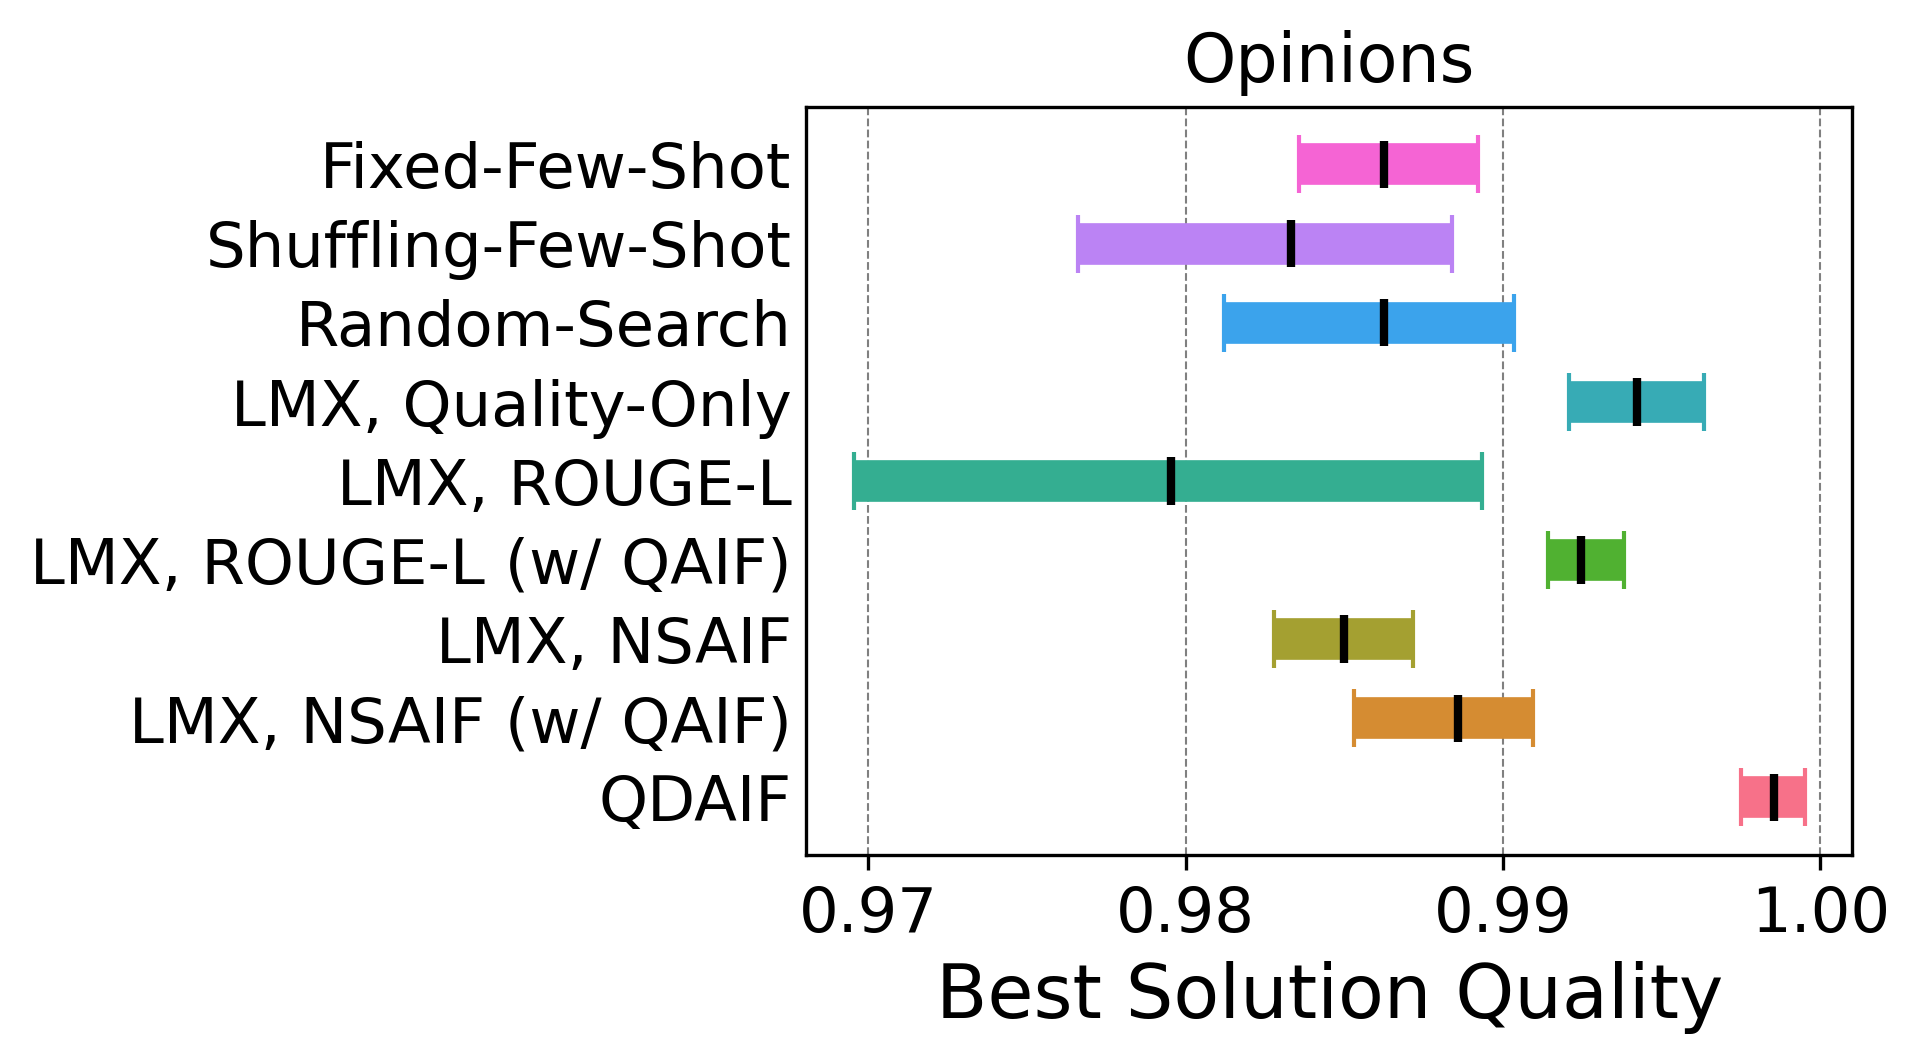
\includegraphics[height=0.119\textheight]{main_figures/extensions/extended_baselines_perf/qd_vs_non_qd_opinions_max.png}
    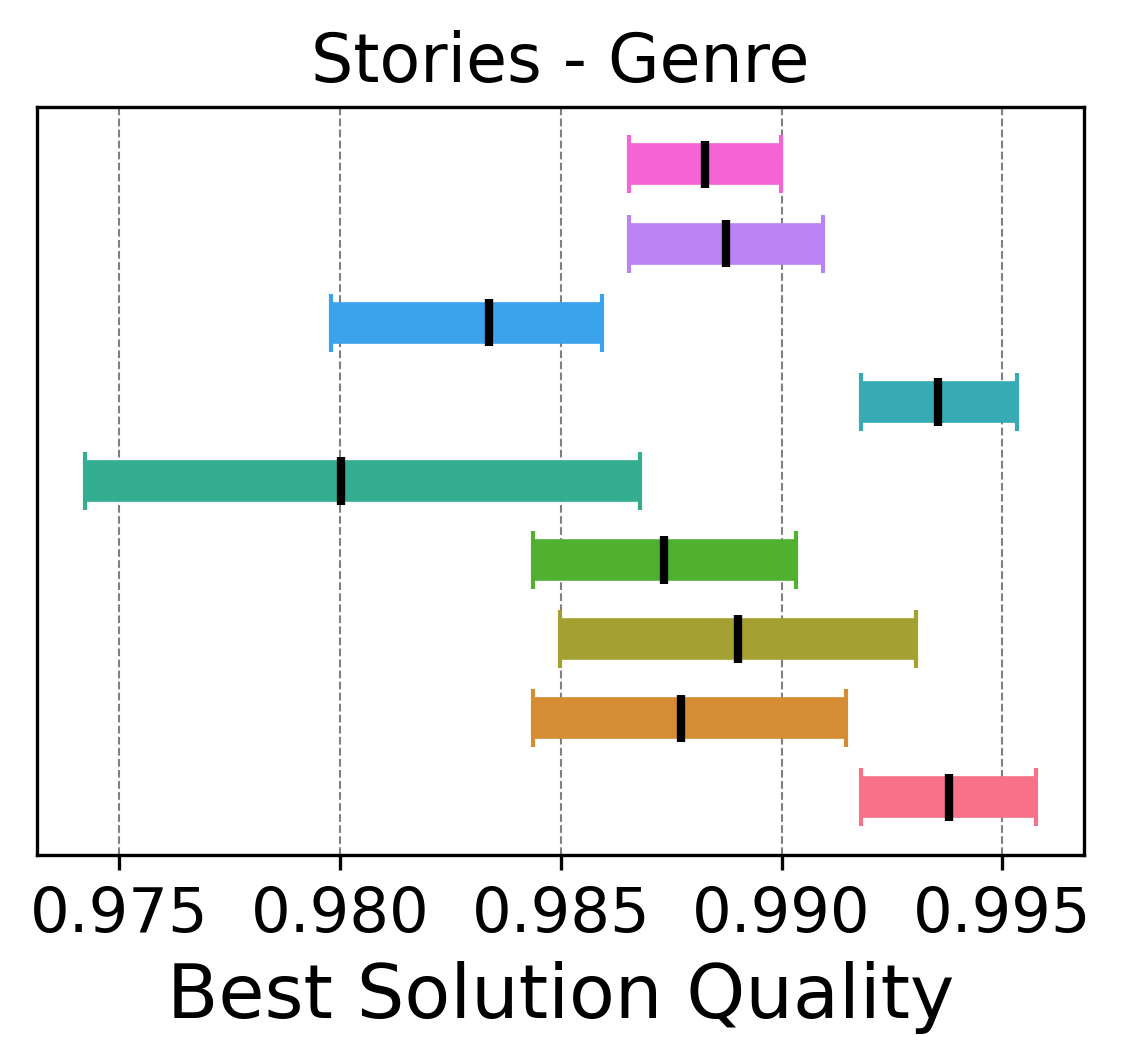
\includegraphics[height=0.119\textheight]{main_figures/extensions/extended_baselines_perf/qd_vs_non_qd_story_genre_max.png}
    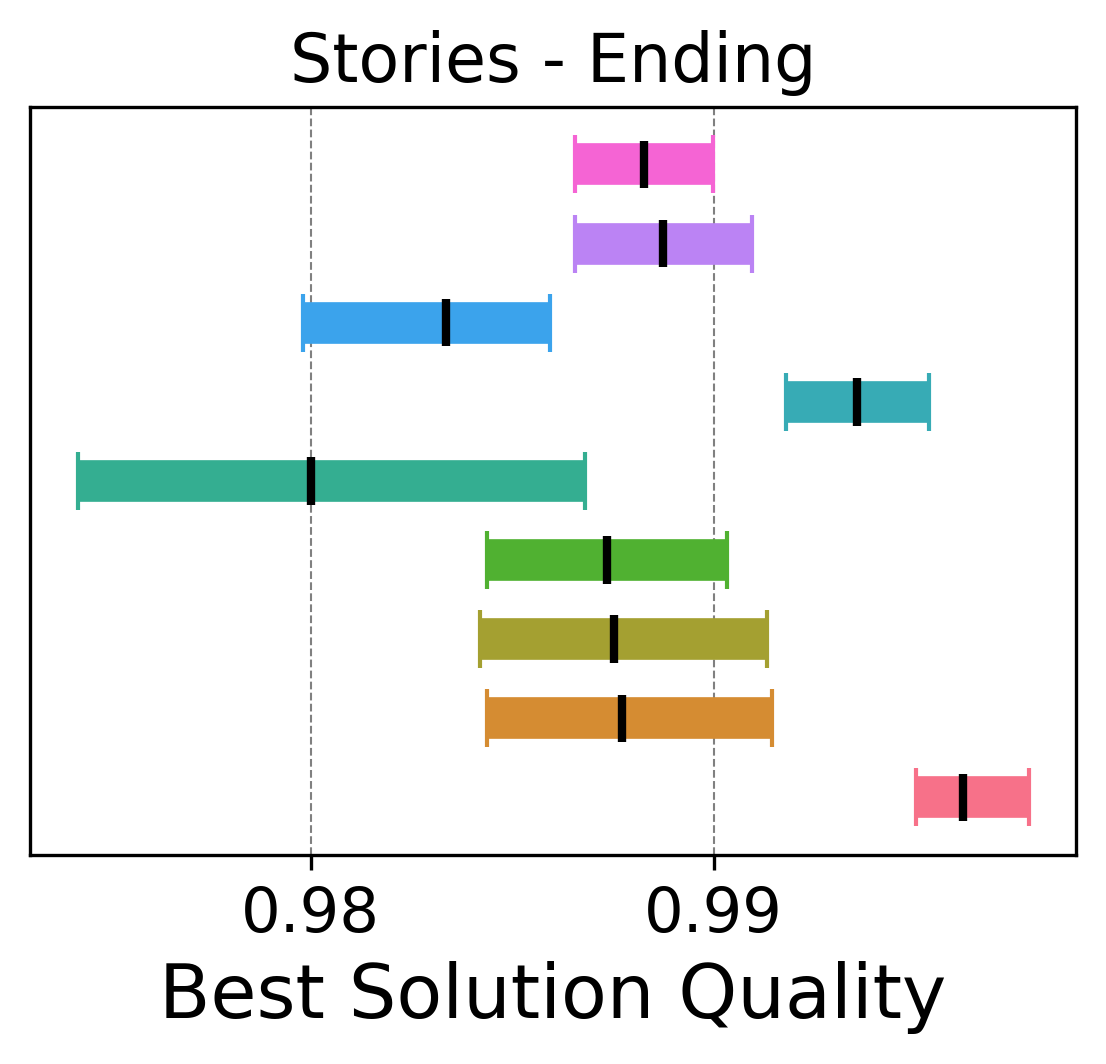
\includegraphics[height=0.119\textheight]{main_figures/extensions/extended_baselines_perf/qd_vs_non_qd_story_ending_max.png}
    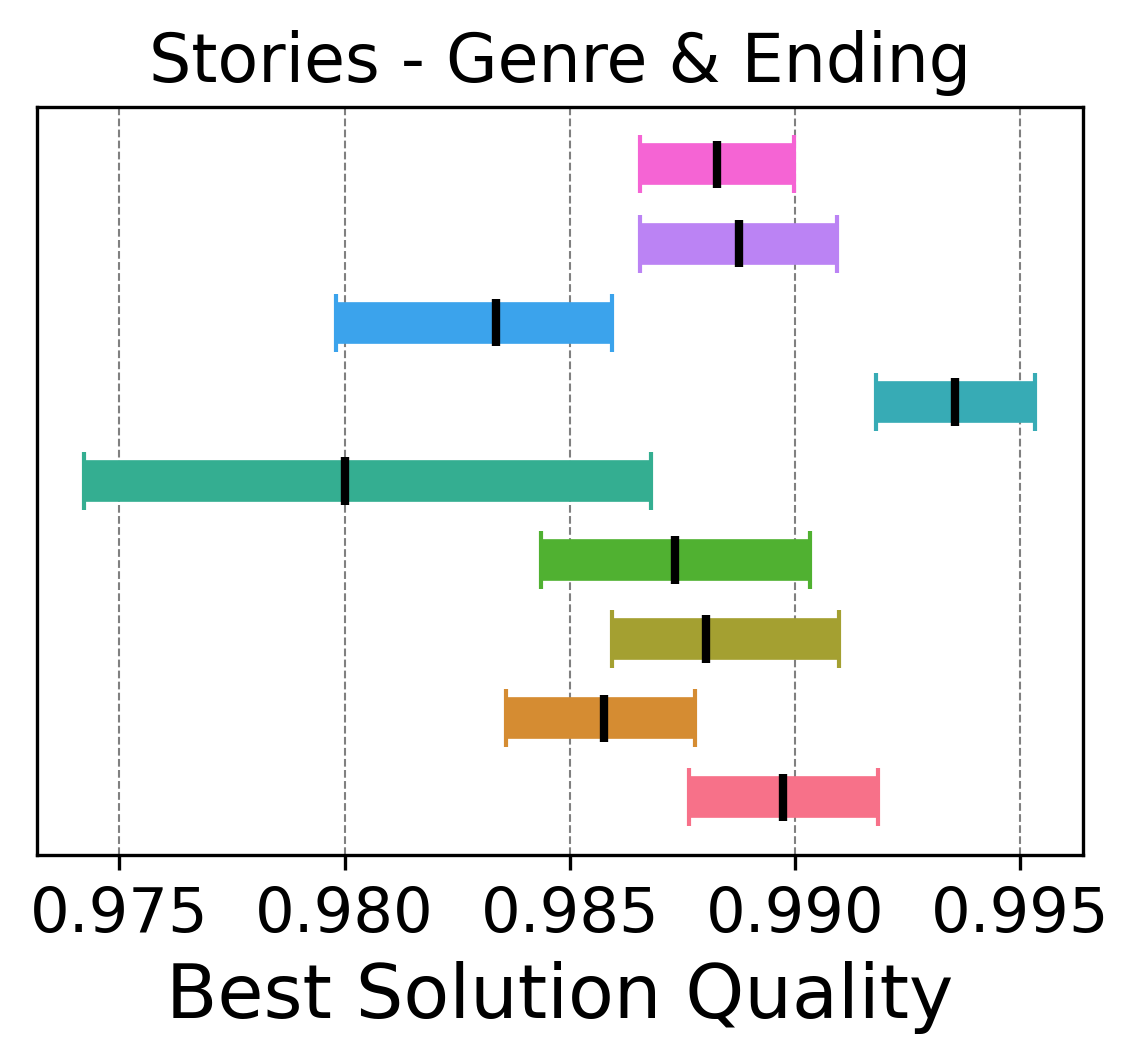
\includegraphics[height=0.119\textheight]{main_figures/extensions/extended_baselines_perf/qd_vs_non_qd_story_genre_ending_max.png}
    \vspace{-0.45cm}
    \caption{\textbf{QDAIF and \basefour{} both more often optimize for the quality of the best solution found overall}. Best solution quality stats with mean bootstrapped 95\% CI, across 5 random seed runs. The maximum possible quality score is 1. The addition of quality filters to \basefiveq{} and \basesixq{} is ineffective for significantly improving the best solution quality across runs compared to QDAIF. Still, \basefiveq{} is better compared to \basefive{} at finding higher-quality best solutions.}
    \label{app:fig:extended_baselines_max_fitness}
\end{figure}

\begin{figure}[ht]
    \centering
    % \hspace*{-0.8cm}
    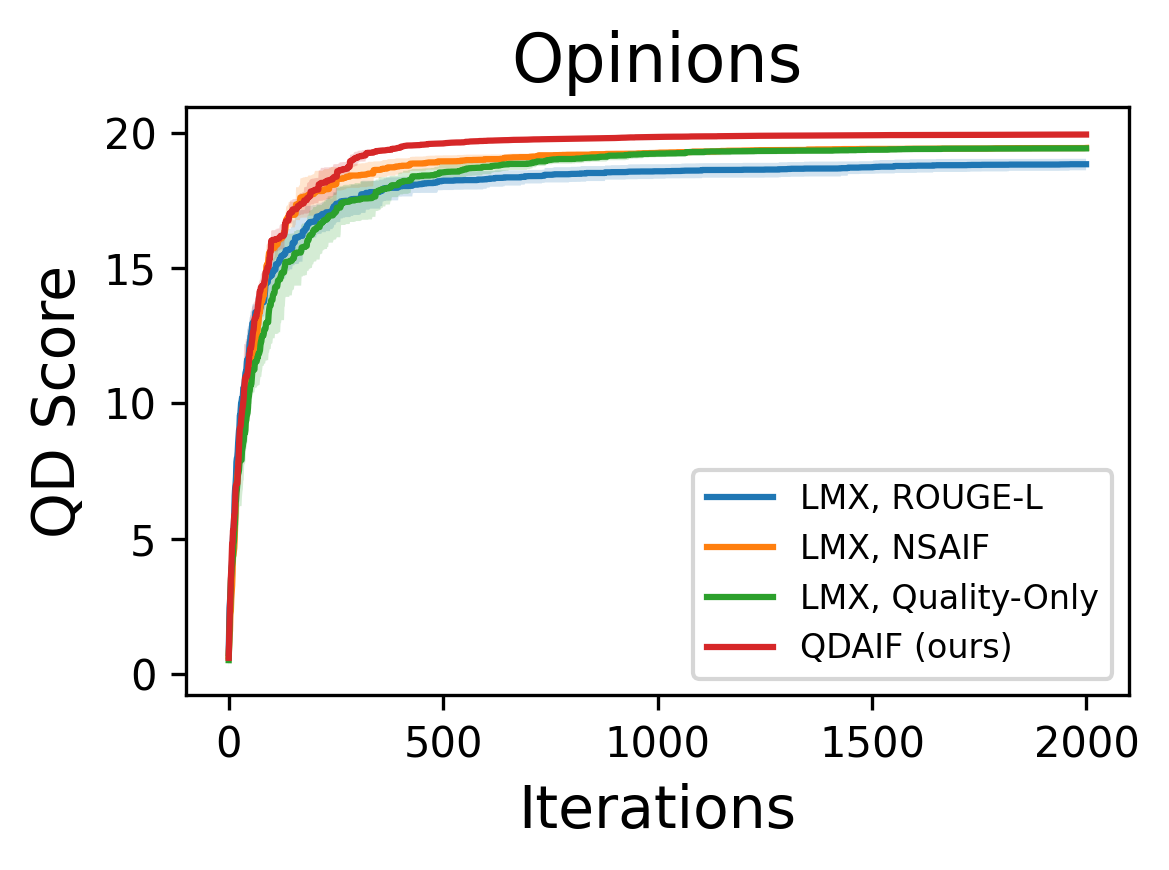
\includegraphics[width=0.49\textwidth]{main_figures/extensions/extended_baselines_line_plots/line_plot_opinions_div_only.png}
    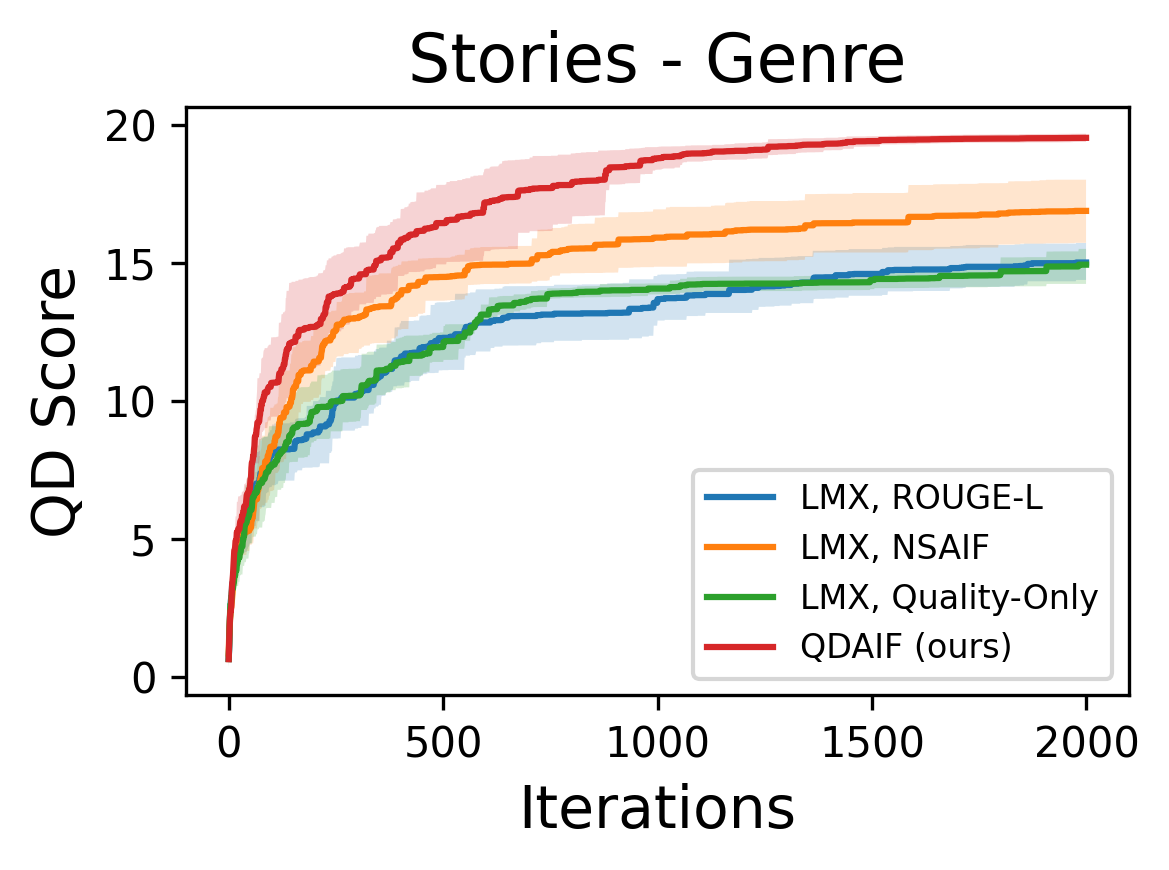
\includegraphics[width=0.49\textwidth]{main_figures/extensions/extended_baselines_line_plots/line_plot_stories_genre_div_only.png}
    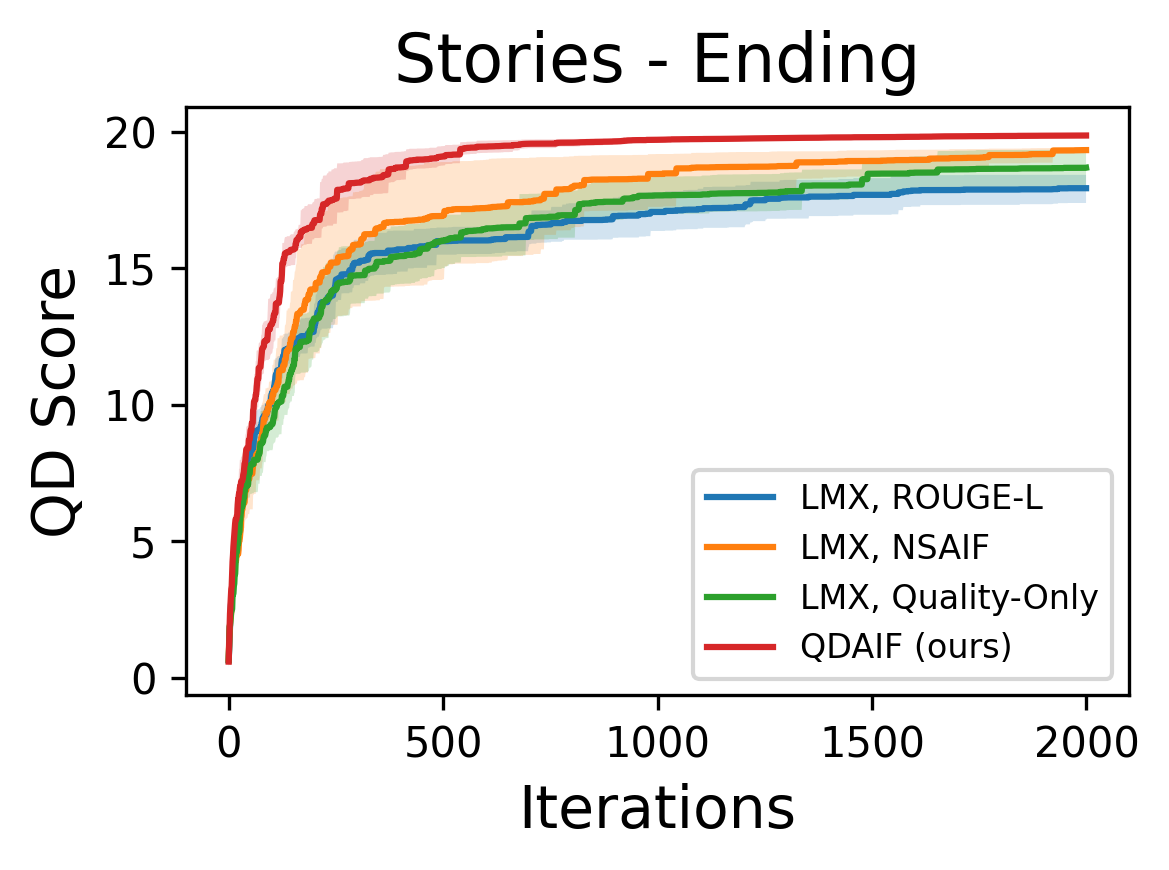
\includegraphics[width=0.49\textwidth]{main_figures/extensions/extended_baselines_line_plots/line_plot_stories_ending_div_only.png}
    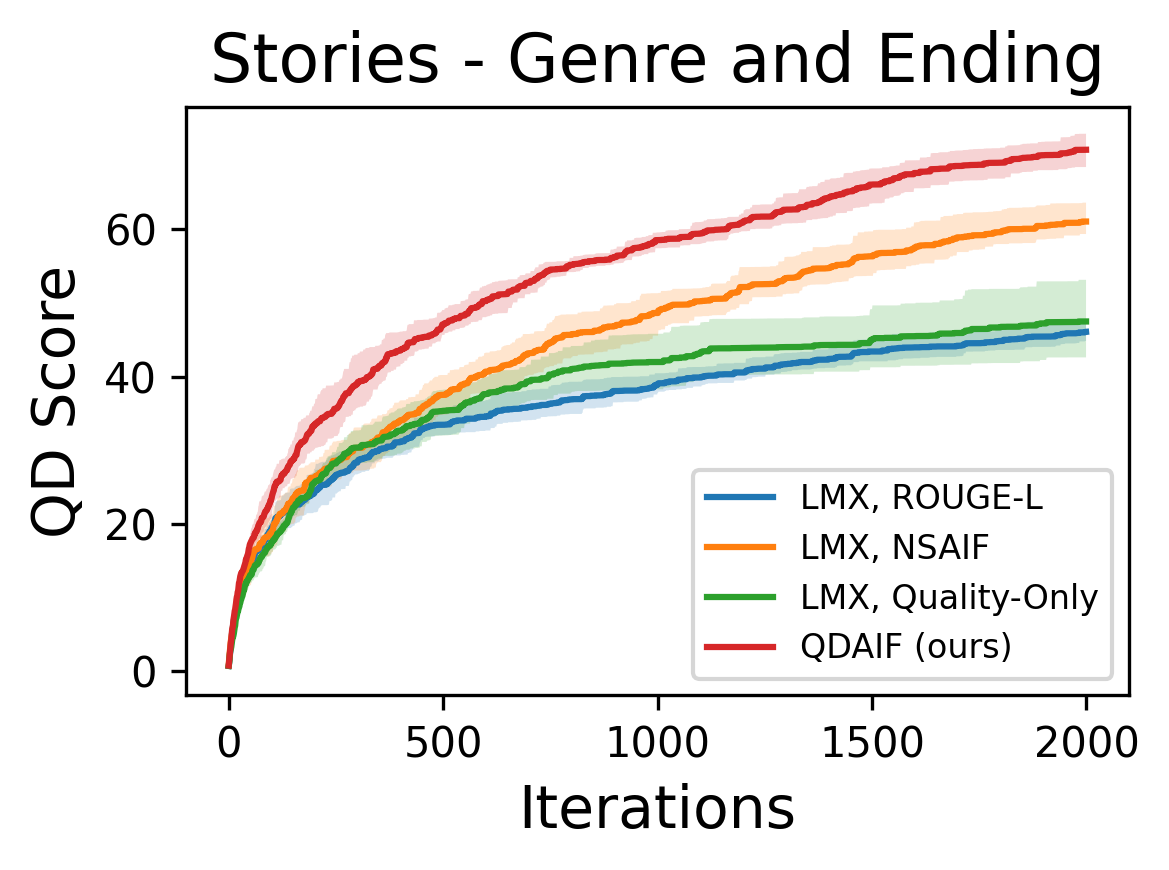
\includegraphics[width=0.49\textwidth]{main_figures/extensions/extended_baselines_line_plots/line_plot_stories_genre_ending_div_only.png}
    \vspace{-0.45cm}
    \caption{\textbf{QDAIF outperforms (diversity-seeking) baselines across domains in sample efficiency of QD score improvement}. Line plot stats with mean bootstrapped 95\% CI, across 5 random seed runs. The maximum possible QD score is 20 (100 for 2D archive (4th plot)). Additionally, \basesix{} succeeds in obtaining higher sample efficiency more often than \basefour, the single quality objective optimization method, without any optimization of the quality score objective.}
    \label{app:fig:extended_baselines_line_div_only}
\end{figure}

\begin{figure}[ht]
    \centering
    % \hspace*{-0.8cm}
    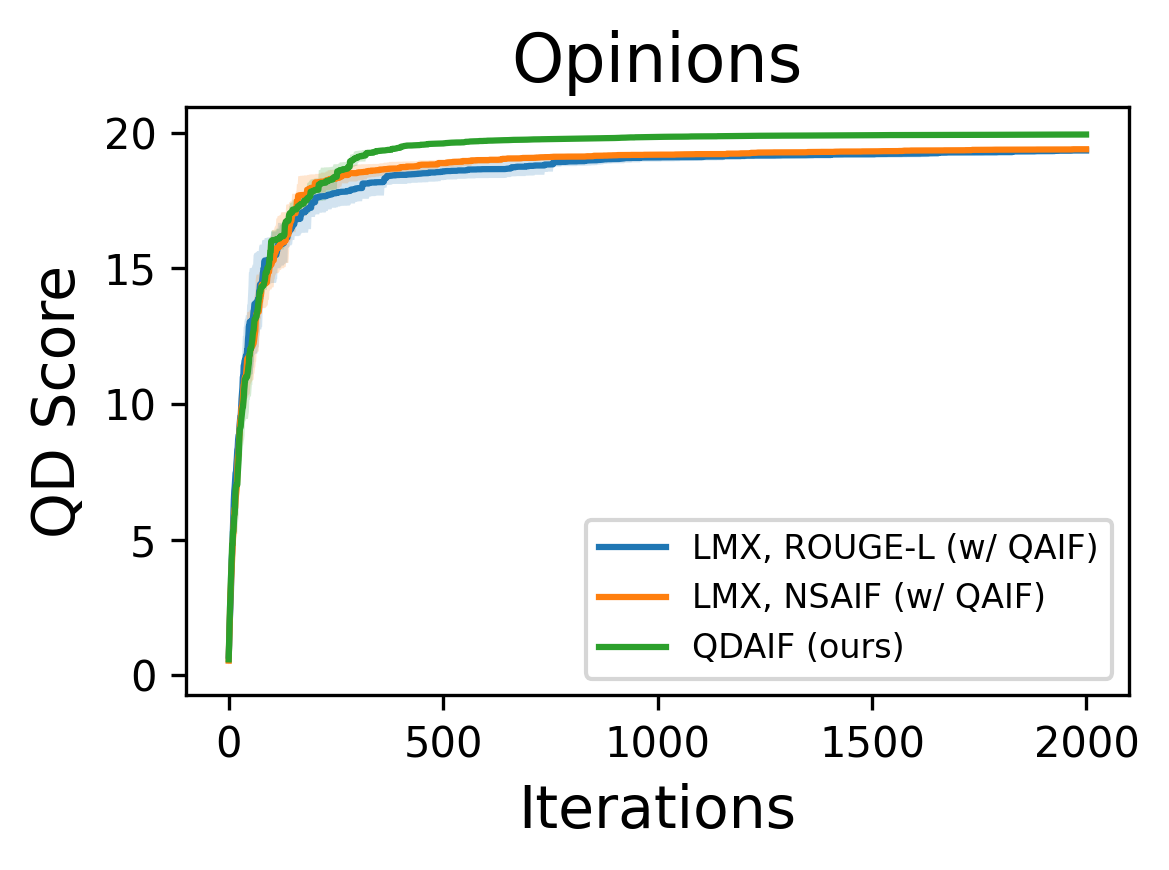
\includegraphics[width=0.49\textwidth]{main_figures/extensions/extended_baselines_line_plots/line_plot_opinions_qd.png}
    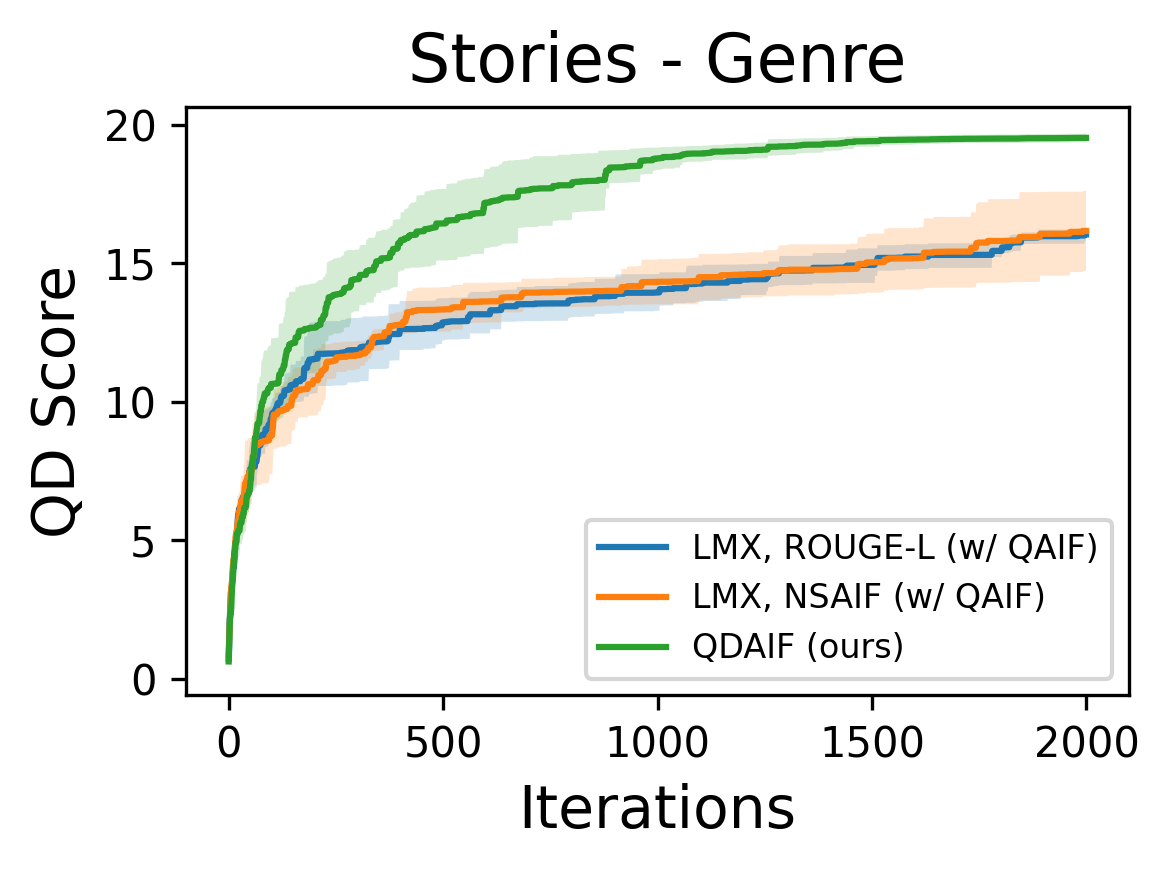
\includegraphics[width=0.49\textwidth]{main_figures/extensions/extended_baselines_line_plots/line_plot_stories_genre_qd.png}
    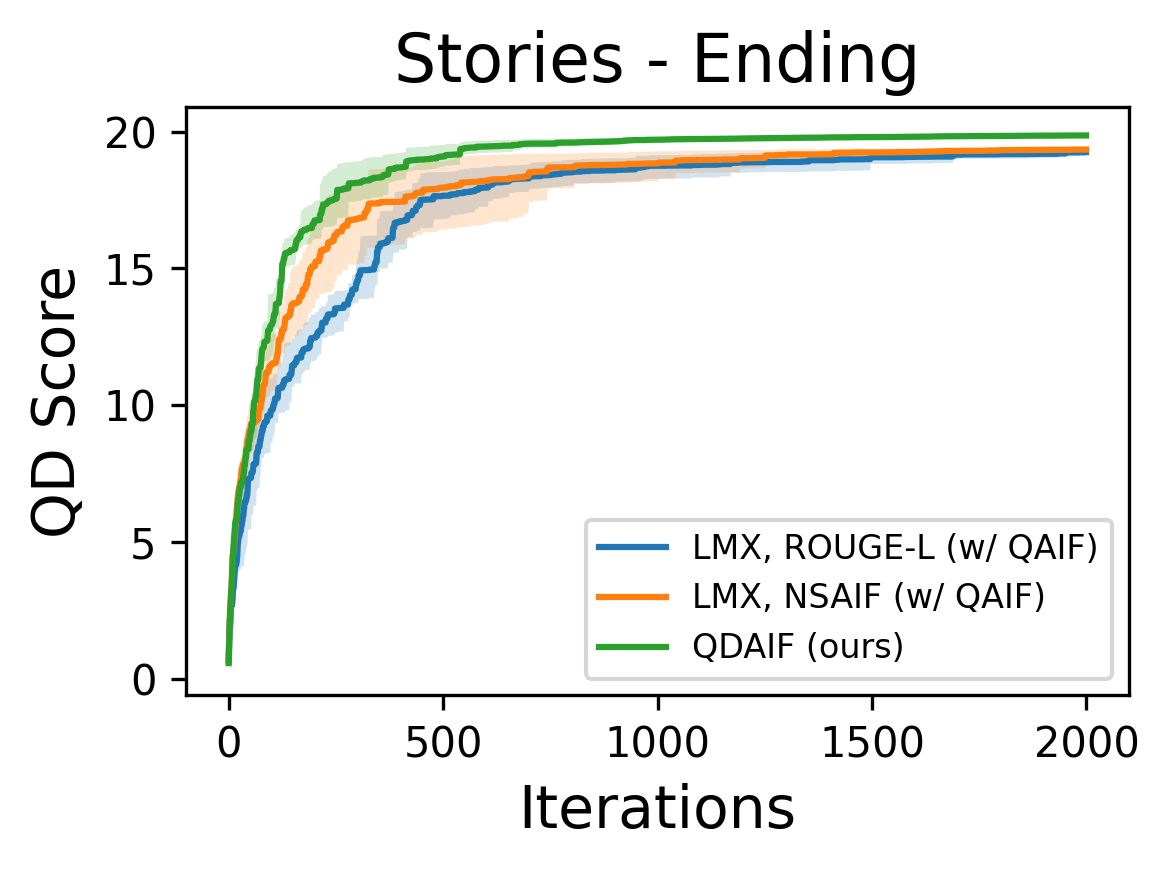
\includegraphics[width=0.49\textwidth]{main_figures/extensions/extended_baselines_line_plots/line_plot_stories_ending_qd.png}
    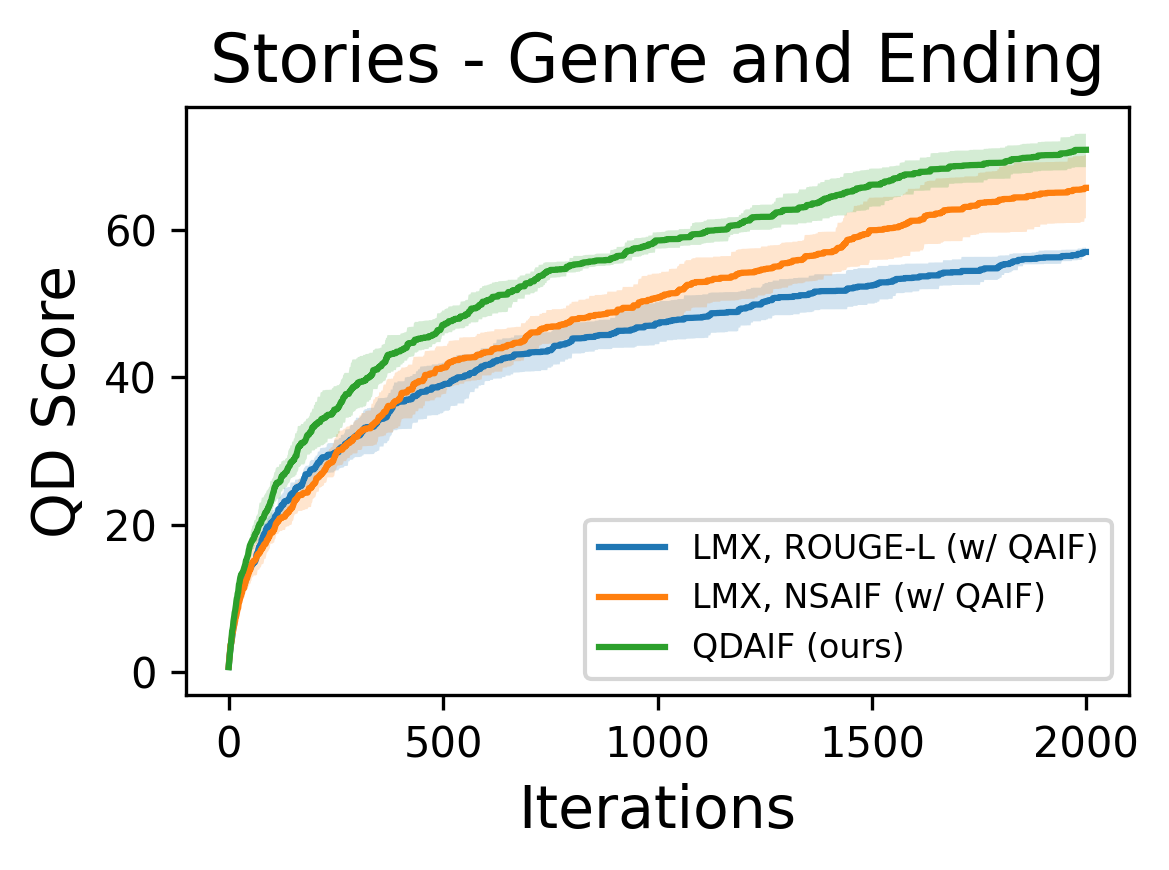
\includegraphics[width=0.49\textwidth]{main_figures/extensions/extended_baselines_line_plots/line_plot_stories_genre_ending_qd.png}
    \vspace{-0.45cm}
    \caption{\textbf{QDAIF outperforms (diversity-seeking, with quality control) baselines across domains in sample efficiency of QD score improvement}. Line plots with mean bootstrapped 95\% CI, across 5 random seed runs. The maximum possible QD score is 20 (100 for 2D archive (4th plot)). The improvement of QDAIF compared to other approaches aiming for diverse, high-quality solutions is significant in the \textbf{Stories - Genre} domain. In the \textbf{Stories - Genre and Ending} domain, \basesixq{} outperforms \basefiveq{} and is within the performance range of QDAIF in later iterations, but with lower sample efficiency in early iterations, and wider performance variability.}
    \label{app:fig:extended_baselines_line_div_with_qaif}
\end{figure}

\clearpage
\newpage
\subsection{Setup for Diversity-Seeking Baselines}\label{app:diversity_baselines_setup}
\basefive. Following \citet{wang2022self}, we set the threshold for the maximum allowed ROUGE-L similarity between generated texts and all texts in the prompt pool at any given time (from which few-shot examples are sampled for LMX generation) to 0.7, without limits on the prompt pool size. If the similarity exceeds this, the generated text is still logged for QD score evaluation, but rejected from being added to the prompt pool. Otherwise, the text is added to the prompt pool so that it can be used for LMX evolution during later samplings of few-shot prompts. The rest of the setup is comparable to QDAIF except for the MAP-Elites archive maintained by QDAIF.

\basesix. In line with the high-level implementation of NS described in \citet{lehman2008exploiting}, we implemented the novelty (diversity-based) measure in the same way that QDAIF defines diversity measures - as the diversity attribute defined by the AI feedback axis (or axes) in the range [0, 1], with an additional Euclidean distance-based measure between the diversity attribute of the generated text, and existing texts in the prompt pool. Novelty is computed by measuring the mean distance between the diversity attribute values of the generated text, and their $k$ nearest neighbors in the prompt pool (with respect to the diversity attributes of the neighbor texts). We keep $k$ to be 15, as was tested in the original NS implementation. Similar to NS, the novelty score is compared to a novelty threshold (initially 0.05 in all \basesix{} runs, the distance width between adjacent bin ticks for a unit range with 20 uniform bins); if the novelty of the generated text is higher than the threshold, it gets accepted into the prompt pool for evolution with LMX, otherwise, it is logged for evaluation of performance results but rejected from the prompt pool. We apply a dynamic adjustment of the novelty threshold, following NS, and define it so that the threshold is multiplied by 1.05 (increased) if 3 solutions in a row were accepted to the prompt pool within any iterations window, or multiplied by 0.95 (decreased) if 21 solutions in a row were rejected from the prompt pool during the search.

In consideration of the non-linear calibration of AI feedback models in evaluating texts (cf. \cref{main:binning}), we apply a piecewise linear transformation to the original diversity attribute value from AI feedback evaluation of diversity (that lies along an axis discretized by non-uniform binning) so that it lies instead along an axis discretized by uniform bins while preserving the number of bin intervals. For example, in our 20-bin setting, the input value 0.9975, which lies between bin ticks 1, and 0.995, would be transformed to an output value of 0.975, and the input value 0.35 (between bin ticks 0.5 and 0.2) would be transformed to an output value of 0.475. This enables novelty to be computed using Euclidean distances while preserving the nature of AI feedback model non-linear calibration in distinguishing subjectively similar solutions from diverse solutions. Additionally, this keeps the definition of diversity consistent and fair with the setup of diversity measures for evaluation (in QDAIF iterations, and for baseline performance comparisons). The number of bin intervals defined for the piecewise linear transformation is the same as the number of intervals set as default across the \textbf{Opinions} and \textbf{Stories} domains (20 for 1D archives, 10 for 2D archives).

\textbf{Quality AI Feedback Filtering.} We implemented and assessed variants of the above baselines, \basefiveq, and \basesixq, by adding a simple quality filter for accepting generated texts to prompt pools, based on quality AI feedback defined in the respective creative writing domains. This involves an additional step in each baseline method immediately after the diversity criteria assessment of solutions, where generated texts must also have quality score values above a minimum threshold before being added to the prompt pool. Thus, these variants become similar to QDAIF methods, where they aim for diverse, high-quality solutions. These baselines differ from our default QDAIF method with MAP-Elites in that the minimum quality thresholds are not a function of the quality of best solutions across individual bins, but are arbitrarily defined, to constrain the prompt pool to satisfy a minimum criterion for quality, as was introduced previously for diversity-seeking methods in \citet{lehman2010revising}. This would make the quality improvement process of solutions across all bins less sample-efficient. We define this simple quality threshold for the baselines to be fixed at 0.8, closer to the upper bound of the full quality range [0, 1]. This was determined based on the intuitions of the results from the human evaluation study we conducted (cf. \cref{fig:quality_vs_fitness} in \cref{app:human_study_setup}), where a quality value of 0.8 from AI feedback corresponds to a generally high human feedback Likert (quality) score. As done in \basefour, these baselines (with quality filtering) limit the size of the prompt pool to be up to 100.


\clearpage
\newpage
\subsection{On Automatically Expanding Archive Dimensions}\label{app:expanding_dim}
Prior work in QD, as described in \cref{main:qd_background}, often relies on diversity measures that are designed and manually defined at the start of the search. One existing approach for more automatic QD search without supervised (defined) measures of diversity is to use unsupervised learning to represent diversity without relying on ground truth measures \citep{cully2018hierarchical,cully2019autonomous,grillotti2021unsupervised,wang2023diversity,ding2023quality}. Such unsupervised approaches do not embody any complex prior of what humans find interesting about diversity; an alternative approach would be to query capable LMs about what dimensions of diversity are interesting or important for a particular domain. In this way, semantically-rich axes of diversity could be automatically generated (and could then be evaluated automatically as well through other LM calls, as in QDAIF).

Given the advances in foundation model capabilities, we could reasonably prompt LMs (such as GPT-4 \citep{openai2023gpt4}) to come up with new axes of diversity in a more automated pipeline potentially while search is running - by giving it a description of the user’s search problem, and existing diversity axis being searched through (i.e. the existing AI feedback diversity prompt(s)), we could ask the LM to give us a different, previously unexplored diversity axis and define a new AI feedback prompt that can be added to the MAP-Elites evaluation. For example, in the \textbf{Poetry} domain, we could ask the LM to generate multiple diverse aspects of poetry (e.g. “Genre” and “Tone” as studied in the presented experiments), and also come up with diverse categories defining this search space for QDAIF to search through with MAP-Elites. The effectiveness of this kind of approach has not been studied thoroughly in prior works, especially on the question of whether or not expanding the dimensions of diversity during the search can meaningfully improve diversity in resulting solutions towards increasingly broader definitions of diversity.

\textbf{Setup.} We took a step in the direction of automating the definition of diversity axes, where we analyzed the effectiveness of creative search for solutions when we expand the dimensions of diversity axes during an intermediate iteration of an existing search, with performance measured in terms of improving the QD score (for a given ground truth, higher-dimensional search space). We tested this approach in the \textbf{Stories - Genre and Ending} domain, compared the performance between variations in methods with QD score (out of 100) as done in other experiments, and compared the following setups: 2D Archive Search (apply QDAIF with the full 2D diversity axes defined), 1D Archive Search (apply QDAIF with only a 1D diversity axis defined, done for both Genre, and Ending diversity archives each), and expanding 1D to 2D Archive Search (starting QDAIF search with either the Genre or Ending diversity axis defined, and then expanding the search with the addition of a second diversity axis, or the other different axis to the one defined at the start of the 1D search). For the setups with expanding diversity axes, the second archive dimension is introduced from iteration 1000 of the search, out of 2000 iterations total. We also assessed the performance in the case where instead of adding an extra dimension with a new diversity axis during search, QDAIF transitions from an initial 1D archive (e.g. for Ending), to a different 1D archive (e.g. for Genre). In our experiments, the transition is carried out from iteration 1000 out of 2000 iterations.

\textbf{Findings.} \cref{app:fig:perf_expanding_dim} shows performance plot results for all the settings described in this section, and \cref{app:fig:line_plots_expanding_dim} shows QD score line plots to visualize sample efficiency differences between the different setups of automatically expanding dimensions, especially after iteration 1000. We found that for all cases tested of expanding from 1D to 2D archives, improvements in QD score for a higher dimensional archive are significant when compared to searching with only a 1D diversity axis and evaluating the resulting solutions with both AI feedback diversity measures. Furthermore, we found that it’s possible to approach the performance in QD score through this diversity axes expansion when compared to the QD score achieved from a full 2D Archive Search. This level of improvement hints at the potential of applying the approach of prompting LMs to generate diversity measures for more autonomous, creative search, and highlights the value of scaling up this approach in future work.

Expansion of diversity axes is promising as an approach to improve the quality and diversity of solutions without the need to initialize a high-dimensional archive from the beginning (in the case where only manual setting of diversity axes is done). \citet{vassiliades2016scaling} found in experiments through CVT-MAP-Elites (a method to define bins based on uniformly spaced centroids in very high-dimensional spaces of diversity, solving the compute requirements of standard MAP-Elites in this high-dimensional case) that standard MAP-Elites is impeded in its ability to further improve the fitness (quality) of solutions in non-empty bins as the cases where the search fills empty bins occurs much more frequently when more bins are created due to the increase in dimensionality. The quality of existing non-empty bins normally requires several iterations of improvement before reaching more optimal quality scores for the given bin or niche. We show that this is also the case in \cref{app:fig:perf_expanding_dim}, in the third plot on the value of best solution quality; the quality of the best overall solution at the end of the search is more often higher for the 1D to 2D expansion settings, compared to the setting where the 2D archive is initialized from scratch at the start of the search. It is also the case that searching only in the 1D archives is more often better (with higher best solution quality) compared to the outcomes when conducting any search in the higher dimensional archive. Expansion of dimensions seems to deliver a good trade-off of slightly decreased best solution quality for significant improvements in solution diversity. This balance is quite useful to find for improving the sample efficiency of the search, given that \citet{mouret2015illuminating} found the discovery and maintenance of both diverse and high-quality solutions to be important for enabling the ongoing search to improve the quality and diversity of newly generated solutions even more quickly.

Additionally, we studied performance comparisons for the case of transitioning different 1D diversity axes (as a different approach to automatic search in different dimensions of diversity compared to the expanding dimensions setup). \cref{app:fig:perf_expanding_dim} also shows performance in this case, and \cref{app:fig:line_plots_expanding_dim_1d_only} shows QD score line plots, with differences in performance visibly shown after iteration 1000. In one case (1D (Ending) to 1D (Genre)), a significant improvement in QD score is visible for this archive transition case when compared to searching only in one (initialized) diversity axis throughout the whole search. This setup also approaches the performance of searching in the higher dimensional 2D archive. In the other case evaluated (1D (Genre) to 1D (Ending)), no notable improvements were seen compared to just conducting QDAIF in the single 1D (Genre) archive. Even though results here show that the performance of QDAIF in the transitioning 1D archives case is sensitive to the diversity axes searched through (and the order in which the transitions occur), this highlights another promising approach to automatically adjusting diversity axes given AI feedback prompts to be generated by LMs along with the expanding dimensions setup. This is especially the case when we want to scale up QDAIF to search through an even higher number of diversity axes automatically, where we can lower the computational requirements of searching in lower dimensions (meaning lower number of total bins created) and also mitigate the presented challenges of conducting MAP-Elites search iterations in very high-dimensional archives (in the previous paragraph), while maintaining promising improvements to performance that would be seen in having QDAIF explore a growing number of different diversity axes. Future research can explore the potential of designing a curriculum for QDAIF to search through different diversity axes as an open challenge to improving the quality and diversity of creative texts with potentially an unbounded number of subjective dimensions of diversity, depending on individual personal perspectives.

Overall, this method of automatic expansion and adaptation of diversity axes introduces a new way of balancing the trade-off between improving quality or improving diversity in solutions, especially in settings where the dimensions of desired diversity, while sometimes not obvious to the user until later realization, do not reach the hundreds as would be in the case of problems studied in CVT-MAP-Elites. In the large-scale higher-dimensional case, adaptive transitioning of diversity axes is another promising direction. We can leverage this finding for future work to more confidently apply the aid of LMs in automatically generating diversity axes for QDAIF search.

\begin{figure}[ht]
    \centering
    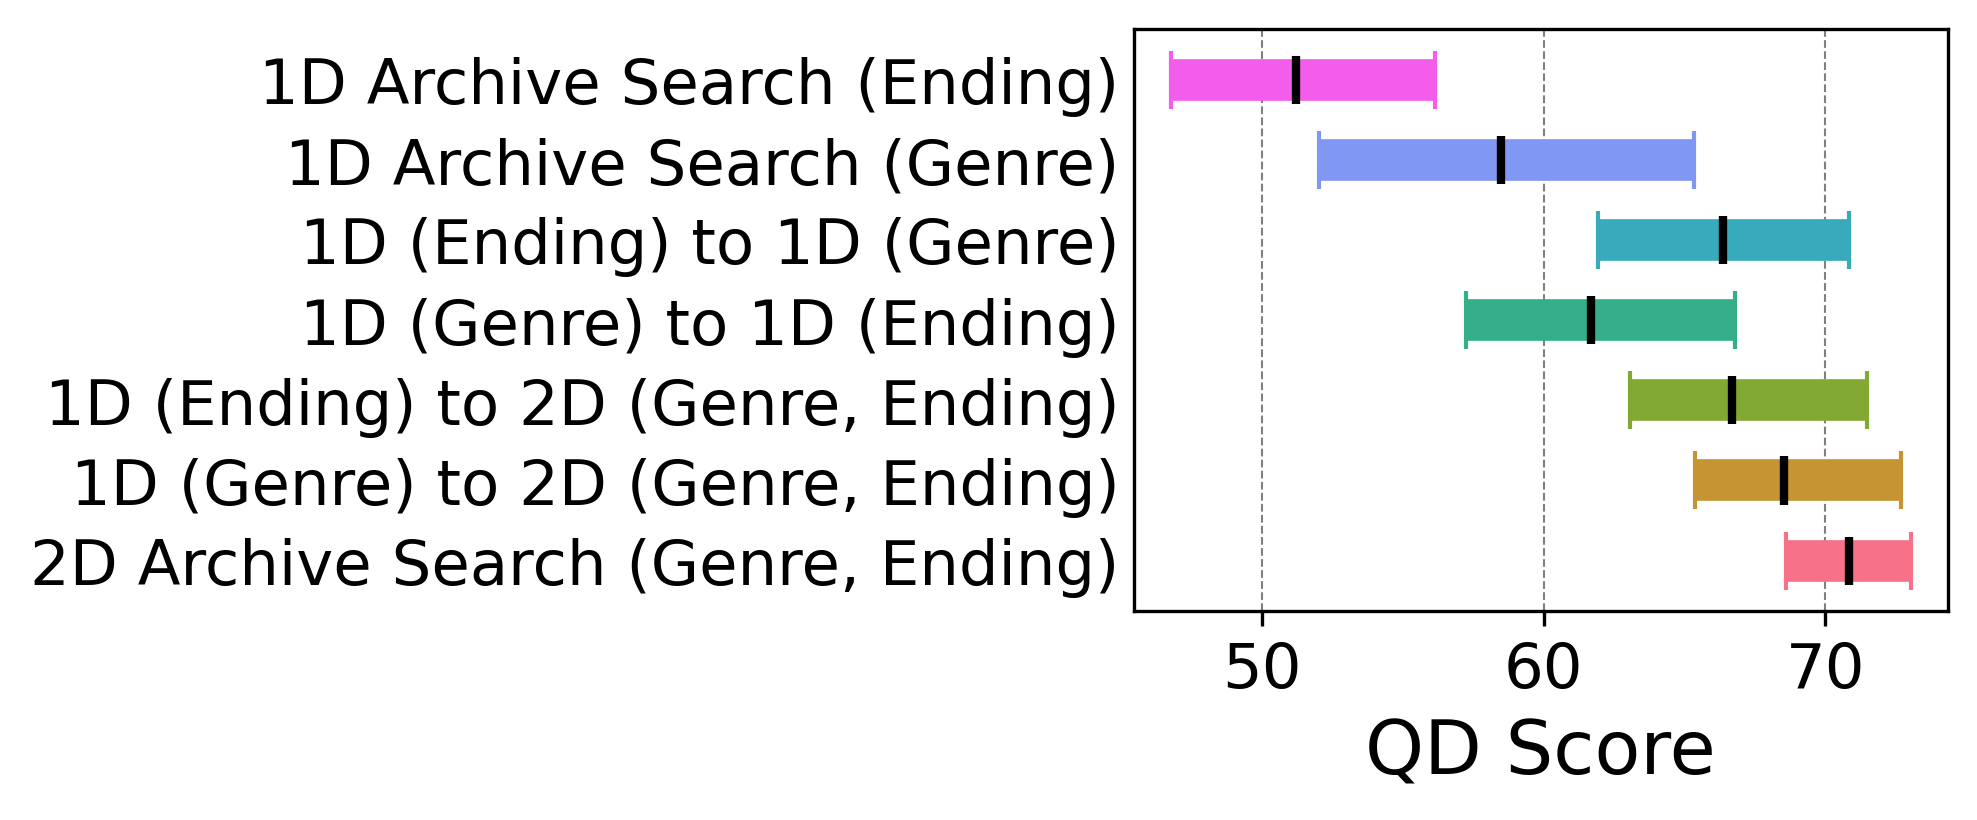
\includegraphics[height=0.105\textheight]{main_figures/extensions/expanding_dims_perf/qd_score.png}
    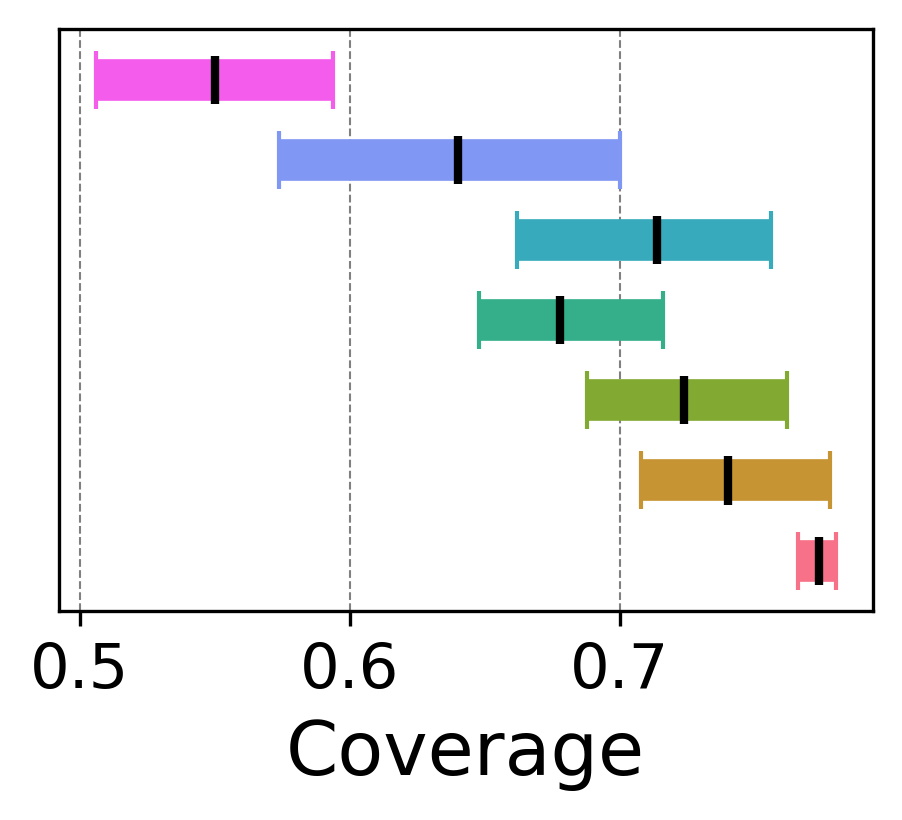
\includegraphics[height=0.105\textheight]{main_figures/extensions/expanding_dims_perf/coverage.png}
    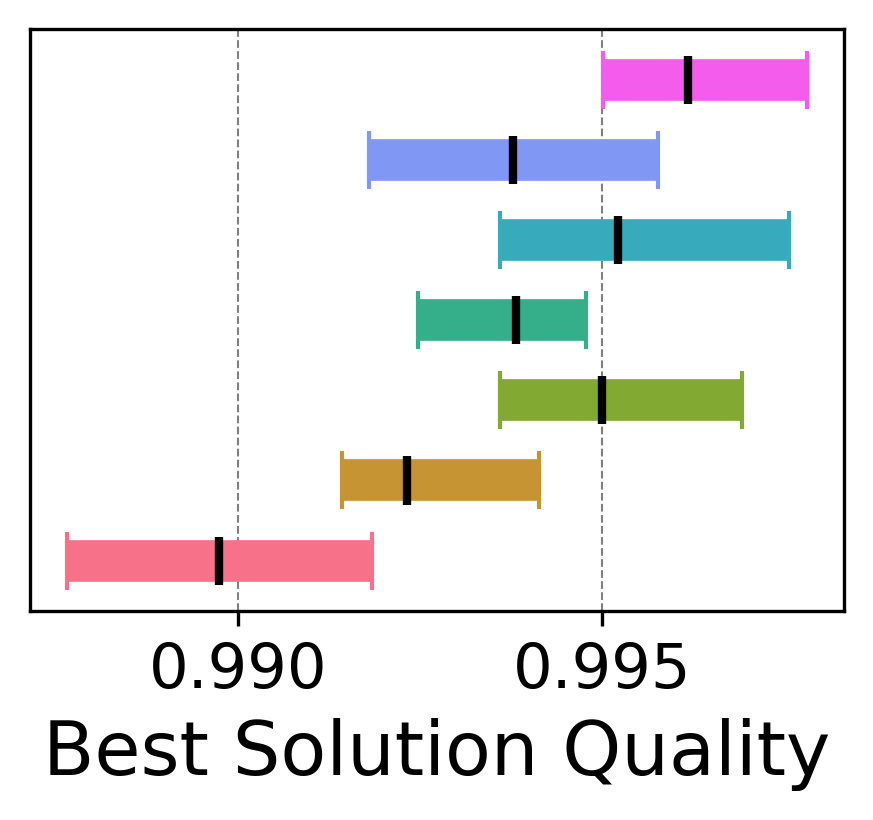
\includegraphics[height=0.105\textheight]{main_figures/extensions/expanding_dims_perf/max_fitness.png}
    \vspace{-0.45cm}
    \caption{\textbf{Expanding (or adapting) archive dimensions for QDAIF during search enables improved search in higher dimensional search spaces compared to searching for solutions along a single 1D diversity axis}. QD score, coverage, and best solution quality stats with mean bootstrapped 95\% CI, across 5 random seed runs. The maximum possible QD score is 100. In both cases of dimension expansion (expanding from 1D (Genre) and 1D (Ending) archives to 2D) enables the performance to approach that of conducting QDAIF search in the full 2D archive, with significant improvement in coverage compared to searching purely in their respective 1D archives. For one case of adaptive archive transition for QDAIF (1D (Ending) to 1D (Genre)), QD score performance and coverage significantly improve compared to searching only in the 1D (Ending) archive.}
    \label{app:fig:perf_expanding_dim}
\end{figure}

\begin{figure}[ht]
    \centering
    % \hspace*{-0.8cm}
    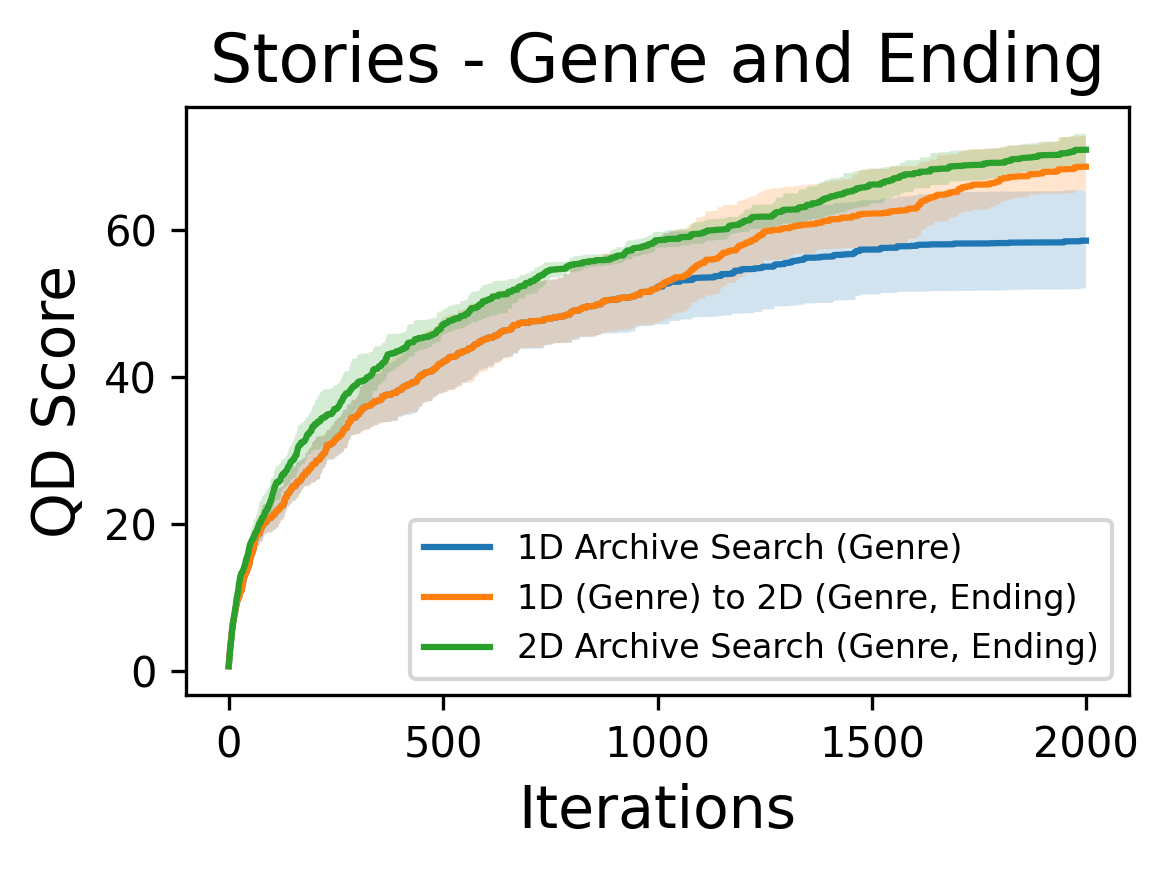
\includegraphics[width=0.49\textwidth]{main_figures/extensions/expanding_dims_plots/qd_score_genre_init.png}
    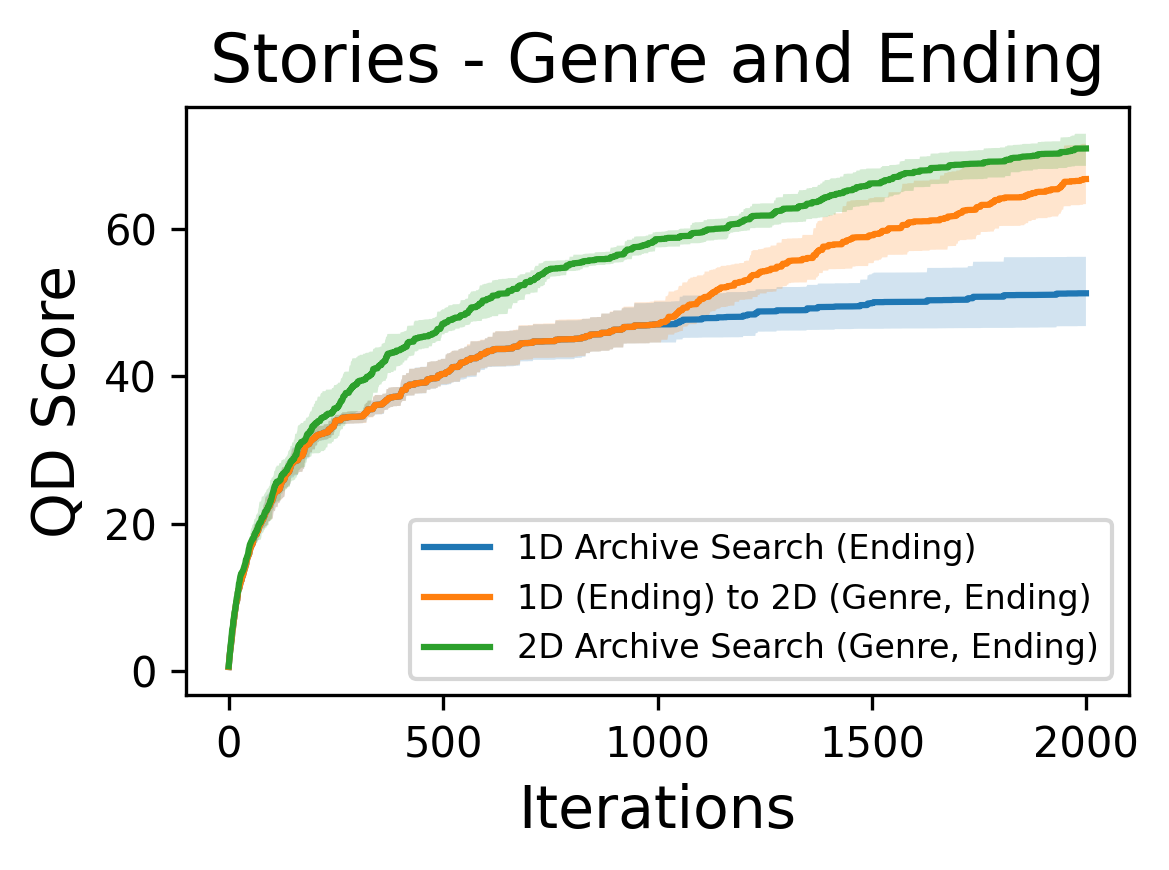
\includegraphics[width=0.49\textwidth]{main_figures/extensions/expanding_dims_plots/qd_score_ending_init.png}
    \vspace{-0.45cm}
    \caption{\textbf{QD score sample efficiency improves from the midway iteration step of orange line plots when the archive dimensions are expanded automatically, in comparison to doing search only in the 1D archive during QDAIF}. Line plots with mean bootstrapped 95\% CI, across 5 random seed runs. The maximum possible QD score is 100. In both cases, either starting with the 1D (Genre) archive (left) or the 1D (Ending) archive (right) and expanding to the 2D archive improves QD score sample efficiency with respect to the 2D archive definition, and approaches performance of the green lines (searching in the 2D archive). The blue lines (1D archive only) converge to a lower QD score during later iterations.}
    \label{app:fig:line_plots_expanding_dim}
\end{figure}

\begin{figure}[ht]
    \centering
    % \hspace*{-0.8cm}
    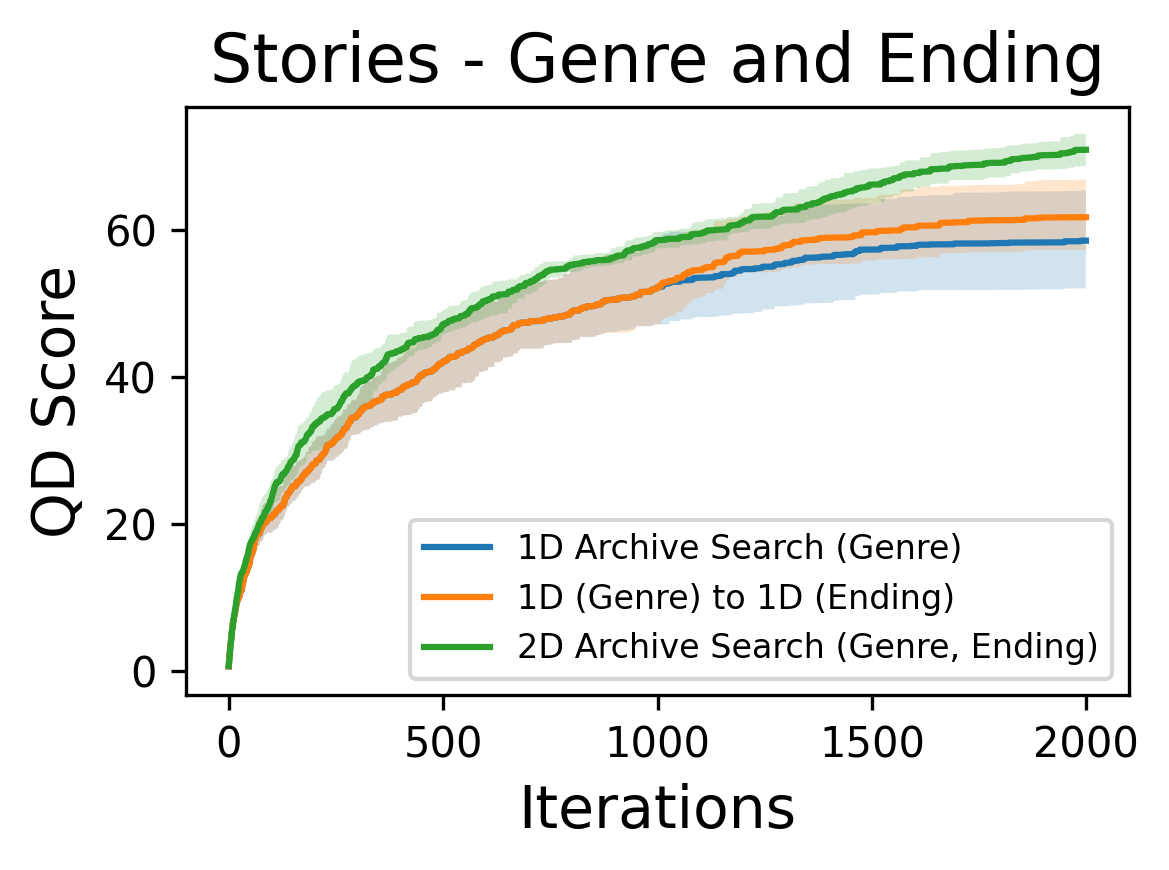
\includegraphics[width=0.49\textwidth]{main_figures/extensions/expanding_dims_plots/qd_score_genre_init_1d_only.png}
    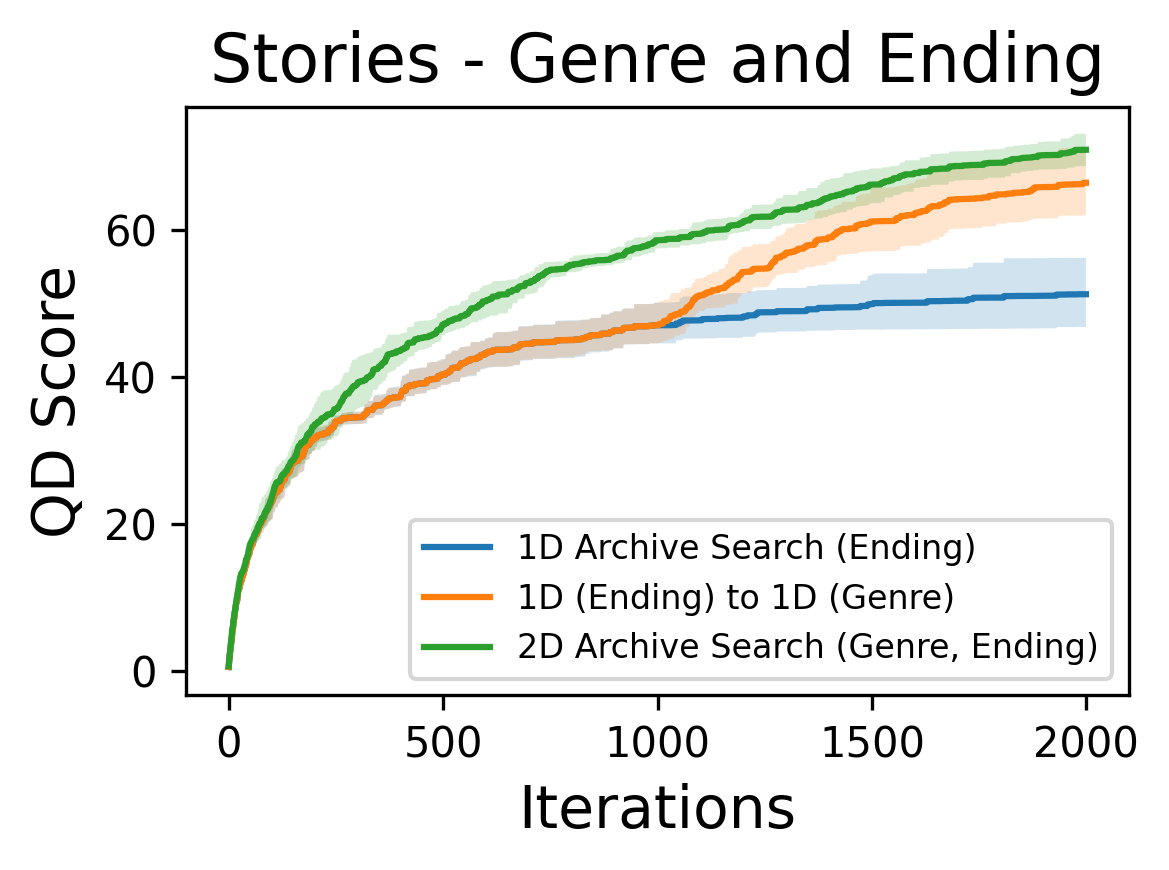
\includegraphics[width=0.49\textwidth]{main_figures/extensions/expanding_dims_plots/qd_score_ending_init_1d_only.png}
    \vspace{-0.45cm}
    \caption{\textbf{QD score sample efficiency improves in one case (right plot) from the midway iteration step of orange line plots when the archive diversity axis is changed to a new diversity measure, but not noticeably improved in another case (left plot), in comparison to doing search without transitioning to a different diversity measure during QDAIF}. Line plots with mean bootstrapped 95\% CI, across 5 random seed runs. The maximum possible QD score is 100. The successful improvement in QD score sample efficiency happens in the case of transitioning from the 1D (Ending) archive to the 1D (Genre) archive, approaching the performance of doing QDAIF in the higher dimensional 2D archive, as shown in the right plot. The case shown in the left plot is still below the performance of QDAIF conducted in the 2D archive, with the orange line converging early to a lower score. The blue lines (1D archive only) converge to a lower QD score during later iterations.}
    \label{app:fig:line_plots_expanding_dim_1d_only}
\end{figure}

\clearpage
\newpage
\subsection{On Finetuning Mutation Models}\label{app:finetune_mutation_discussion}
Prior work on ELM found that using a domain-specific finetuned git diff LM during code generation search led to runs with higher QD score performance compared to when using a pre-trained git diff LM \citep{lehman2022evolution}. The finetuning step relied on a dataset of filtered solutions across several previous runs, adding complexity to the process of creating an effective model for evolving text. To simplify the process, We investigated finetuning on sampled solutions within the same run, during a search that begins with solution generation from a pre-trained LM. We explore the impact of finetuning as a mechanism that can potentially encourage exploitation (through learning to generate higher-quality score solutions) during the search while using evolution to encourage exploration.

To collect samples for finetuning during the search, the first step is collecting a dataset for a given state of the archive, sampling up to 10 solutions with the highest quality score from each bin. Archive bin depth was used to keep track of these finetuning samples (cf. \cref{app:qdaif_lmx}), and introduced in a different application of MAP-Elites for uncertain environments in \citet{flageat2020fast,flageat2023uncertain}. The dataset is shuffled, and then training samples are batched for the LM to finetune on during this phase. Each training sample consists of the prompt that was originally used by a solution to generate an output, and the generated completion text as target tokens for finetuning. We tested both full-model finetuning, and a parameter-efficient finetuning method with sequential adapters finetuning, as described in \citet{he2021towards}. We ran each method using QDAIF LMX(-Near) w/ Seeded-Init (including default method runs without finetuning) on the Stories (Genre and Ending) domain, extending the number of archive dimensions to two. For experiments with adapters, we also conduct runs where the adapter layers are initialized but without doing finetuning, to enable comparisons with adapter finetuning runs accounting for differences in LM architecture introduced by additional layers during the search for runs with finetuning. Still, near-identity initialization (as described in \citet{houlsby2019parameter}) preserves the general performance of the LM.

\paragraph{Finetune-Once.}
This method runs a single finetuning phase during the search before resuming generation with the finetuned LM. We vary two parameters during experiments with Finetune-Once: the iteration step to start the phase (Start), and the number of finetuning steps during this phase (Steps).

\paragraph{Generate-Finetune.}
This method extends Finetune-Once by carrying out the finetuning phase multiple times during the search, repeating the steps of dataset collection and finetuning at regular intervals. We add an additional variable parameter, controlling the regular interval frequency for every set number of generation iterations (Frequency).

\paragraph{Observations.}
We compared the QD score performance between methods across 5 fixed random seed runs. In general, the performance of the Finetune-Once methods with higher scores is comparable to default runs, though slightly lower (but mostly within the confidence interval). For Finetune-Only runs, we observed a potential decrease in performance when using full-model finetuning compared to adapter finetuning, in comparison to conducting these runs without finetuning, with an average $-3.09$ difference in QD score for full-model finetuning compared to $-0.33$ difference for adapter finetuning. It is possible that overfitting on solution examples is more likely for full-model finetuning, which would lead to a decrease in the ability of the LM to evolve new solutions to be accepted in the archive. When we used adapter finetuning as the default for other experiments, we observed a potential decrease in performance and increased variance in performance across multiple seeds when compared to the default method without finetuning. The increase in variance also indicates potential improvements to the search with Finetune-Only in some cases, but further studies are needed on the behavior of search when finetuning on different archive states and constraints to samples collected for finetuning. We can observe a clearer impact of the adverse effects of finetuning from our Generate-Finetune runs. Considering the 95\% confidence interval, the highest mean QD score run we tested from the Generate-Finetune group obtained a performance score of $78.74\pm5.10$ compared to $84.09\pm1.91$ from the default generate-only method. With most runs with Generate-Finetune converging to a lower QD score earlier in the search, it is likely that running standard scheduling the finetuning phase multiple times leads to overfitting of the LM to the point where the model fails to generate new solutions to add to the archive.

\clearpage
\newpage
\subsection{Human Evaluation Study Stats in Writing Domains}\label{app:full_human_eval_tables}
We collected the annotation results from our study, to show the performance of each search method on the tested writing domains, displayed in \cref{app:table_human_eval_baselines_vs_aif}.

\begin{table}[ht]
\caption{\textbf{Extended human eval stats for different creative writing domains, baselines and QDAIF.} The QD score presented here is based on subjective human evaluation results, normalized to a possible range of [1/15, 1]. In terms of the observed difficulty of uncovering the search spaces for each domain from mean quality and QD score stats within each domain, \textbf{Opinions} is the easiest domain (mean QD score is 0.702, mean quality score is 3.613), followed by \textbf{Stories - Ending} (mean QD score is 0.648, mean quality score is 3.575), and \textbf{Stories - Genre} (mean QD score is 0.591, mean quality score is 3.013). The range of metrics between two human evaluators is computed to highlight the variance in some contexts due to more complex aspects of subjectivity in evaluating certain texts.}
\label{app:table_human_eval_baselines_vs_aif}
\vspace{0.2cm}
\centering
\scriptsize
\begin{tabular}{@{}lcccccc@{}}
\toprule
\textbf{Method} &
\makecell[c]{\textbf{Human}\\\textbf{QD score}} & 
\makecell[c]{\textbf{QD score}\\\textbf{range}} &
\makecell[c]{\textbf{Quality}\\\textbf{rating}} &
\makecell[c]{\textbf{Quality}\\\textbf{range}}  & 
\makecell[c]{\textbf{Human-AI}\\\textbf{agreement}} & 
\makecell[c]{\textbf{Human}\\\textbf{agreement}}  \\
\midrule
\multicolumn{7}{c}{Opinions} \\
\midrule
Fixed-Few-Shot & 1.000 & 0.000 & 5.000 & 0.000 & 0.700 & 0.800  \\ 
Shuffling-Few-Shot & 0.728 & 0.056 & 3.600 & 0.800 & 0.700 & 0.800  \\ 
Random-Search & 0.600 & 0.267 & 3.600 & 0.800 & 0.700 & 0.800  \\ 
LMX, Quality-Only & 0.750 & 0.300 & 3.800 & 1.200 & 0.600 & 1.000  \\ 
QDAIF (LMX w/ Zero-Shot Init) & 0.350 & 0.300 & 1.700 & 1.400 & 0.800 & 1.000  \\ 
QDAIF (LMX w/ Seeded Init) & 0.617 & 0.167 & 3.200 & 1.200 & 1.000 & 1.000  \\ 
QDAIF (LMX-Replace w/ Zero-Shot Init) & 0.833 & 0.267 & 4.300 & 1.000 & 0.600 & 0.600  \\ 
QDAIF (LMX-Replace w/ Seeded Init) & 0.739 & 0.078 & 3.700 & 0.600 & 0.700 & 0.800 \\ 
\midrule
\multicolumn{7}{c}{Stories (Genre)} \\
\midrule
Fixed-Few-Shot & 0.650 & 0.167 & 3.400 & 1.600 & 1.000 & 1.000  \\ 
Shuffling-Few-Shot & 0.861 & 0.056 & 4.300 & 0.600 & 0.700 & 0.800  \\ 
Random-Search & 0.683 & 0.100 & 3.400 & 0.800 & 0.700 & 0.400  \\ 
LMX, Quality-Only & 0.600 & 0.267 & 2.900 & 1.400 & 0.700 & 0.800  \\ 
QDAIF (LMX w/ Zero-Shot Init) & 0.200 & 0.000 & 1.400 & 0.400 & 0.400 & 0.600  \\ 
QDAIF (LMX w/ Seeded Init) & 0.767 & 0.133 & 3.700 & 0.600 & 0.800 & 1.000  \\ 
QDAIF (LMX-Replace w/ Zero-Shot Init) & 0.286 & 0.006 & 1.500 & 0.200 & 0.500 & 0.800  \\ 
QDAIF (LMX-Replace w/ Seeded Init) & 0.683 & 0.100 & 3.500 & 0.600 & 0.900 & 0.800 \\ 
\midrule
\multicolumn{7}{c}{Stories (Ending)} \\
\midrule
Fixed-Few-Shot & 0.650 & 0.167 & 4.000 & 0.400 & 0.700 & 0.800  \\ 
Shuffling-Few-Shot & 0.500 & 0.200 & 2.600 & 0.800 & 0.700 & 0.400  \\ 
Random-Search & 0.533 & 0.000 & 2.900 & 1.400 & 0.800 & 0.600  \\ 
LMX, Quality-Only & 0.600 & 0.400 & 3.900 & 0.600 & 0.600 & 0.400  \\ 
QDAIF (LMX w/ Zero-Shot Init) & 0.600 & 0.200 & 3.600 & 0.800 & 0.600 & 0.200  \\ 
QDAIF (LMX w/ Seeded Init) & 0.933 & 0.133 & 4.800 & 0.400 & 0.700 & 0.400  \\ 
QDAIF (LMX-Replace w/ Zero-Shot Init) & 0.500 & 0.333 & 2.600 & 1.600 & 1.000 & 1.000  \\ 
QDAIF (LMX-Replace w/ Seeded Init) & 0.867 & 0.267 & 4.200 & 1.600 & 0.800 & 0.800 \\ 
\bottomrule
\end{tabular}
\end{table}

\clearpage
\newpage
\subsection{On the Differences in Elite Texts across Domains from QDAIF}\label{app:qualitative_summary_qdaif}
We referred to LMX-Near \citep{meyerson2023language} as LMX in the main text for brevity. For more detailed analysis with different mutation operators, we refer to the full name. A summary of human eval stats based on the samples described below can be found in \cref{app:full_human_eval_tables}.

\paragraph{Opinions.}
We report the results from evaluated sets of generated texts from our human study, starting with the Opinions domain in Appendix \crefrange{app:table_eval_opinions_aif_near_seeded}{app:table_eval_opinions_aif_replace_zero} (with qualitative descriptions of the evaluated generated texts in the table captions). Tables are organized in the following order, for each domain: LMX-Near /w Seeded Init (default); LMX-Near /w Zero-Shot Init; LMX-Replace /w Seeded Init; and LMX-Replace /w Zero-Shot Init. Qualitatively, we can see that repetition of phrases appears more often in the samples of generated elite texts from runs using LMX-Near, especially when using Zero-Shot Init. For LMX-Near /w Seeded Init (In \cref{app:table_eval_opinions_aif_near_seeded}), there is frequent repetition of phrases like "I would rather eat scrambled eggs" (third row, bin 9), and "At a restaurant" (fifth row, bin 19). For LMX-Near /w Zero-Shot Init (In \cref{app:table_eval_opinions_aif_near_zero}), there is further repetition of undesired phrases like "Below is a random opinion piece" and "Here is a random opinion piece" in all examples. On the other hand, the generated texts from LMX-Replace (\cref{app:table_eval_opinions_aif_replace_seeded,app:table_eval_opinions_aif_replace_zero} for Seeded Init (default), and Zero-Shot Init methods respectively) lack this output artifact, and received higher quality scores from human feedback overall. Furthermore, texts from LMX-Replace /w Zero-Shot Init received the highest quality score (from humans) compared to the other three methods here, while texts from LMX-Near /w Zero-Shot Init received the lowest quality scores.

\paragraph{Stories - Genre.}
For this domain (with evaluated sets presented in \crefrange{app:table_eval_stories_genre_aif_near_seeded}{app:table_eval_stories_genre_aif_replace_zero}), evaluators found the subjective quality of texts from runs using Seeded Init (default) to be higher than runs using Zero-Shot Init. The stories that were generated with Zero-Shot Init were found to be low in quality due to the presence of attributes such as erroneous titles, and a text style that fails to reflect what's expected in a plausible short story text. Furthermore, the elite stories from the Zero-Shot Init generated sets were more likely to lead to disagreements on the genre between AI feedback and human feedback, with neutral labels given more frequently even for texts in some of the extreme ends of the bins. Given a more open-ended generation task, and a narrow space of desired diversity (focused on the spectrum between two genres), LMX-Near /w Seeded Init (default) (\cref{app:table_eval_stories_genre_aif_near_seeded}) was the most successful method in finding a story for the horror genre niche in Bin 0 (with a low quality score of 2 from evaluators). Other methods either failed to discover a story for this niche, or received an even lower quality score from human feedback.

\paragraph{Stories - Ending.}
For this domain (with evaluated sets presented in \crefrange{app:table_eval_stories_ending_aif_near_seeded}{app:table_eval_stories_ending_aif_replace_zero}), the stories received higher quality scores across sets in comparison to the sets from the \textbf{Stories - Genre} domain, indicating a potentially easier search space when finding stories with different kinds of endings. Still, methods using Seeded Init produced sets of stories that received higher quality scores from evaluators, in comparison to sets from Zero-Shot Init (especially LMX-Replace /w Zero-Shot Init in Table~\ref{app:table_eval_stories_ending_aif_replace_zero}, where the presence of erroneous titles led to lower subjective quality). In spite of the lack of guidance from hand-written prompt examples during initialization, LMX-Near /w Zero-Shot Init (Table~\ref{app:table_eval_stories_ending_aif_near_zero}) managed to produce reasonable stories of above-average quality to cover different ending niches.

\clearpage
\newpage
\subsection{On the Evolution of Generated Texts over Iterations from QDAIF}\label{app:iterations_summary_qdaif}
We describe the evolution of texts from QDAIF with LMX at different search iterations in \crefrange{app:table_iter_opinions_near_zero}{app:table_iter_stories_ending_replace_seed}. One key factor that influences the search is the initialization method - generations in early iterations from Zero-Shot Init methods frequently contain elements that are subjectively different to hand-written examples in the seed texts (in \ref{app:aif_prompts_lmx}). For example, erroneous URLs (in Tables~\ref{app:table_iter_opinions_near_zero},~\ref{app:table_iter_opinions_replace_zero},~\ref{app:table_iter_stories_ending_replace_zero}) and titles (in Tables~\ref{app:table_iter_stories_genre_near_zero},~\ref{app:table_iter_stories_ending_near_zero}) are seen when the possible distribution of outputs is not constrained by seeded in-context examples. This kind of method enables further exploration of output samples, potentially useful in the search of interesting, diverse creative texts. At the same time, more constraints are required from quality assessment using AI feedback in order to control the evolving population of creative texts, towards high-quality, diverse texts. In several cases, outputs from these methods in later iterations show reduced instances of these artifacts compared to early iteration outputs (e.g. in \cref{app:table_iter_stories_ending_replace_zero}), but can be missed when AI feedback evaluation at times is misaligned with human preferences (e.g. in \cref{app:table_iter_stories_genre_near_zero}). Still, using Seeded Init does not guarantee enough guidance to completely remove undesired features from generations in later iterations. For example, texts with repetitive phrases can be seen during later iterations on the Opinions domain from methods using Seeded Init (see \cref{app:table_iter_opinions_near_seed,app:table_iter_opinions_replace_seed}. In general, Seeded Init runs are more likely to lead to high-quality texts across niches, in comparison to Zero-Shot Init runs, especially according to human evaluation (see Table \ref{table:mean_human_eval_baselines_vs_aif}), especially for more challenging, open-ended domains such as story-writing. Furthermore, a side-effect of the increased likelihood of subjective reward hacking when using Zero-Shot Init for runs. Still, QDAIF can still work well with Zero-Shot Init, especially in combination with LMX-Replace, as shown in the results from the Opinions domain experiments.

\subsection{On the Differences in Elite Texts across Domains from Baseline Methods}\label{app:qualitative_summary_baseline}

Evaluated sets are presented in \crefrange{app:table_eval_opinions_b1}{app:table_eval_opinions_b4}, \crefrange{app:table_eval_stories_genre_b1}{app:table_eval_stories_genre_b4}, and \crefrange{app:table_eval_stories_ending_b1}{app:table_eval_stories_ending_b4} for Opinions, Stories - Genre, and Stories - Ending domains respectively. \baseone{} and \basetwo{} consistently adhere to the style and structure of the seeded examples. \basethree{} exhibits more variability, with discrepancies in feedback between humans and AI most evident in the Opinions domains and challenges in story consistency and character inclusion. \basefour{} further highlights these discrepancies, especially where repetitive or contradictory opinions are concerned. Across narratives, \basefour{} tends to miss character details or produce underdeveloped storylines, despite sometimes receiving high AI feedback. A recurring theme across all baselines is the differential perception of quality between human and AI feedback, with repetitive narratives, character relevance, and development being central points of contention.

\subsection{On the Evolution of Generated Texts over Iterations from Baseline Methods}\label{app:iterations_summary_baseline}
Qualitatively, both \baseone{} and \basetwo{} consistently replicate concepts and expressions from the few-shot examples, at times directly copying entire segments (Tables~\ref{tab:b1-qualitative-opinion}, \ref{tab:b1-qualitative-story}, \ref{tab:b2-qualitative-opinion}, and \ref{tab:b2-qualitative-story}). This suggests a potential over-reliance on the few-shot examples, hindering the generation of diverse solutions. In contrast, \basethree{} aims to foster diversity by retaining all entries into the pool. However, this approach may unintentionally impede optimization for higher fitness solutions. Notably, fitness values of generated entries using \basethree{} in later iterations persistently fall short (Tables~\ref{tab:b3-qualitative-opinion} and \ref{tab:b3-qualitative-story}). The crux of this issue seems to arise from the strategy's indiscriminate inclusion of entries, even those with low fitness. Consequently, when these low-fitness examples are integrated into few-shot prompts, they influence the generation of subsequent entries, often resulting in similarly suboptimal outcomes. Lastly, \basefour{} introduces a fitness-centric approach, retaining only those solutions with the highest fitness. While entries from its early iterations display a diverse range of phenotype and fitness values, later iterations, with a noticeable uptick in fitness scores, tend to use similar phrases and writing styles (Tables~\ref{tab:b4-qualitative-opinion} and \ref{tab:b4-qualitative-story}). This suggests that stringently prioritizing high-fitness solutions may prevent the exploration of more varied or potentially better solutions.

\clearpage
\newpage
\subsection{On the Use of Different Versions and Types of Models for Poetry}\label{app:discuss_gpt4_methods}
We show QD score line plots comparing QDAIF against other methods in \cref{app:fig:qdaif_rewrite_poetry_line_plot}. We noted that in addition to improvement in QD score from QDAIF, CI gaps from experiments using GPT-4 were qualitatively wider as shown in the line plots. This suggests the potential of using different models for prompted variation of solutions in creative domains, with the possibility that certain models are more capable of generating slightly more diverse solutions (that may better cover the space of possible solutions) (cf. \cref{app:discuss_poetry_qdaif_evolution} on differences in rewriting behavior from different models). Although QDAIF significantly improves on relevant non-QD methods through the evolution of solutions via rewriting, the challenge remains in uncovering all possible solutions in the diversity space of interest (e.g. empty bins in experiment archive, or categories that can further differentiate subjectively unique solutions); it is difficult for existing models without explicit guidance on the desired poem categories to know that these exist in the space of possibilities, in a similar sense that the average person may not know what's the most distinct variation that can be applied to rewriting poems (from the wide space of possible poetry). This issue manifests even in simple domains such as random number generation \citep{llm_sampling_renda_hopkins_2023}. Coverage is possible with methods that guide LMs on the desired (cf. \cref{app:fig:qdaif_guided_poetry_line_plot}), with the added benefits of grounding on poems of interest through seed parent poems (cf. \cref{app:discuss_poetry_qdaif_evolution}), but future work is needed to create systems that can successfully navigate in solution exploration beyond what is currently known or defined (i.e. through limited genre and tone categories) during a search at hand \citep{zhang2023omni}, perhaps even through the discovery of new types of poems, unlike ones that have been written by human poets.

\cref{app:fig:poetry_gen_model_used} compares the performance of different models used for generation and rewriting with each search method. We found higher CI gaps from runs using GPT-4 with \poembaseone{}, \poemablation{}, and QDAIF (LMX-rewrite), in comparison to GPT-3.5-Turbo. The difference in rewriting behavior between GPT-4 and GPT-3.5-Turbo may contribute to variation in performance predictability during QDAIF (cf. \cref{app:discuss_poetry_qdaif_evolution}). Additionally, GPT-4 more often gives higher QD score performance in some cases (\poembaseone), while GPT-3.5-Turbo can improve sample efficiency during search in other cases (\poemablation, \poembasetwo). Interestingly, improvements in sample efficiency from GPT-3.5-Turbo may not translate fully to support interesting discovery of new solutions in poetry during QDAIF (cf. \cref{fig:poem_evolution_gpt_3_5}). Results further highlight the need to investigate the potential of different models for solution variation in QDAIF.

We noted from runs in the Poetry domain using an older version of GPT-4 (April 2023) for the experiments that QDAIF saw potential improvement in performance compared to baseline methods. There is a risk of variation in performance and search behavior due to the nature of changing model versions; the impact would be on the generation, re-writing, and evaluation of poems. We observed in \cref{app:fig_old_version_poetry_results} that QDAIF successfully populates the archive with high-quality poems, leaving only three bins empty. In contrast, \poembaseone{} (Baseline) only fills the archive sparsely, demonstrating that asking for creative output from a single LM prompt often results in a lack of diversity. Furthermore, more bins remain empty in the archive generated by \poembasetwo{} (Targeted Baseline). Overall, QDAIF achieved higher QD scores in experiments with older models and covers more bins in the archive than \poembaseone{} and \poembasetwo{} as can be seen \cref{app:fig_old_version_poetry_results}. This hints at another potential benefit of QDAIF with \qdaifguided, where a combination of instructed guidance and evolution could also lead in improvements to QD score with some models.

\begin{figure}[ht]
    \centering
    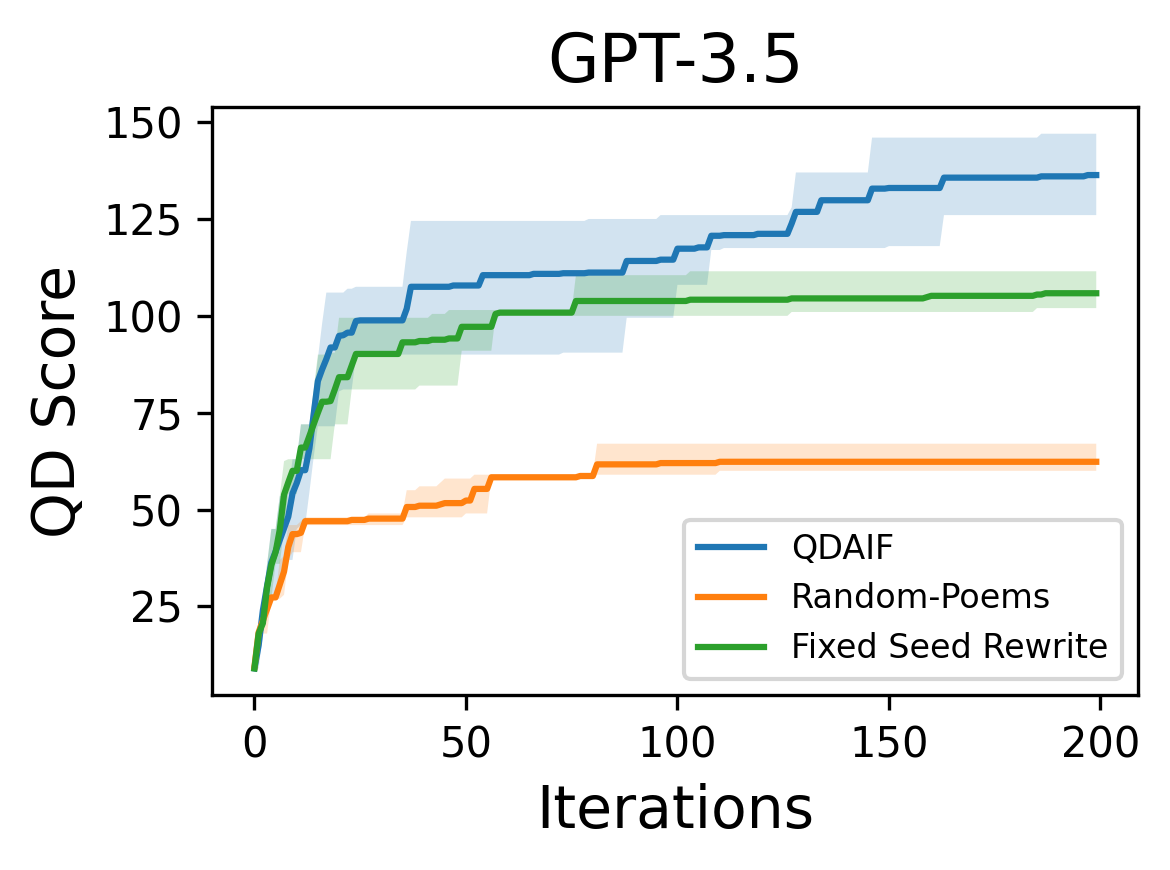
\includegraphics[width=0.49\textwidth]{main_figures/poetry/updated_runs/comparison/gpt_35_rewrite.png}
    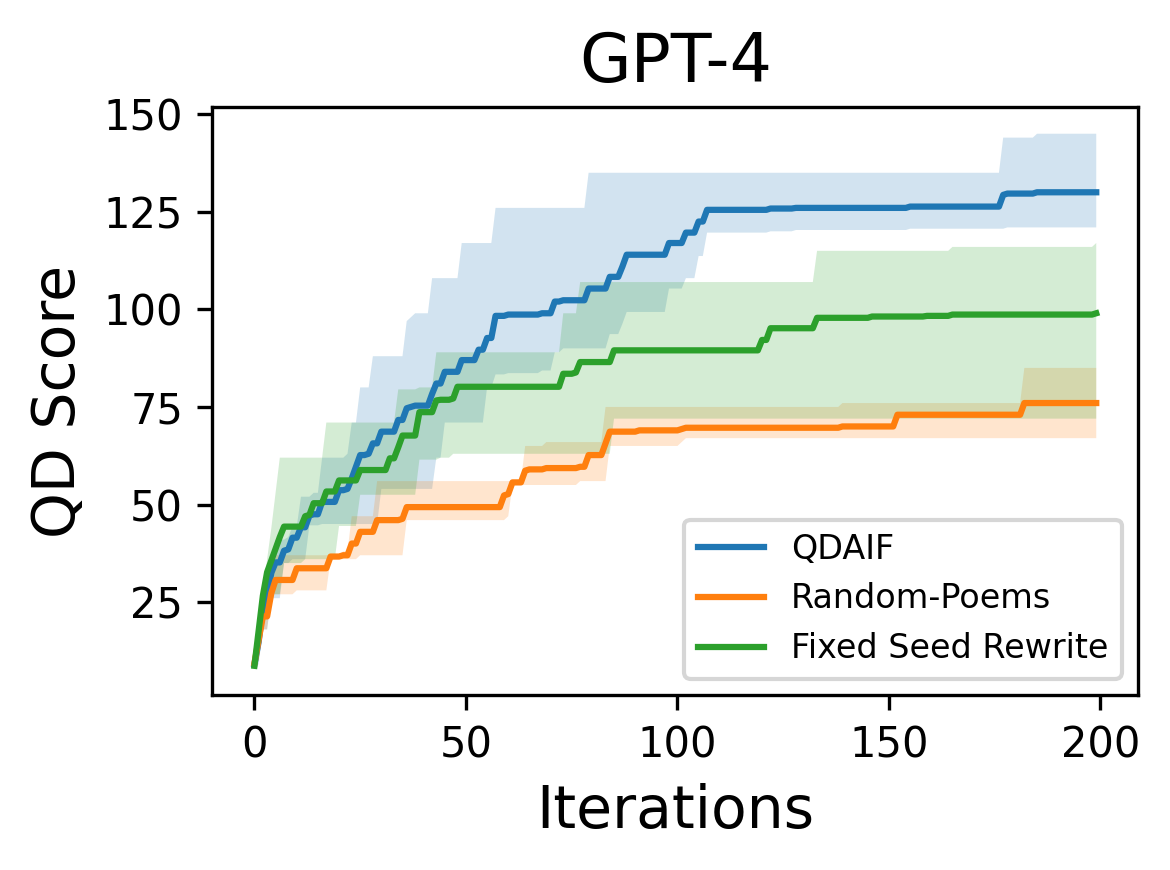
\includegraphics[width=0.49\textwidth]{main_figures/poetry/updated_runs/comparison/gpt_4_rewrite.png}
    \caption{\textbf{QDAIF (\qdaifrewrite) outperforms the baseline, \poembaseone, and an ablation, \poemablation, in terms of QD score, across all generation models tested.} 95\% CI of mean is shown for stats across 3 random reruns. We observed from the Mann-Whitney U Test that QDAIF achieves greater QD score than other methods ($p \leq 0.05$). The step of rewriting a poem (\poemablation) is shown to improve QD score more often than simply requesting poems (\poembaseone), while the additional step of evolutionary search (QDAIF) enables additional improvement. With GPT-3.5(-Turbo), non-QDAIF methods tend to have narrower CIs, indicating higher predictability of reduced performance.}
    \label{app:fig:qdaif_rewrite_poetry_line_plot}
\end{figure}

\begin{figure}[ht]
    \centering
    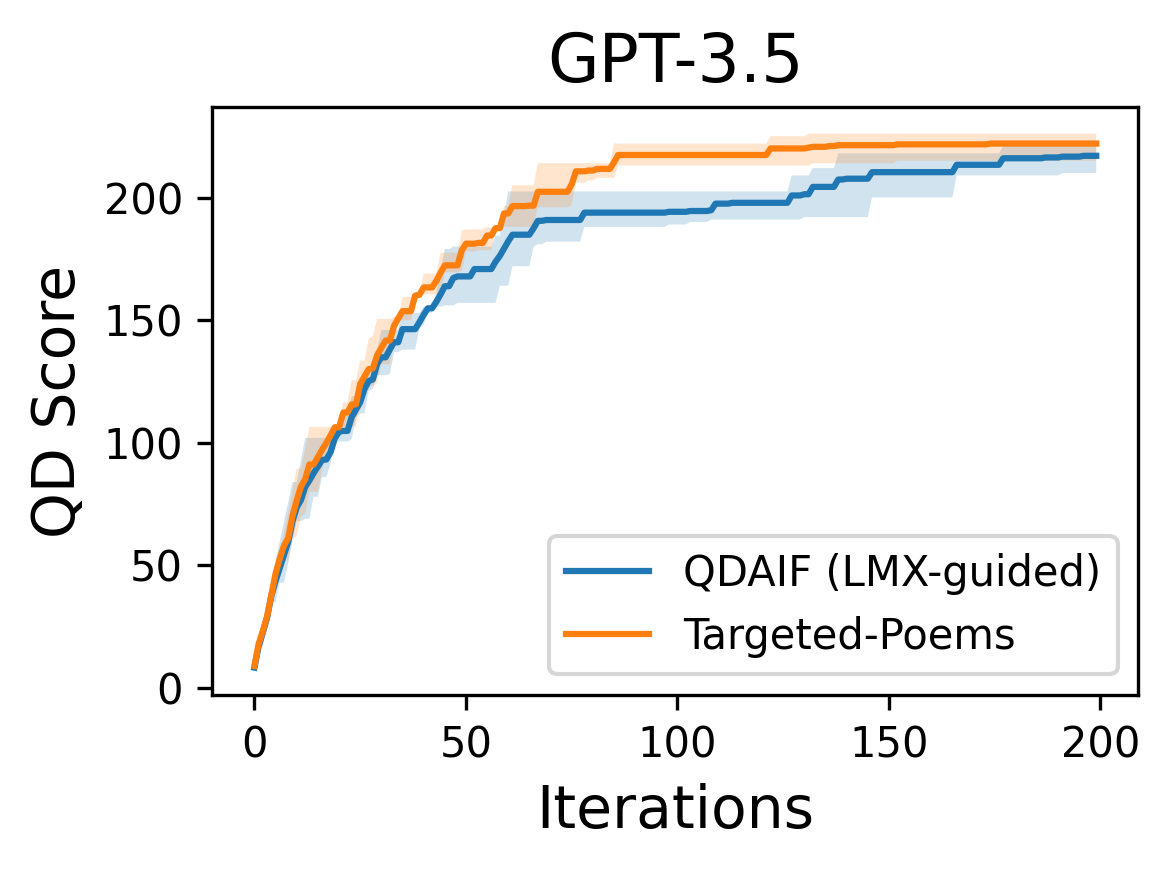
\includegraphics[width=0.49\textwidth]{main_figures/poetry/updated_runs/comparison/gpt_35_guided.png}
    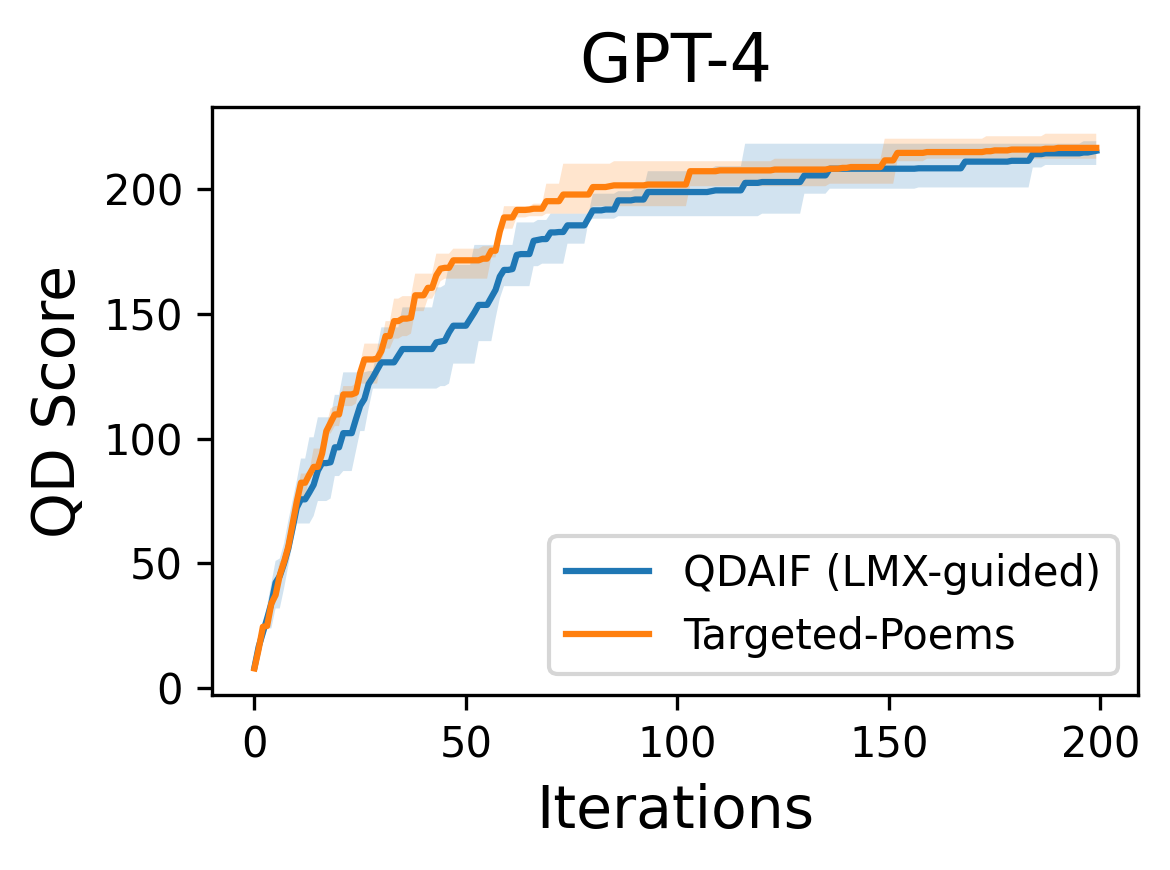
\includegraphics[width=0.49\textwidth]{main_figures/poetry/updated_runs/comparison/gpt_4_guided.png}
    \caption{\textbf{QDAIF (\qdaifguided) is on par with \poembasetwo, while preserving the benefits of diverse evolution of poems stemming from a seed poem (cf. \cref{app:discuss_poetry_qdaif_evolution}).} 95\% CI of mean is shown for stats across 3 random reruns. All methods incorporate guidance on the desired genres and tones in poems during search, and models used are capable of covering all the designated archive bins with relevant diverse, high-quality poems. All methods can quite easily cover the 25 bins of the archive within the number of iterations.}
    \label{app:fig:qdaif_guided_poetry_line_plot}
\end{figure}

\begin{figure}[ht]
    \centering
    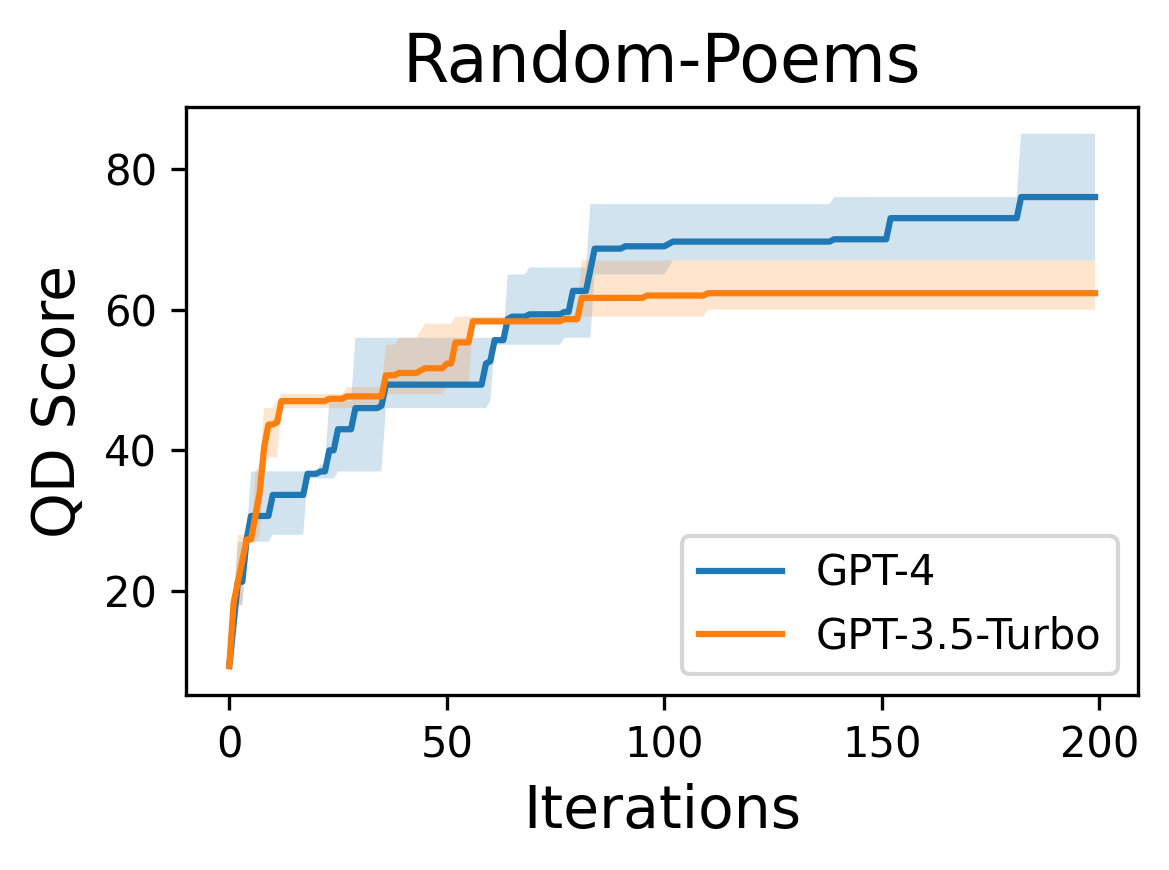
\includegraphics[width=0.49\textwidth]{main_figures/poetry/updated_runs/gen_model_compare/random_poems.png}
    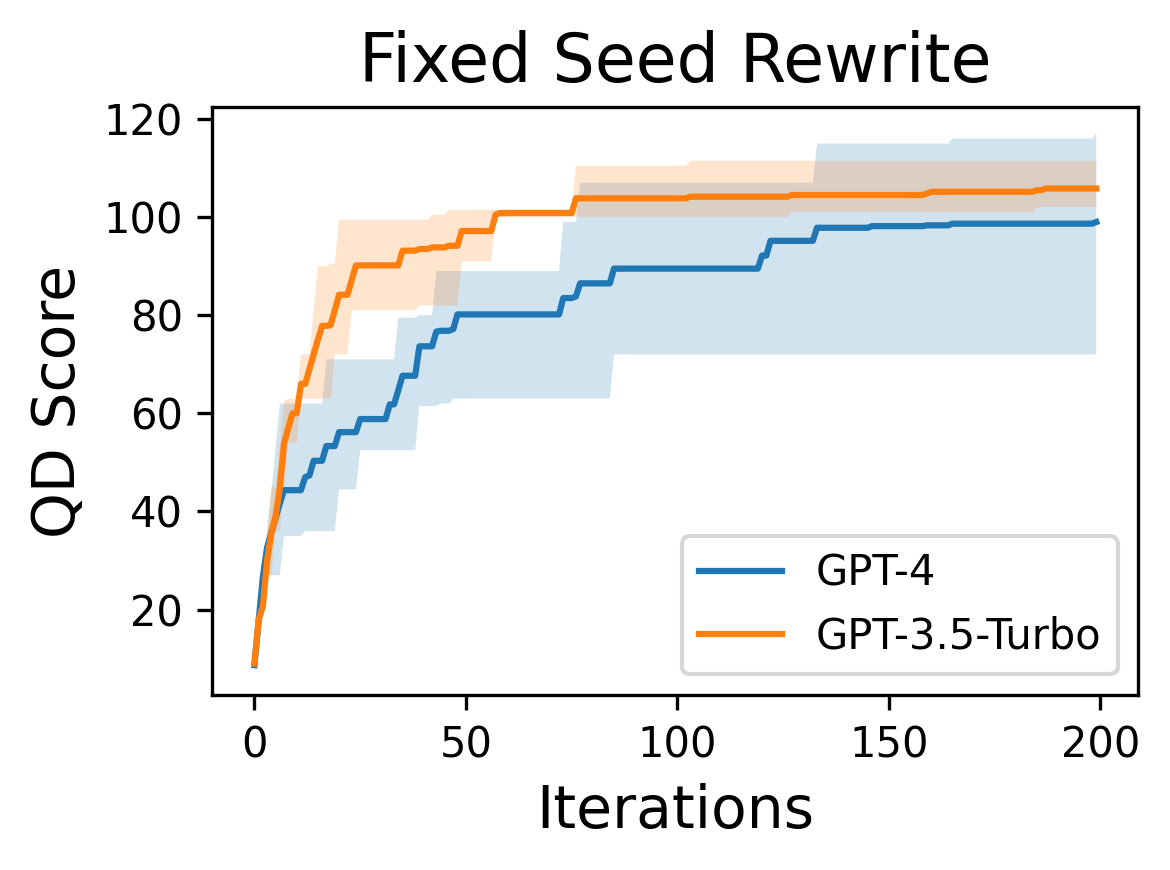
\includegraphics[width=0.49\textwidth]{main_figures/poetry/updated_runs/gen_model_compare/fixed_rewrite.png}
    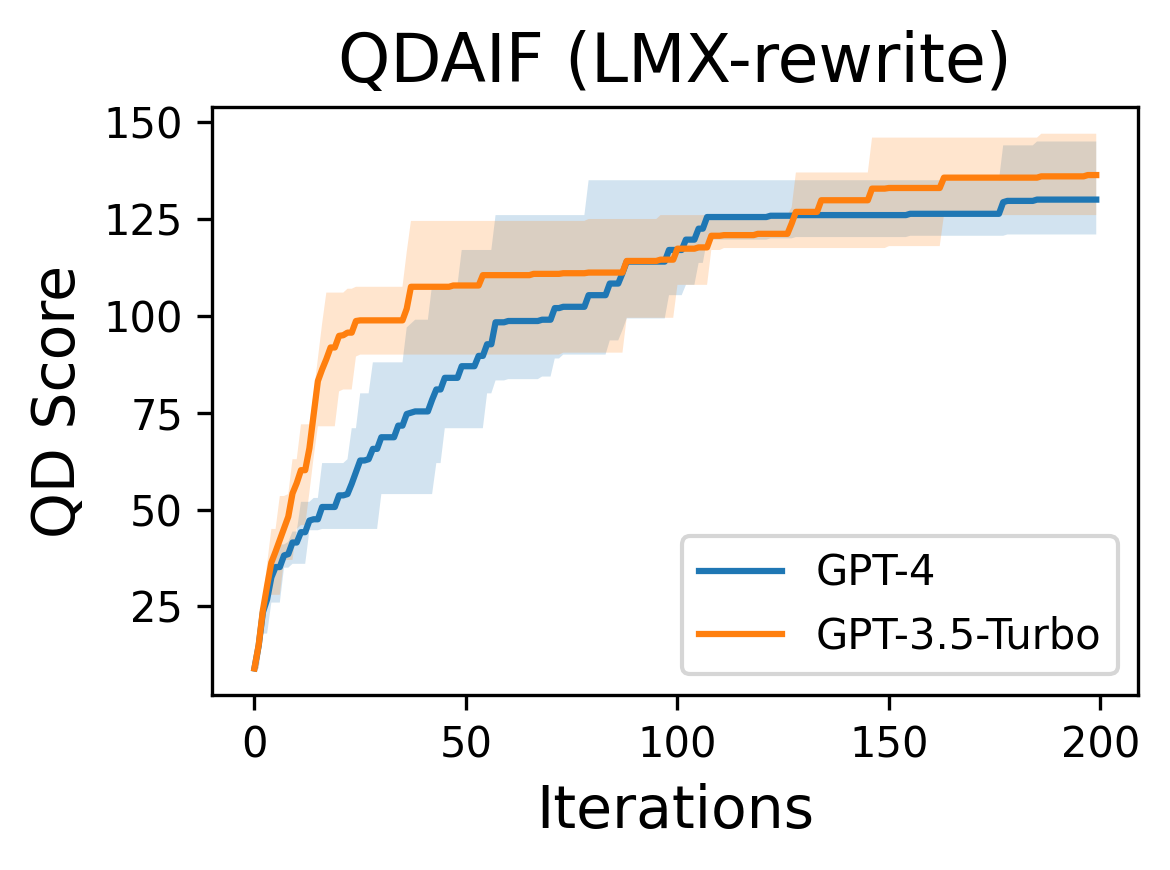
\includegraphics[width=0.49\textwidth]{main_figures/poetry/updated_runs/gen_model_compare/qdaif.png}
    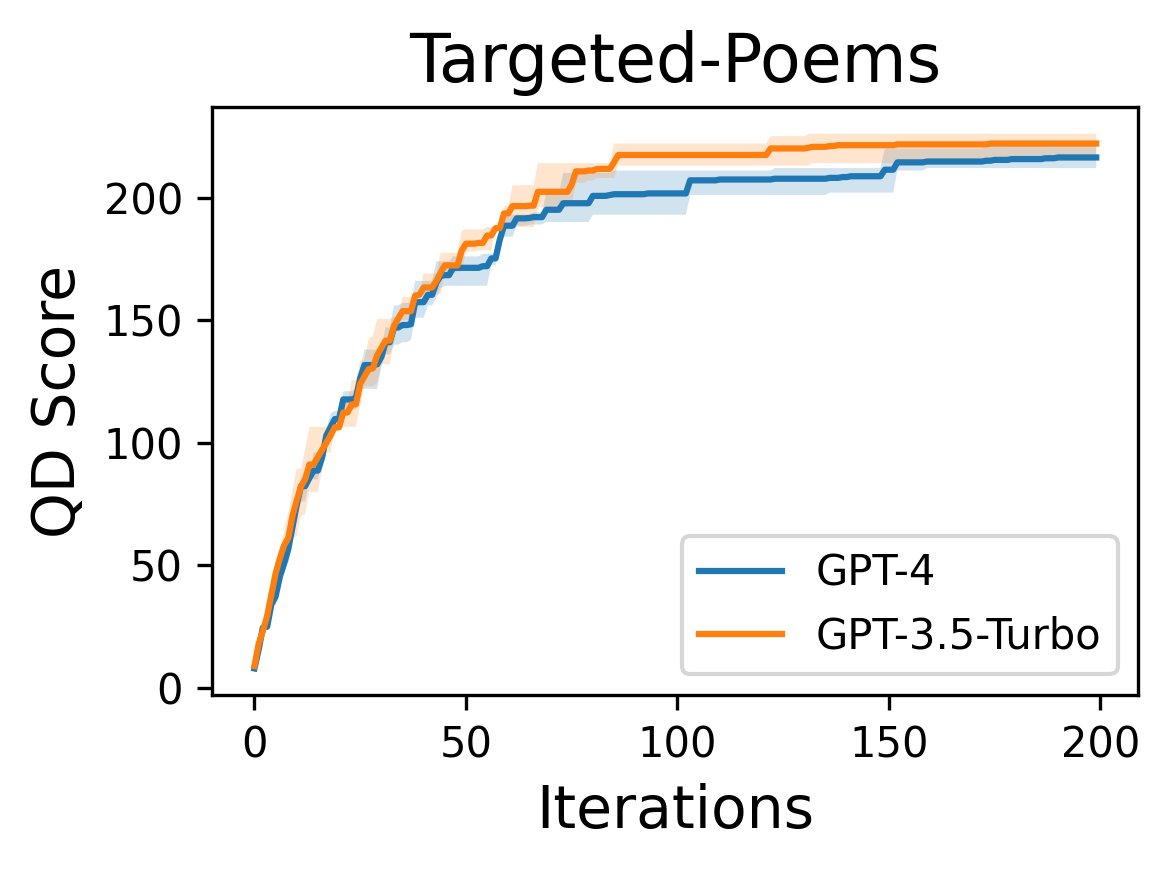
\includegraphics[width=0.49\textwidth]{main_figures/poetry/updated_runs/gen_model_compare/targeted_poems.png}
    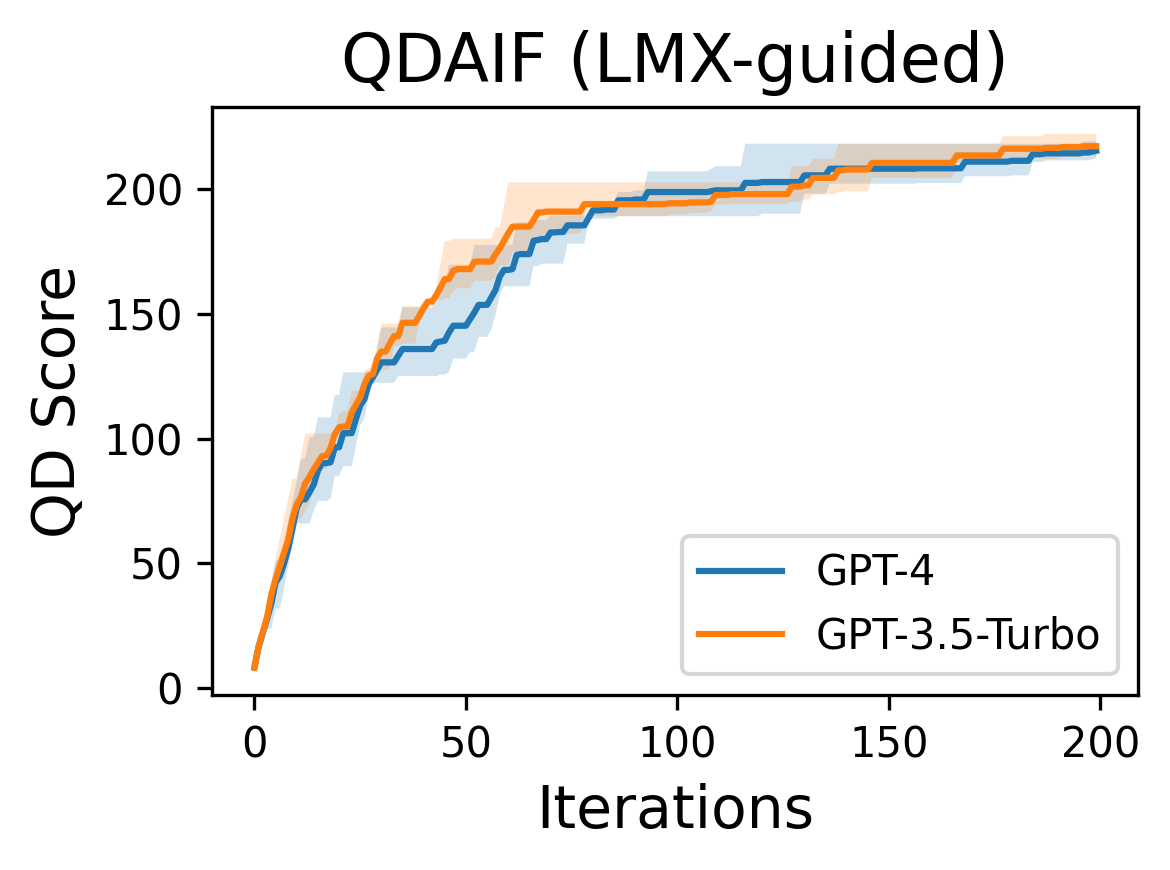
\includegraphics[width=0.49\textwidth]{main_figures/poetry/updated_runs/gen_model_compare/qdaif_guided.png}
    \caption{QD score performance (with 95\% CI from 3 random reruns) for each method varying the model used for generation/rewriting. The evaluation model is GPT-4 \citep{openai2023gpt4} for all runs here. In some cases, GPT-4 more often achieves a higher score (e.g. with \poembaseone), while in other cases, GPT-3.5-Turbo achieves improved sample efficiency over iterations of search (e.g. with \poemablation, \poembasetwo). Wider CIs in some runs with GPT-4 indicate higher unpredictability in performance, and potentially a wider scope in possible outputs that may or may not lead to higher score.}
    \label{app:fig:poetry_gen_model_used}
\end{figure}

\begin{figure}[ht]
    \centering
    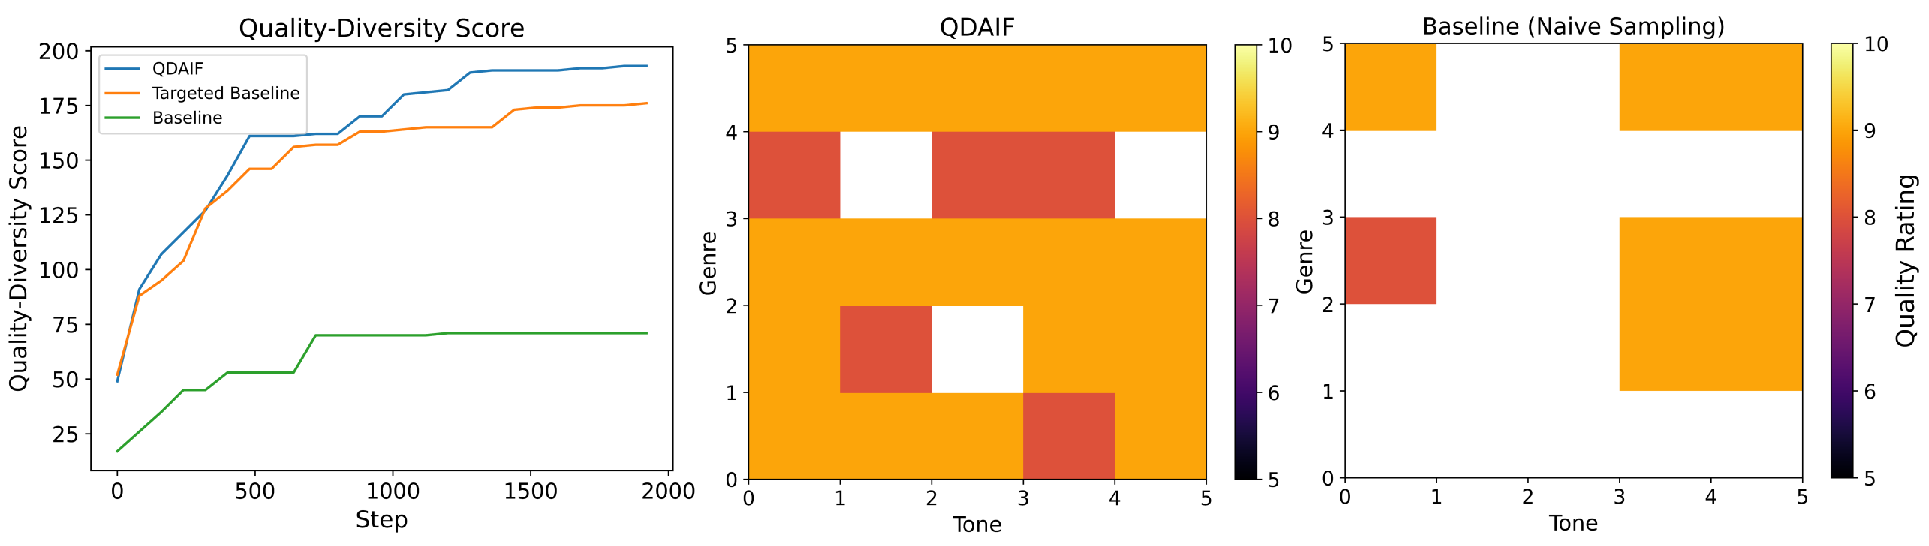
\includegraphics[width=\textwidth]{main_figures/poetry/QDAIF_Poetry_Horizontal.pdf}
    \caption{\textbf{QDAIF (blue, middle) covers more the space of diverse poetry with high-quality solutions compared to baselines.} When compared against a targeted mutation baseline (\poembasetwo, orange), QDAIF attains higher QD scores throughout evolution, and covers a significantly larger portion of the search space than a fully random baseline (\poembaseone{}, green, right). This is for runs with an older version of GPT-4.}
    \label{app:fig_old_version_poetry_results}
\end{figure}

\clearpage
\newpage

\subsection{On the Evolution of Poems through Inspired Rewriting}\label{app:discuss_poetry_qdaif_evolution}
Instead of generating poems completely from scratch, users may generally prefer to have models re-write their draft poems. \cref{fig:poem_evolution_gpt_4} shows an example of the capabilities of GPT-4 using \qdaifguided{}, by starting off from the seed poem and continuing a chain of evolution in high-quality poems across different genres and tones. The evolving poetry chain shown in the figure is the longest continuous one discovered during the search, where the most repeated rewrites occurred starting from the seed poem. Rewrites with the model qualitatively gave meaningful variations in poems that transfer connective imagery with twists in rhythm and connotations, depending on the target genres and tones. At the same time, We found that even when GPT-4 is specifically prompted to craft a poem of a particular genre and tone, subsequent evaluation using the same LM does not always deem it as having the same targeted genre or tone. This underscores a widely recognized gap between text generation and discrimination \citep[Page~12]{saunders2022self}. This is clear from several of the poems classified as hymns, but containing multiple 5-line verses similar to the style of a limerick (while not generating a typical single-verse limerick). It was likely references to religious imagery in later verses, as well as the multi-verse structure that influenced the evaluation for the closest genre.

\cref{fig:poem_evolution_gpt_3_5} shows another example of a chain from using GPT-3.5-Turbo. We found qualitatively that using GPT-4 led to more interesting variations of new poems during rewriting in comparison to GPT-3.5-Turbo rewrites. This is more clear from the repetition of "In fields of emerald, a gentle sway" at the start of each poem following the mysterious sonnet. 

Future research is needed to study the behavior of chained rewriting over stepping stones with current foundation models \citep{nguyen2015innovation,nguyen2016understanding}. \citet{secretan2011picbreeder} found that from user studies in Picbreeder, a tool for evolving images through human-in-the-loop, accumulating divergent chains of solutions of growing complexity from different users (carrying out the evolution of diverse images) is important for a search that is focused on discovering meaningfully interesting and diverse artifacts. \citet{gaier2019quality} validated the potential of QD approaches in enabling the discovery of intermediate solutions that overcome the challenge of escaping undesired local minima (missing promising trajectories to desired solutions) faced by objective-based search \citep{stanley2015greatness}. By leveraging goal-switching \citep{mouret2015illuminating}, QD search was able to maintain enough diversity in the population to enable the discovery of solutions that appear more like targets of interest, significantly outperforming a single objective optimization approach (which generated solutions that resembled primitive patterns unlike the targets) \citep[Chapter~4]{gaier2020accelerating}. This property of QD search is especially important in solution spaces where even slight perturbations in solutions can lead to significant (and often unexpected) qualitative changes in solution properties. This can apply to representations from Compositional Pattern Producing Networks (CPPNs) \citep{stanley2007compositional}, and text representations themselves, where minor changes to certain parts of text can lead to significant changes in passage tone, imagery, or even functionality of code \citep{lehman2022evolution}. Properties of chained divergence as demonstrated in the Poetry domain could inspire further directions in designing new systems with QDAIF.

\begin{figure}[ht]
    \centering
    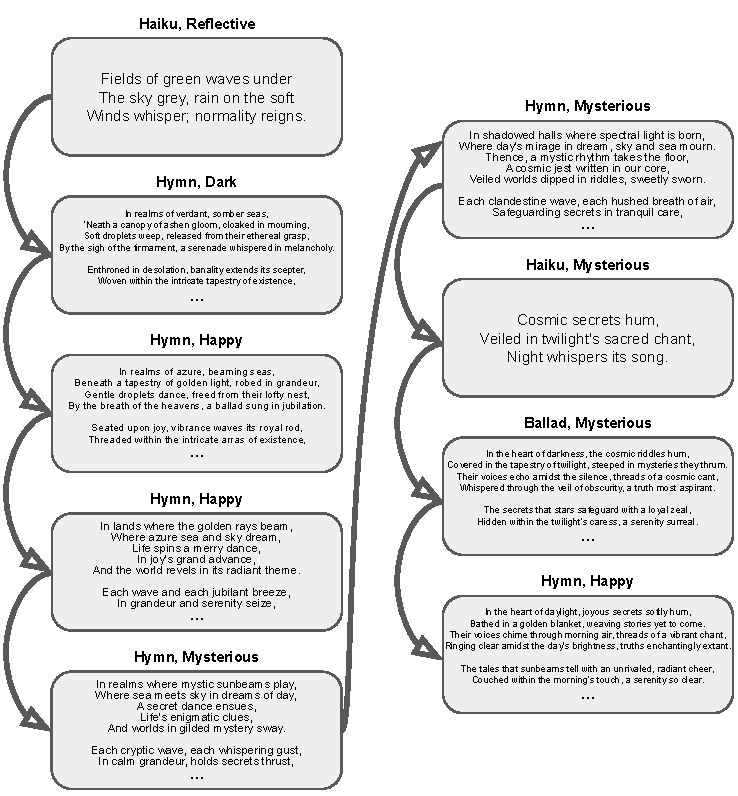
\includegraphics[width=\textwidth]{main_figures/poetry/updated_runs/poem_mutations_gpt_4.pdf}
    \caption{\textbf{QDAIF is enabled by guided poem rewriting. With GPT-4 \citep{openai2023gpt4}.} Starting with a reflective haiku seed poem, the reference to "fields of green waves" and "sky grey, rain" inspires the next dark hymn poem with "verdant, somber seas" and "canopy of ashen gloom", followed by further chains of inspired rewriting. The imagery and choice of words evolve with varying outputs as poems of different genres and tones are generated. We noted that not all poems had evaluated genres and tones that matched their target ones during prompted rewriting, for example, with the hymns with multiple 5-line verses being a result of limericks as the target.}
    \label{fig:poem_evolution_gpt_4}
\end{figure}

\begin{figure}[ht]
    \centering
    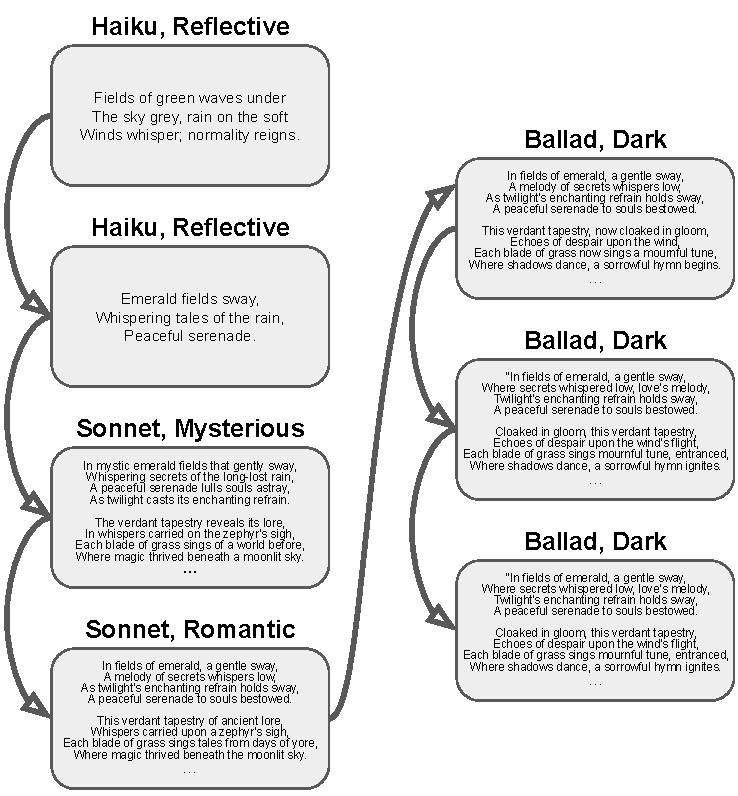
\includegraphics[width=\textwidth]{main_figures/poetry/updated_runs/poem_mutations_gpt_3_5.pdf}
    \caption{\textbf{QDAIF is enabled by guided poem rewriting. With GPT-3.5-Turbo.} The evolved poems cover different genres and tones following inspiration from the seed poem. However, there is repetition of "In fields of emerald, a gentle sway" at the start of each poem following the mysterious sonnet. GPT-4 improves on the ability to rewrite, suggesting that more capable models are also able to give more interesting variations to creative texts.}
    \label{fig:poem_evolution_gpt_3_5}
\end{figure}

\clearpage
\newpage

\subsection{Examples from the Poetry Domain}\label{app:overview_poetry_examples}

Figures~\ref{fig:poem_examples0}, \ref{fig:poem_examples1}, and \ref{fig:poem_examples2} show some generated poems of different quality, genres, and tones. Noticeably, hymns, limericks, ballads, and sonnets that are rates as higher quality tend to be longer, and more closely align with the defining characteristics of their respective genres. For example, the hymn evaluated at 9/10 quality has phrases like "celestial delight", "under heaven's vault", and "seek divine in the ordinary's course", showcasing a worshipper's perspective towards divinity, a trait more pronounced than in an 8/10 rated hymn (Figure~\ref{fig:poem_examples0}). The sonnet with a 9/10 quality rating demonstrates a more consistent rhyme scheme, where all the end words in the same quatrain rhyme, compared to the one rated as 7/10 quality (Figure~\ref{fig:poem_examples2}).

\begin{figure}[ht]
    \centering
    \includegraphics[width=\textwidth]{images/example_poetry0.pdf}
    \caption{Examples of different quality mysterious hymns and reflective limericks generated and evaluated using GPT-4.}
    \label{fig:poem_examples0}
\end{figure}
\begin{figure}[ht]
    \centering
    \includegraphics[width=\textwidth]{images/example_poetry1.pdf}
    \caption{Examples of different quality happy ballads and dark haikus generated and evaluated using GPT-4.}
    \label{fig:poem_examples1}
\end{figure}
\begin{figure}[ht]
    \centering
    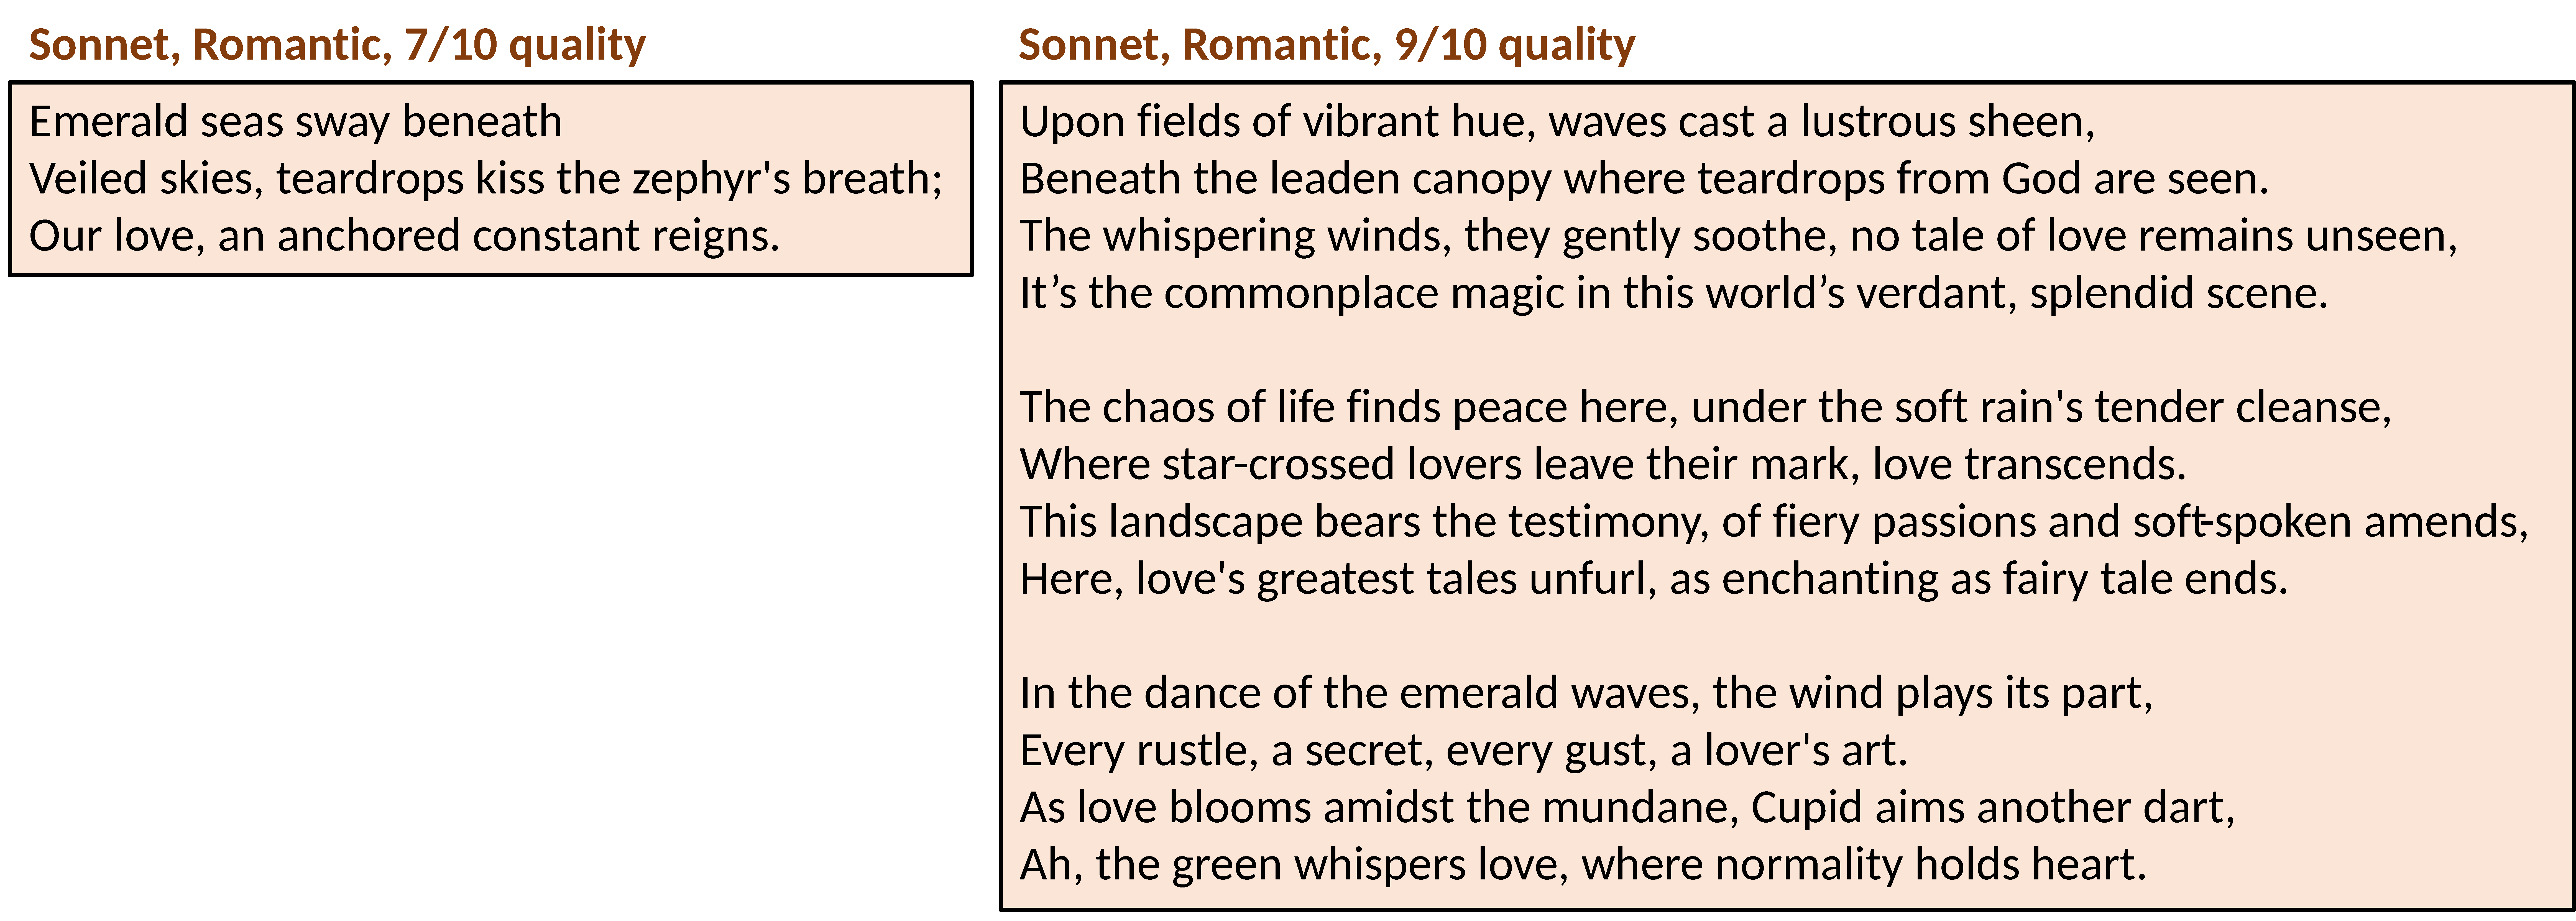
\includegraphics[width=\textwidth]{images/example_poetry2.pdf}
    \caption{Examples of different quality romantic sonnets generated and evaluated using GPT-4.}
    \label{fig:poem_examples2}
\end{figure}

\clearpage
\newpage
\subsection{On Applications of QDAIF Beyond Creative Writing}\label{app:coding_domain}
QDAIF is introduced as a viable solution for conducting creative search in subjective (e.g. creative writing) domains, from our experiments in the \textbf{Opinions}, \textbf{Stories}, and \textbf{Poetry} domains. In these domains, applying QD search to improve the quality and diversity of solutions in creative writing was not investigated in prior works due to the infeasibility of measuring such solutions with previous QD approaches, and where AI feedback (to replace expensive human feedback) is seemingly the clear best option for evaluating subjective solutions.

Yet, we also see the potential of QDAIF when applied to domains beyond creative writing, especially when coming up with solutions in such domains may require more creative brainstorming and exploration of diverse solutions that might be more intuitive through natural language assessment.

We tested QDAIF (\qdaifrewrite) in the (Python) \textbf{Code} domain, to understand how we can implement search to explore diverse solutions of interest to solve programming problems. We compared the performance of QDAIF to \textbf{Random-Code}, a simple adaptation of the \poembaseone{} which requests a solution to an instruction prompt directly, while QDAIF evolves solutions through rewriting existing code solutions. The experiment setup applies settings as described in \cref{app:poetry_setup}, except for the AI feedback prompts (cf. \cref{app:fig:code_feedback}), prompts for generating solutions (cf. \cref{app:fig:code_baseline_prompts}), and the seed solution for QDAIF (cf. \cref{app:fig:code_seed}). The aim of the \textbf{Code} domain is to generate code that is diverse in terms of "difficulty" (in readability) as well as "efficiency" of code. The "difficulty" labels are set as ["easy to read", "moderate abstraction", "highly optimized"] (with the intuition that highly optimized code is often more difficult to understand fully), while the "efficiency" labels are set as ["runtime", "balanced", "memory"] (based on the aspect of efficiency that the algorithm is more optimized for). Furthermore, we set the number of total iterations to 100, and the initialization iterations of QDAIF to 5. We based the domain problem on a task from the HumanEval benchmark \citep{chen2021codex}, specifically problem number 88, where the aim is to implement a sorting algorithm that is conditional on the properties of an unsorted list of non-negative integers. To understand the potential of each method in solving coding problems more creatively, we specified in the generation prompts to not implement solutions with the Python reserved keyword functions "sort" and "sorted", forcing the LM to come up with algorithms from scratch. The motivation for this is that we want to understand the potential of each approach in solving problems creatively, especially when viable (or subjectively preferred) solutions are not yet known in more complex domains; this constraint is one way to make the task more challenging in the \textbf{Code} domain, while encouraging a variety of approaches to sorting.

We assessed the performance of the search by both methods. QDAIF achieved a QD score of 47 (out of 90), while \textbf{Random-Code} achieved a lower QD score of 43 (out of 90). Sample efficiency with QDAIF is also higher in contrast to \textbf{Random-Code} (cf. \cref{fig:code_domain_qd_score}). All methods fill 6 out of 9 defined bins with solutions. Interestingly, none of the methods could find solutions that are "highly optimized", indicating a more general bias of the LM to generate code that is more readable, even when asked to rewrite code following a different approach. When we tested QDAIF's generated code solutions on HumanEval No. 88, 77 solutions out of 100 passed. For solutions from \textbf{Random-Code}, 78 solutions out of 100 passed. This shows that both methods are indeed generating valid, correct solutions to the task quite often, while relying purely on implementing sorting algorithms from scratch, and not implementing solutions with the default Python sorting (reserved keyword) functions.

\cref{app:table:freq_code_type_qdaif} shows the number of times QDAIF and \textbf{Random-Code} generated solutions of specific types of sorting algorithms (bubble, insertion, quick, selection, merge). In terms of the diversity assessed based on the number of times different types of sorting algorithms are implemented to solve this task, QDAIF returns noticeably more variety in the kinds of solutions it discovered to tackle the problem, with 53\% of solutions employing different sorting algorithms to the most commonly generated bubble sort approach (in contrast to \textbf{Random-Code}, where only 5\% of solutions applied non-bubble-sort approaches to the task). The variety of sorting algorithms found by QDAIF include insertion sort, quick sort, selection sort, and merge sort algorithms. \crefrange{app:fig:code_qdaif_sample_1}{app:fig:code_random_sample_2} show samples of elite code solutions from QDAIF and \textbf{Random-Code}.

The results here highlight yet again a significant open challenge in aiming for diverse, high-quality solutions from (especially RLHF) models \citep{kirk2023understanding}, as well as the improvement to diversity introduced by QDAIF approaches, and the potential of building on top of this method of search, even for domains beyond creative writing \citep{pourcel2023aces}.

\begin{figure}[ht]
    \centering
    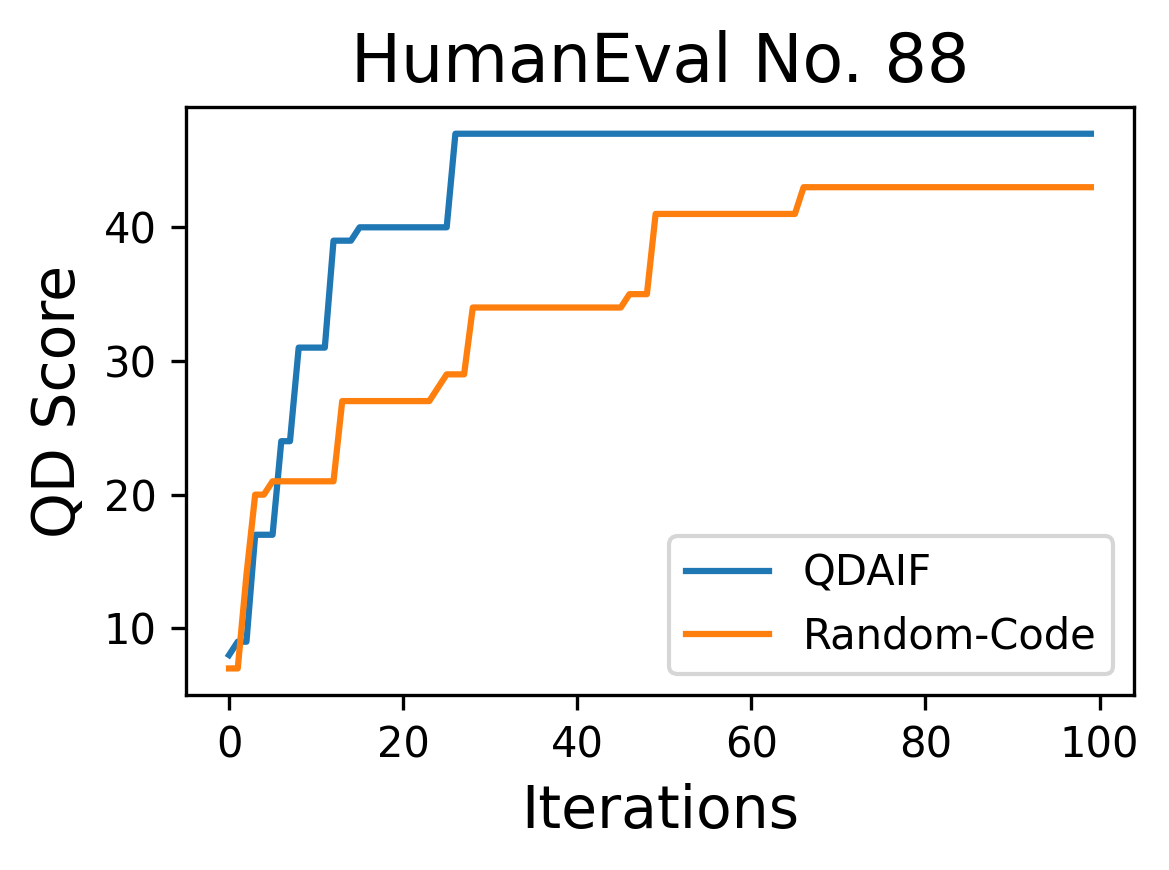
\includegraphics[width=\textwidth]{main_figures/extensions/code_domain_qd_score.png}
    \caption{\textbf{QDAIF (\qdaifrewrite) outperforms the baseline, Random-Code, in final QD score and sample efficiency.} The domain is focused on HumanEval task number 88, involving a sorting problem \citep{chen2021codex}.}
    \label{fig:code_domain_qd_score}
\end{figure}

\begin{table}[ht]
\caption{\textbf{QDAIF generates more variety in sorting algorithms implemented to solve the particular sorting task, compared to the baseline, Random-Code.} The table shows the frequency of sorting algorithms applied as the solution method across 100 generated solutions for both methods. QDAIF manages to find implementations running insertion sort, quick sort, selection sort, and merge sort, with 53\% of algorithms implemented that are not bubble sort. For the baseline, only 5\% of algorithms implemented across 100 attempt iterations (insertion and selection sort) were implemented, with 95\% of solutions based on bubble sort.}
\label{app:table:freq_code_type_qdaif}
\centering
\small
\begin{tabular}{ccccc}
\toprule
\multicolumn{5}{c}{QDAIF (\qdaifrewrite)} \\
\midrule
\textbf{Bubble} &
\textbf{Insertion} & \textbf{Quick} & \textbf{Selection} & \textbf{Merge}  \\
\midrule
47 & 20 & 19 & 12 & 2 \\
\bottomrule
\end{tabular}
\begin{tabular}{ccccc}
\toprule
\multicolumn{5}{c}{Random-Code} \\
\midrule
\textbf{Bubble} &
\textbf{Insertion} & \textbf{Quick} & \textbf{Selection} & \textbf{Merge}  \\
\midrule
95 & 1 & 0 & 4 & 0 \\
\bottomrule
\end{tabular}
\end{table}

\begin{figure}[ht]
\inputminted[mathescape,
               linenos,
               numbersep=5pt,
               gobble=0,
               frame=lines,
               framesep=2mm,
               breaklines,
               breakautoindent=true]{python}{main_figures/extensions/code_samples/qdaif_balanced_moderate_9.py}
\caption{The elite solution from QDAIF for the bin with the labels "balanced" (efficiency) and "moderate abstraction" (difficulty), as well as a quality score of 9. A quick sort approach was found here.}
\label{app:fig:code_qdaif_sample_1}
\end{figure}

\begin{figure}[ht]
\inputminted[mathescape,
               linenos,
               numbersep=5pt,
               gobble=0,
               frame=lines,
               framesep=2mm,
               breaklines, 
               breakautoindent=true]{python}{main_figures/extensions/code_samples/qdaif_runtime_easy_7.py}
\caption{The elite solution from QDAIF for the bin with the labels "runtime" (efficiency) and "easy to read" (difficulty), as well as a quality score of 7. An insertion sort approach was found here.}
\label{app:fig:code_qdaif_sample_2}
\end{figure}

\begin{figure}[ht]
\inputminted[mathescape,
               linenos,
               numbersep=5pt,
               gobble=0,
               frame=lines,
               framesep=2mm,
               breaklines, 
               breakautoindent=true]{python}{main_figures/extensions/code_samples/random_balanced_easy_8.py}
\caption{The elite solution from \textbf{Random-Code} for the bin with the labels "balanced" (efficiency) and "easy to read" (difficulty), as well as a quality score of 8. A bubble sort approach was found here.}
\label{app:fig:code_random_sample_1}
\end{figure}

\begin{figure}[ht]
\inputminted[mathescape,
               linenos,
               numbersep=5pt,
               gobble=0,
               frame=lines,
               framesep=2mm,
               breaklines, 
               breakautoindent=true]{python}{main_figures/extensions/code_samples/random_memory_moderate_7.py}
\caption{The elite solution from \textbf{Random-Code} for the bin with the labels "memory" (efficiency) and "moderate" (difficulty), as well as a quality score of 7. A bubble sort approach was found here.}
\label{app:fig:code_random_sample_2}
\end{figure}

\begin{figure}[ht]
\centering
\begin{boxedminipage}{0.98\textwidth}
\textbf{Quality Feedback Prompt:}\\
\textless{} GENERATED\_CODE \textgreater{}\\
Rate the quality of the above code snippet on a scale from 1 to 10. Answer in JSON with the key 'quality'.\\
\\
\textbf{Diversity Feedback Prompt:}\\
\textless{} GENERATED\_CODE \textgreater{}\\
Is the code runtime efficient, memory efficient, or balanced for both, choose from the following list: ["runtime", "balanced", "memory"]\\
What difficulty level is the code closest to, choose from the following list: ["easy to read", "moderate abstraction", "highly optimized"]\\

Respond in JSON with the keys "efficiency" and "difficulty".
\end{boxedminipage}
\caption{Prompts used for AI feedback evaluation with GPT-4 \citep{openai2023gpt4} on the \textbf{Code} domain. "<GENERATED\_CODE>" is where the input code is inserted as part of the prompt.}
\label{app:fig:code_feedback}
\end{figure}

\begin{figure}[ht]
\centering
\begin{boxedminipage}{0.98\textwidth}
\textbf{Random-Code:}\\
Please solve the problem below in a creative, high-quality way without using the python functions sort() and sorted(). \\
\\
Respond with only a Python function definition for `sort\_array`, and nothing else (no explanations desired either, except for code comments).\\
\\
Problem:\\
Given an array `array` of non-negative integers, return a copy of the given array after sorting, you will sort the given array in ascending order if the sum (first index value, last index value) is odd, or sort it in descending order if the sum (first index value, last index value) is even.\\
\\
Note:\\
* don't change the given array.\\
\\
Examples:\\
* sort\_array([]) =\textgreater{} []\\
* sort\_array([5]) =\textgreater{} [5]\\
* sort\_array([2, 4, 3, 0, 1, 5]) =\textgreater{} [0, 1, 2, 3, 4, 5]\\
* sort\_array([2, 4, 3, 0, 1, 5, 6]) =\textgreater{} [6, 5, 4, 3, 2, 1, 0]\\
\\
\textbf{\qdaifrewrite{} (QDAIF):}\\
\textless{} PARENT\_CODE \textgreater{}\\
Please rewrite the code above into a new solution with a different creative, high-quality approach, without using the python functions sort() and sorted().\\
\\
Respond with only a Python function definition for `sort\_array`, and nothing else (no explanations desired either, except for code comments).\\
\\
Problem:\\
Given an array `array` of non-negative integers, return a copy of the given array after sorting, you will sort the given array in ascending order if the sum (first index value, last index value) is odd, or sort it in descending order if the sum (first index value, last index value) is even.\\
\\
Note:\\
* don't change the given array.\\
\\
Examples:\\
* sort\_array([]) =\textgreater{} []\\
* sort\_array([5]) =\textgreater{} [5]\\
* sort\_array([2, 4, 3, 0, 1, 5]) =\textgreater{} [0, 1, 2, 3, 4, 5]\\
* sort\_array([2, 4, 3, 0, 1, 5, 6]) =\textgreater{} [6, 5, 4, 3, 2, 1, 0]\\
\end{boxedminipage}
\caption{Prompts used by each method for generating code with GPT-4 \citep{openai2023gpt4}.}
\label{app:fig:code_baseline_prompts}
\end{figure}

\begin{figure}[ht]
\inputminted[mathescape,
               linenos,
               numbersep=5pt,
               gobble=0,
               frame=lines,
               framesep=2mm]{python}{main_figures/extensions/seed_code.py}
\caption{Seed program for the coding domain, to initialize QDAIF search. This is from a model completion that was obtained through standard prompting of the LM (the \textbf{Random-Code} baseline approach of requesting solutions directly).}
\label{app:fig:code_seed}
\end{figure}
